\documentclass[a4paper, twoside, table, 10pt]{report}

%% Language and font encodings
\usepackage[english]{babel}
\usepackage[utf8x]{inputenc}
\usepackage[T1]{fontenc}
\usepackage{tikz}
\usepackage{xcolor}
\usepackage{pbox}

\usetikzlibrary{er,positioning}
\usetikzlibrary{shapes.misc}

%% Sets page size and margins
\usepackage[a4paper,top=3cm,bottom=2cm,left=3cm,right=3cm,marginparwidth=1.75cm]{geometry}

%% Useful packages
\usepackage{amsmath}
\usepackage{amssymb}
\usepackage{amsthm}
\usepackage{enumitem}
\usepackage{mathpartir}
\usepackage{csquotes}
\usepackage{cite}
\usepackage{titlesec}
\usepackage{graphicx}
\usepackage[colorinlistoftodos]{todonotes}
\usepackage[colorlinks=true, allcolors=blue]{hyperref}
\usepackage{float}
\floatstyle{boxed} 
\restylefloat{figure}
\usepackage{mathtools}
\usepackage{caption}
\usepackage{subcaption}
\usepackage{listings}
\usepackage{multirow}
\usepackage{wasysym}

\usepackage{xcolor}


\definecolor{codegreen}{rgb}{0,0.3,0}
\definecolor{codegray}{rgb}{0.5,0.5,0.5}
\definecolor{codepurple}{rgb}{0.58,0,0.82}
\definecolor{backcolour}{rgb}{1,1,1}

\lstdefinestyle{mystyle}{
    backgroundcolor=\color{backcolour},   
    commentstyle=\color{codegreen},
    keywordstyle=\color{codegreen},
    numberstyle=\tiny\color{codegray},
    stringstyle=\color{codepurple},
    basicstyle=\ttfamily\footnotesize,
    breakatwhitespace=false,         
    breaklines=true,                 
    captionpos=b,                    
    keepspaces=true,                 
    numbers=left,                    
    numbersep=5pt,                  
    showspaces=false,                
    showstringspaces=false,
    showtabs=false,                  
    tabsize=2,
    escapeinside={(*@}{@*)}
}
 
\lstset{style=mystyle}

\newcommand{\highlight}[1]{%
  \colorbox{gray!40}{$\displaystyle#1$}}
  
\newcommand{\highcode}[1]{%
  \highlight{\texttt{#1}}}

\newcommand{\extract}{\mathrlap{-}\triangleright}
\newtheorem{lemma}{Lemma}

\newcommand{\rulesep}{\unskip\ \vrule\ }


\titleformat{\chapter}[block]
  {\normalfont\huge\bfseries}{\thechapter.}{1em}{\Huge}
\titlespacing*{\chapter}{0pt}{-19pt}{10pt}

\title{Type Constraints and Deny Capabilities}
\author{Michael Gillan}
% Update supervisor and other title stuff in title/title.tex

\begin{document}
\begin{titlepage}

\newcommand{\HRule}{\rule{\linewidth}{0.5mm}} % Defines a new command for the horizontal lines, change thickness here

%----------------------------------------------------------------------------------------
%	LOGO SECTION
%----------------------------------------------------------------------------------------


\includegraphics[width=8cm]{title/logo.png}\\[1cm] % Include a department/university logo - this will require the graphicx package
 
%----------------------------------------------------------------------------------------

\center % Center everything on the page

%----------------------------------------------------------------------------------------
%	HEADING SECTIONS
%----------------------------------------------------------------------------------------

\textsc{\LARGE MEng Individual Project}\\[1.5cm] % Name of your university/college
\textsc{\Large Imperial College London}\\[0.5cm] % Major heading such as course name
\textsc{\large Department of Computing}\\[0.5cm] % Minor heading such as course title

%----------------------------------------------------------------------------------------
%	TITLE SECTION
%----------------------------------------------------------------------------------------
\makeatletter
\HRule \\[0.4cm]
{ \huge \bfseries \@title}\\[0.4cm] % Title of your document
\HRule \\[1.5cm]
 
%----------------------------------------------------------------------------------------
%	AUTHOR SECTION
%----------------------------------------------------------------------------------------

\begin{minipage}{0.4\textwidth}
\begin{flushleft} \large
\emph{Author:}\\
\@author % Your name
\end{flushleft}
\end{minipage}
~
\begin{minipage}{0.4\textwidth}
\begin{flushright} \large
\emph{Supervisor:} \\
Prof. Sophia Drossopoulou \\[1.2em] % Supervisor's Name
\emph{Second Marker:} \\
Prof. Nobuko Yoshida % second marker's name
\end{flushright}
\end{minipage}\\[2cm]
\makeatother

% If you don't want a supervisor, uncomment the two lines below and remove the section above
%\Large \emph{Author:}\\
%John \textsc{Smith}\\[3cm] % Your name

%----------------------------------------------------------------------------------------
%	DATE SECTION
%----------------------------------------------------------------------------------------

{\large \today}\\[2cm] % Date, change the \today to a set date if you want to be precise

\vfill % Fill the rest of the page with whitespace

\end{titlepage}

\begin{abstract}
%Your abstract goes here

Generics are a vital and powerful part of nearly all modern programming languages, which allow code reuse across various types. However, with great power comes great responsibility; generics, and how they interact with the rest of a language, are highly complex, and in some cases require immense programmer effort to understand and apply. \\

Generic variables are usually bounded using subtyping; the range of types a variable is permitted to be is defined by the subtype of its bound. When types are referred to in their bounds, known as f-bounded polymorphism, the situation gets more complicated still. \\

An alternative to subtype bounding has been proposed in Genus, a type system developed on top of Java that uses type predicates known as constraints to bound type variables. Genus is highly expressive and powerful, but lacks a proof of soundness. \\

We present Genus-, a distilled, imperative formal model of generics that uses the same generic mechanisms as Genus. We discuss the well-formedness of the system, and show that it is sound. \\

We also describe DeGen, a type system we designed to incorporate the deny capabilities and actor-based execution from Pony into Genus-. We define its well-formedness, and discuss proving preservation of soundness and data-race freedom.

\end{abstract}

\renewcommand{\abstractname}{Acknowledgements}
\begin{abstract}

I would like to thank my supervisor, Sophia Drossopoulou, for her incredible patience and guidance over the course of this project. Her feedback and support has been vital for getting this project off the ground. \\

I'd also like to thank my family, for not getting mad when I didn't return their calls, and my flatmates for putting up with the replica North Atlantic garbage patch slowly migrating out of my room. \\

And finally, a shout-out to Michel Jouvet, without whose works on analeptics, this project would not and could not possibly exist. RIP to a real one.

\end{abstract}

\tableofcontents
%\listoffigures
%\listoftables

\chapter{Introduction}

\section{Motivations}

There is inherent complexity in writing concurrent applications; care must be taken to prevent concurrent operations from interfering with each others' data as it could potentially create data races. The widely used solution this problem is explicit concurrency management through concurrency primitives. These require programmers to be able to reason about how threads will interact with each other, and to be constantly mitigating against concurrency issues. Despite this additional burden on programmers, they are exposed to risks such as deadlocking. \\

A solution to relieve the burden of concurrency on programmers is actor-based languages with capability systems; augmented type systems that can statically check that programs are data-race free. One such language is Pony, which uses a system called \textit{deny capabilities} to determines what can and cannot be done with every reference in a program. \\

Like many other object-oriented programming languages, Pony uses a system of generics based on bounding type variables by subtyping. This is powerful and expressive, but can lead to unsoundness and programmer burden, especially when types appear in their own type bounds. This is referred to as `f-bounded polymorphism`. Recently, alternative systems of generics have been developed, which constrain generic type variables using mechanics other than subtyping. \\

One alternative to f-bounded polymorphism is to use type predicates to ensure the interfaces that types present to generic code have an expected structure, without creating a subtype relation between the type and the interface definition. This is the approach taken by Genus\cite{Zhang2015}, a highly expressive system of generics built on top of Java that uses type predicates (called \textit{constraints}) to bound type variables. \\

We give a minimal formal specification of the ideas presented in Genus, and prove that it is sound. On top of this model, we introduce deny capabilities, resulting in a minimal, sound proof of concept that marries the major ideas from both systems.

\section{Contributions}

This project presents Genus-, a formal specification for the mechanism of genericity presented in Genus. We describe an augmented type system incorporating deny capabilities, DeGen, so as to provide an alternative to generics as they currently exist in Pony.

\begin{itemize}
    \item We developed Genus-, a distilled, minimal formal model for the mechanism of genericity presented in Genus. This is an imperative model, which is more faithful to real programming languages and allows us to uncover more possibilities for unsoundness. It is described in Chapter \ref{chpt:genus-}
    
    \item We give a proof of soundness for Genus- in Section \ref{sec:genus-sound}. Genus does not have a proof of soundness, so this is a novel contribution that establishes Genus- as a valid basis for designing a more complex type system on top of.
    
    \item We designed DeGen, an augmented version of Genus- that includes deny capabilities. We describe the design process in \ref{chpt:degen} 
    
    \item We also give a formal description of DeGen in Chapter \ref{chpt:degen}, and discuss some thoughts about how we would show soundness and preservation of well-formed visibility. Our formal description includes a parametric formulation of viewpoints, based on previously established requirements.
\end{itemize}
\chapter{Background}

\section{Types and Type Systems}

Type systems are lightweight formal methods that allow a programmer to reason that a program will behave as intended with respect to a specification of the language it is created in. In his book \textit{Types and Programming Languages}\cite{PierceBenjaminC2002Tapl}, Pierce defines a type system:
\begin{displayquote}
A type system is a tractable syntactic method for proving the absence of certain program behaviours by classifying phrases according to the kinds of values they compute.
\end{displayquote}
From this definition, we can infer that types are the "kinds of values" that can result from computations within a program.

Traditionally, the concept of a \textit{record type} is used to define composite types made from more than one primitive type; a record, which can be thought of as an \textit{object} with its components representing the object's methods and fields, is an unordered set of labeled values, and a record type is specified by associating a type with each of its labels \cite{Cardelli1985}. In addition to composite and primitive types, we also have function types, which express the types of the parameters and the return type of a function.

Formally, a record consists of labels $x_1, ..., x_j$ with associated types $\sigma_1, ... \sigma_j$, and is represented as the set $\{x_1:\sigma_1, ..., x_j:\sigma_j\}$ \cite{Canning1989}.

\subsection{Structural Type Systems}

A structural type system is one in which type equivalence and compatibility is determined entirely by the type's structure; two types are compatible if for each feature in the first type, a corresponding and equivalent feature exists in the second type.

A language that employees this sort of type system is Go, when checking against interfaces. In the example below, \texttt{fmt.Println()} expects the parameter to implement the \texttt{fmt.Stringer} interface, which requires a method \texttt{String() string}. Since \texttt{User} implements this, it is accepted by \texttt{fmt.Println()}

\begin{verbatim}
  type User struct {
    name string
  }

  func (user User) String() string {
    return fmt.Sprintf("User: name = %s", user.name)
  }

  func main() {
    user := User{name: "foo"}
    fmt.Println(user)         // User: name = foo
  }
\end{verbatim}

\subsection{Nominal Type Systems}

A nominal type system is one in which type equivalence and compatibility is determined entirely by type declarations and names; two structurally identical types are not considered the same if they are declared with different names.

The Java example given below shows that, although \texttt{Customer} and \texttt{Employee} are structurally identical, they cannot be assigned to each other.

\begin{verbatim}
  class Customer {
    String name;
  }

  class Employee {
    String name;
  }

  class Main {
    public static void main(String[] args) {
      Customer c = new Customer(); 
      Employee e = new Employee();
      c = e; // incompatible types
    }
  }
\end{verbatim}

\subsection{Union and Intersection Types}

Union and intersection types are forms of type expressions that allow the combination of types into more complex types, without the need for a definition.

\subsubsection{Union Types}

A union type describes values that belong to either of two types. A good example of this is \texttt{char} in C. A signed char generally has a range of -127 to 128, and an unsigned char has a range of 0 to 255. The union of a signed char and unsigned char could accept values in the range -127 to 255. Generally, valid operations on union types have to be valid of both of its component types.

\subsubsection{Intersection Types}

An intersection type describes values that belong to both of two types. Using the char example above, the intersection type of a signed and unsigned char would accept values in the range 0 to 128. This intersection type could then be used in any operation expecting either of its component types, because it is compatible with both.

\section{Subtyping}

A type S is a structural subtype of T if S’s interface (its public fields and methods) is a superset of T’s. Intuitively, any operation that we perform on T through its interface can also be performed on S.
Formally, we can use the concept of a record type, which describes the interface of an object as a mapping of labels to types. The record subtyping axiom is a formalization of the intuition above:

\begin{mathpar}
\inferrule{\sigma_1 \subseteq \rho_1, ..., \sigma_k \subseteq \rho_k}{\{x_1:\sigma_1, ...,  x_k:\sigma_k, ..., x_l:\sigma_l\} \subseteq \{x_1:\rho_1, ...,  x_k:\rho_k\} }
\end{mathpar}

Nominal subtyping is an explicitly defined subtype relation between two types. The below example shows nominal subtyping in Java; the relationship between ‘Bob’ and ‘Named’ is declared, and says that ‘Bob’ implements ‘Named’.
\begin{verbatim}
interface Named {
    public String name();
}

class Bob implements Named {
    public String name() {
        return "Bob";
    }
}
\end{verbatim}
With nominal subtyping, it is the compiler’s responsibility to check that the subtype implements everything required by the subtyping relation.

\section{Covariance and Contravariance}

The concept of variance refers to how the subtyping between complex type expressions relates to the subtyping of the components of said expressions; the type constructor of complex types may preserve, reverse, or ignore the subtype relation between its component types.

A covariant type constructor is one that preserves the relationship between subtypes; if \texttt{foo} is a subtype of \texttt{bar}, and the type constructor of a \texttt{List} is covariant, then a \texttt{List<foo>} is a subtype of \texttt{List<bar>}.

A contravariant type constructor is one that reverses the relationship between subtypes; given the same subtype relationship between \texttt{foo} and \texttt{bar}, and a contravariant type constructor for a \texttt{Printer}, we have that \texttt{Printer<bar>} is a subtype of \texttt{Printer<foo>}.

Additionally, there is the concept of invariance, where the relationship between simple types is ignored in complex type constructors, and two different instances of a type constructor are neither a subtype or a supertype of one another.

When typing a function, the return type may be covariant when the function is overridden, and parameter types may be contravariant. Generally, wherever the base method's function may be called, the overridden function must be permitted.
Consider the psuedocode example below.

\begin{verbatim}
  class Foo extends Bar {}
  class Foo1 extends Bar1 {}

  class Thing {
    Bar doThing(Foo1 x) { 
      // implementation
    }
  }

  class OtherThing extends Thing {
    Foo doThing(Bar1 x) {
      // implementation
    }
  }
\end{verbatim}
First, it is clear that \texttt{OtherThing} can make \texttt{doThing} return a \texttt{Foo} as \texttt{Foo} is a subtype of \texttt{Bar}, and intuitively anything expecting a \texttt{Bar} can use a \texttt{Foo} instead. Secondly, \texttt{otherThing} can make \texttt{doThing} take a \texttt{Bar1} as a parameter since anything calling \texttt{Thing.doThing} must pass a \texttt{Foo1}, which is guaranteed to be a subtype of \texttt{Bar1}, and can be treated that as a \texttt{Bar1.}

The above leads to a standard rule for function subtyping (using the arrow for function typing):

\begin{mathpar}
\inferrule{\sigma' \subseteq \sigma \\ \tau \subseteq \tau'}{\sigma \to \tau \subseteq \sigma' \to \tau'}
\end{mathpar}

Some languages, such as Java, limit parameter types to be invariant, while others including C\# allow parameter types to be contravariant.

\section{Polymorphism} \label{polymorphism}

Polymorphism is defined as providing a single interface to entities of different types \cite{Stroustrup}. 

\subsection{Ad hoc Polymorphism}

Ad hoc polymorphism, commonly referred to as \textit{function overloading}, is the mechanism by which a function appears to work on multiple different types, even if these types do not share a similar structure \cite{Cardelli1985}. 

The common example for this is the \texttt{+} operator; when applied to integers, we have operations of the form \texttt{1 + 2 == 3}, where \texttt{+} is a summation function; when applied to strings, we can use it to perform concatenation, such as \texttt{"foo" + "bar" == "foobar"}. It is therefore clear that although this operator presents the same interface for many different types, it actually represents a number of distinct, heterogeneous functions.

\subsection{Subtype Polymorphism}

Since we know that subtypes present the same interface as their base type, polymorphism through subtyping allows a subtype to be used anywhere a supertype is expected. This is clear in the below example:
\begin{verbatim}
  class A {}
  class B {}

  class Pair {
    Object fst;
    Object snd;
    
    Pair(Object fst, Object snd) {
        this.fst = fst;
        this.snd = snd;
    }
    
    Object getFst() {
        return this.fst;
    }
  }

  class Main {
    public static void main(String[ ] args) {
      Pair pairA = new Pair(new A(), new A());
      Pair pairB = new Pair(new B(), new B());
    }
  }
\end{verbatim}
Both \texttt{A} and \texttt{B} can be stored using the same \texttt{Pair} class, as they are both subtypes of \texttt{Object}. However, all type information is lost once the reference is stored. The following execution produces an error, as \texttt{getFst()} will only return an \texttt{Object}.
\begin{verbatim}
  class Main {
    public static void main(String[] args) {
      Pair pairA = new Pair(new A(), new A());
        
      A a = pairA.getFst(); // incompatible types
    }
  }
\end{verbatim}

\subsection{Parametric Polymorphism}

Parametric polymorphism allows a single implementation of a function to work uniformly on many different types, which usually have some common structure. They are said to be \textit{generic} and accept type parameters as placeholders for types:

\begin{verbatim}
  class Pair<T> {
    T fst;
    T snd;
    
    Pair(T fst, T snd) {
        this.fst = fst;
        this.snd = snd;
    }
    
    T getFst() {
        return this.fst;
    }
  }

  class Main {
    public static void main(String[] args) {
      Pair<A> pairA = new Pair(new A(), new A());
        
      A a = pairA.getFst(); // successful
    }
  }
\end{verbatim}
The above leads to a successful execution, as the type information about \texttt{fst} is preserved through the type parameter. The parameter \texttt{T} is unbounded, and ranges over all possible types.

Bounded quantification allows us to specify type parameters that range over a subset of all types. Generally, this set is given by all subtypes of a given type.

\begin{verbatim}
  interface Stringable {
    public String string();
  }

  class A implements Stringable {
    public String string() {
      return "A";
    }
  }

  class Pair<T extends Stringable> implements Stringable {
    T fst;
    T snd;
    
    Pair(T fst, T snd) {
      this.fst = fst;
      this.snd = snd;
    }
    
    public String string() {
      return this.fst.string() + ", " + this.snd.string();
    }
  }

  class Main {
    public static void main(String[] args) {
      Pair<A> pairA = new Pair(new A(), new A());
         
      System.out.println(pairA.string()); // "A, A"
    }
  }
\end{verbatim}
Here \texttt{T} can be any subtype of \texttt{Stringable}.

\subsection{F-bounded Polymorphism}

Recursively bounded quantification, also known as f-bounded quantification, allows type parameters to appear in their own bounds.
\begin{verbatim}
  interface Equatable<T extends Equatable<T>> {
    public boolean eq(T that);
  }
\end{verbatim}
In the above, the type parameter \texttt{T} is required to be a subtype of \texttt{Equatable[T]}. This means, if \texttt{String} were to implement \texttt{Equatable[String]}, it would require a method \texttt{boolean eq(String that)}. This means that \texttt{Strings} are comparable to other \texttt{Strings} but not to, say, \texttt{Integers}.

\subsection{Issues with F-Bounded Polymorphism}

F-bounded polymorphism introduces type-checking complexities. It requires that inheritance to be recursive; \texttt{String} implements \texttt{Comparable<String>}, meaning it is defined in terms of its inherited type. When recursive inheritance is mixed with variance in type parameters, polymorphic subtyping becomes undecidable \cite{Kennedy2008}. However, this does not apply in Pony, due to type invariance relative to type parameters. 

F-bounded polymorphism can lead to significant code complexity. Below is an example of two classes taken from the \textit{FindBugs} \cite{FindBugs} open-source project.
\begin{verbatim}
    class AbstractVertex<
        EdgeType extends AbstractEdge<EdgeType, ActualVertexType>, 
        ActualVertexType extends AbstractVertex<EdgeType, ActualVertexType>> {...}
    class AbstractEdge <
        ActualEdgeType extends AbstractEdge<ActualEdgeType, VertexType>, 
        VertexType extends AbstractVertex<ActualEdgeType, VertexType>> {...}
\end{verbatim}
The mutual dependency between \texttt{AbstractVertex} and \texttt{AbstractEdge} leads both classes to have very complex signatures.

\section{Genus, Models and Constraints} \label{sec:genus-bg}

An alternative generics mechanism to subtyping is presented in Genus \cite{Zhang2015}, a system where named constructs, called models, explicitly witness constraints. 

\subsection{Constraints}

In Genus, types are constrained using explicit \textit{type constraints} that exist as a predicate on types. To require that a type has, for example, an \texttt{equals(...)} method, the below constraint can be used:

\begin{verbatim}
  constraint Eq[T] {
    boolean equals(T that);
}
\end{verbatim}

This constraint can then be applied to type parameters to establish the ability to test equality on them:

\begin{verbatim}
  interface Set[T where Eq[T]] { ... }
\end{verbatim}

Thus, an instantiation of \texttt{Set} requires a model, supplied either implicitly by the compiler or chosen explicitly by the programmer, to witness that \texttt{Eq[T]} is satisfied by whatever the type argument \texttt{T} is.

\subsubsection{Prerequisite Constraints}

Constraints may have other constraints as their prerequisites, and the satisfaction of a constraint entails the satisfaction of its prerequisite constraints. For example, \texttt{Eq[T]} is prerequisite of \texttt{Comparable[T]}, and the relationship can be expressed as:

\begin{verbatim}
  constraint Comparable[T] extends Eq[T] {
    int compareTo(T other);
  }
\end{verbatim}

\subsection{Models}

Models are witnesses of constraints that are provided with the type argument.

\subsubsection{Natural Models}

If a type structurally conforms to a constraint, i.e. already has the required operations, then it forms a natural model for the constraint. For example, \texttt{String} has a built-in \texttt{equals(...)} method, and so \texttt{Set[String]} can use this method for establishing equality.

\subsubsection{Explicit Models}

The programmer can create models to satisfy a constraint if a natural model does not exist or does not have the desired behaviour. For example, case-insensitive equality can be defined as a model for \texttt{Eq[String]}:

\begin{verbatim}
  model CIEq for Eq[String] {
    bool equals(String str) {
      return equalsIgnoreCase(str);
    }
  }
\end{verbatim}

Models can be extended and reused through model inheritance; a model for \texttt{Comparable[String]} can reuse the \texttt{CIEq} model for \texttt{Eq[String]}:

\begin{verbatim}
  model CICmp for Comparable[String] extends CIEq {
    int compareTo(String str) {
      return compareToIgnoreCase(str);
    }
  }
\end{verbatim}
Alternatively, \texttt{CICmp} could define its own \texttt{equals(...)} method.
    
The model chosen to witness a constraint on a type is contained as part of the type; this is illustrated below:

\begin{verbatim}
  Set[String] s0;
  Set[String with CIEq] s1;
  s1 = s0; // illegal assignment: different types.
\end{verbatim}

The model of equality chosen for each \texttt{Set} is a static part of the type, and so \texttt{s0} and \texttt{s1} represent different types.

\section{Dependent Types}

A dependent type is one defined based upon a value. For example, a "pair of integers" is a type, and a "pair of integers where the first value is greater than the second" is a dependent type. Pony does not have dependent types, but an example, adapted from \cite{Bove2009}, in Agda, a language that does, is below: 
\begin{verbatim}
    Vec : Set -> Nat -> Set
    Vec A zero = Unit
    Vec A (succ n) = A X Vec A n
\end{verbatim}
The signature of a \texttt{zip} function, which requires both \texttt{Vec} to be of the same length, can be defined as:
\begin{verbatim}
    zip : {A B : Set} -> (n : Nat) ->
        Vec A n -> Vec B n -> Vec (A X B) n
\end{verbatim}

We can draw a parallel with polymorphic types: polymorphic types are parameterised by types, and dependent type are parameterised by values.

\subsection{Path Dependent Types}

Path dependent types are a form of dependent type which depends on the value of an abstract type parameter.
In Scala, a nested type depends on a specific instance of the outer type, rather than the outer type itself.
\begin{verbatim}
  trait Animal { a =>
    type Food
    def eats(food: a.Food): Unit = {}
  }

  trait Grass
  trait Meat

  trait Cow extends Animal with Meat {
    type Food = Grass
  }

  trait Lion extends Animal {
    type Food = Meat
  }
\end{verbatim}
In the definitions above, adapted from \cite{Amin2014}, \texttt{Animal} has an \textit{abstract type member} \texttt{Food}. We can see that \texttt{eats} requires its parameter to be of type \texttt{a.Food}, which is a \textit{path-dependent type}. We therefore define \texttt{Cow} to be an \texttt{Animal} that eats \texttt{Grass}, and \texttt{Lion} to be an \texttt{Animal} that eats \texttt{Meat}.
\begin{verbatim}
  val leo = new Lion {}
  val milka = new Cow {}
  val daisy = new Cow {}

  leo.eats(milka)     //ok
  milka.eats(daisy)   //error
\end{verbatim}
Whilst \texttt{leo} can eat \texttt{milka}, since \texttt{leo.eats()} expects type \texttt{Meat} which \texttt{milka} is, \texttt{milka} cannot eat \texttt{daisy} as she isn't \texttt{Grass}.

\section{Soundness}

A sound type system is one in which well-typed programs cannot lead to type errors \cite{Wright1994}. We can prove the type soundness of a system using \textit{subject reduction} and \textit{progress} \cite{Igarashi2001}.

\subsubsection{Subject Reduction}

A type system with subject reduction says that the evaluation of expressions does not cause their type to change. This can be expressed formally with the type rule:

\begin{mathpar}
\inferrule{\Gamma \vdash e_1 : \tau \\ e_1 \to e_2}{\Gamma \vdash e_2 : \tau}
\end{mathpar}

\subsubsection{Progress}

Progress indicates that the evaluation of a program cannot become \textit{stuck}. This means that each program can either be evaluated infinitely, or will reach a state in which it cannot be evaluated further, that is, a value or a type error; the program never gets into an undefined state where no further transitions are possible.

\subsubsection{Type Soundness}

By combining the above mechanisms, if we can show that a well-typed program \footnote{We consider the entire program to be an expression for the definitions above.} reduces to only other well-typed programs, and will never become stuck, we have shown that the system is type sound.

\subsection{Proving Type Soundness in the Presence of Generics}

To prove that a generic type system is sound given a proof of soundness for a non-generic version for the same system, it is sufficient to show that any valid type instantiation on a generic declaration yields a valid concrete declaration \cite{Gordon2012} .

% \section{Concurrent Programs} \label{conrules}

\section{Actor Based Models}

Actor based languages \cite{Hewitt1973} provide a simpler model of concurrency than traditional object-oriented languages; instead of relying on mutual exclusion primitives to control threads' access to shared memory, \textit{actors} have their own private state which only they can modify, and rely on message passing to interact with other actors. Actors process messages sequentially, but can execute concurrently. This message passing system eliminates the need for concurrency primitives such as locks and semaphores, and grants data race freedom.

\subsection{Capabilities}

In languages where the programmer can use pointers to reference objects in the heap, a number of potential problems can occur; the aliasing and sharing of mutable state can lead to unintended behaviour.

A solution to this problem is \textit{capabilities}. In the system proposed by \cite{Boyland2001}, capabilities consist of a pointer to an object, and a set of access rights that detail how the pointer can be used. \cite{Boyland2001} introduces the concepts of \textit{base rights} and \textit{exclusive rights}; base rights say a reference can perform an operation, such as writing, on an object, and exclusive rights say that no other reference can perform that operation on the object\footnote{This does not necessarily mean the reference can perform the operation, it would still require the base right to do so.}. This leads to the concept of \textit{compatibility} -- two capabilities on the same object are compatible if their access rights permit the other to exist. Corresponding base and exclusive rights are incompatible as asserting one denies other references of the other.

\subsubsection{Capabilities in Actor Based Models}

We can use capabilities in actor based models to ensure data-race free programs. By ensuring that all references to an object have compatible capabilities, which can be ensured by the type system statically, we know that no two actors can access the same memory in a way that causes a data-race.

Capabilities in actor models give actors the ability to read, mutate, and send a reference safely. Only one actor may possess a mutable reference to an object at a time, and so to send a mutable reference, the sending actor must give up its reference to the object \cite{Srinivasana}.



\subsubsection{Isolation} \label{isolation}

An isolated reference is one where all paths to non-immutable objects reachable from the reference pass through it \cite{Gordon2012}. These isolated references form static regions where mutable objects reachable from the reference can only be reached through the reference, and immutable objects must be either only reachable through the reference of globally immutable \cite{Clebsch2015}.

We can \textit{recover} mutable types back to an isolated state if we can ensure it is an isolated reference. The resulting alias makes stronger local guarantees than the previous mutable alias.

\subsection{Deny Capabilities}

While earlier capability systems \cite{Srinivasana, Gordon2012, Boyland2001} detail what operations are allowed on an object, an other approach is to use capabilities to detail what aliases are \textit{denied} by the existence of a reference \cite{Clebsch2015}. This system of deny capabilities is what we will use to frame the rest of our exploration.

\subsubsection{Aliases}

\textbf{Local aliases} are other references in the same actor to an object that the actor already has a reference to. \textbf{Global aliases} are references to the object that are held by other actors. Deny capabilities describe what a local and global alias is forbidden to do.

A reference is mutable if it denies global read and write aliases, as no other actor can concurrently read or write to the object. Immutability is given by denying global write aliases, so a data race where an actor is reading an object as another is writing to it cannot occur. Denying no glabal aliases makes a reference \textit{opaque}, meaning it can be neither read nor written to.

A reference can be safely sent to another actor if its global and local deny properties are the same, i.e. it does not matter which actor is holding the reference.

A full description of the deny capabilities is given in Table \ref{table:cap}.

\begin{table}[h]
\centering
\begin{tabular}{l|l|l|l|l}
\cline{2-4}
                                                                                               & \begin{tabular}[c]{@{}l@{}}Deny global read/ \\ write aliases\end{tabular} & \begin{tabular}[c]{@{}l@{}}Deny global \\ write aliases\end{tabular} & \begin{tabular}[c]{@{}l@{}}Allow all \\ global aliases\end{tabular} &  \\ \cline{1-4}
\multicolumn{1}{|l|}{\begin{tabular}[c]{@{}l@{}}Deny local read/\\ write aliases\end{tabular}} & \textit{Isolated (iso)}                                                   &                                                                      &                                                                     &  \\ \cline{1-4}
\multicolumn{1}{|l|}{\begin{tabular}[c]{@{}l@{}}Deny local \\ write aliases\end{tabular}}      & Transition (\texttt{trn})                                                          & \cellcolor[HTML]{C0C0C0}\textit{Value (val)}                         &                                                                     &  \\ \cline{1-4}
\multicolumn{1}{|l|}{\begin{tabular}[c]{@{}l@{}}Allow all \\ local aliases\end{tabular}}       & Reference (\texttt{ref})                                                           & \cellcolor[HTML]{C0C0C0}Box (\texttt{box})                                    & \cellcolor[HTML]{656565}\textit{Tag (tag)}                          &  \\ \cline{1-4}
                                                                                               & (Mutable)                                                                 & \cellcolor[HTML]{C0C0C0}(Immutable)                                  & \cellcolor[HTML]{656565}(Opaque)                                    &  \\ \cline{2-4}
\end{tabular}
\caption{Capability matrix, reproduced from \cite{Clebsch2015}}
\label{table:cap}
\end{table}

\subsection{View Point Adaptation}

\begin{figure}[h]
    \centering
    
\begin{tikzpicture}[auto,node distance=1.5cm]
  \node[entity] (node1) {$\alpha$};
  \node[entity] (node2) [below = of node1] {$\iota_1$};
  \node[entity] (node3) [below = of node2]	{$\iota_2$};
  \draw[->] (node1)
    edge	 node {$x, \kappa$}    (node2);
  \draw[->] (node2)
    edge	 node {$f, \kappa'$}	(node3);
  \draw[dashed,->] (node1)
    edge[bend left=90]   node {$x.f, \kappa \triangleright \kappa'$} (node3);  
\end{tikzpicture}

    \caption{Viewpoint Adaptation}
    \label{fig:viewpoint}
\end{figure}

When reading a field from an object, as seen in Figure \ref{fig:viewpoint}, we create a temporary alias whose capability depends on the capabilities of the object and its field. We call this \textit{viewpoint adaptation}, denoted by $\triangleright$ and it can intuitively be thought of as "if \textit{$a_1$} sees \textit{$a_2$} as $\kappa$ and \textit{$a_2$} sees \textit{$a_3$} as $\kappa'$, then \textit{$a_1$} sees \textit{$a_3$} as  $\kappa \triangleright \kappa'$ \cite{Cunningham2008}. This alias is \textit{temporary}, and does not outlive the execution of the expression which created it, such as field read \cite{Clebsch2015}.

\subsection{Extracting Adaptation} \label{extracting}

\begin{figure}[h]
    \centering
    \begin{tikzpicture}[auto,node distance=1.5cm]
  \node[entity] (node1) {$\alpha$};
  \node[entity] (node2) [below = of node1] {$\iota_1$};
  \node[entity] (node3) [below = of node2]	{$\iota_2$};
  \draw[->] (node1)
    edge	 node {$x, \kappa$}    (node2);
  \draw[->] (node2)
    edge	 node{$f, \kappa'$}    (node3);
  \draw[dashed,->] (node1)
    edge[bend left=90]   node {$x.f, \kappa \extract \kappa'$} (node3);  
\end{tikzpicture}
    \caption{Extracting Adaptation}
    \label{fig:extracting}
\end{figure}

The extracting adaptation introduced by Steed \cite{Steed2016} considers the case in Figure \ref{fig:extracting}, where an actor $\alpha$ has an object $x$, which in turn has a field $f$. If $f$ is overwritten with a new value, the return value of the operation is a temporary reference to the old value of the field, whose reference capability is given by $\kappa \extract \kappa'$.

\subsection{Aliasing and Unaliasing}

\subsubsection{Temporary References} \label{sec:bg-temp}

Here, we distinguish between stable references, such as object fields and local variables, and temporary references, such as those created by the adaptations described above.

Considering the capabilities of temporary aliases, we are presented with two additional scenarios which affect unique aliases:

\begin{itemize}
    \item zero stable references exist to an object anywhere in the program. This is similar to the isolation described in Section \ref{isolation}, but its sole reference is temporary (it has one reference removed). This is represented by an additional deny capability \texttt{iso$^-$}.
    \item zero stable \textit{mutable} references exist to an object anywhere in the program. This is similar to the transition deny capability \texttt{trn}, but with an alias removed, and we denote it using \texttt{trn$^-$}.
\end{itemize}

We refer to \texttt{iso$^-$} and \texttt{trn$^-$} as ephemeral capabilities.

\subsubsection{Aliasing}

Aliasing occurs when a new stable reference is created from an existing one. The capability of the new alias depends on the capability of the reference it was created from, and cannot deny more than the original capability.

Any capability that is locally compatible with itself aliases as itself. An isolated reference doesn't allow mutable nor immutable references, and so aliases as an opaque reference. The deny capability \texttt{trn} only allows mutable local aliases, and must alias as a capability that allows a local mutable alias (the initial \texttt{trn}). Thus \texttt{trn} aliases as \texttt{box}.

The ephemeral capabilities described above are similar to their stable counterparts, but with one reference removed. Aliasing them simply adds that reference, and thus they alias as their stable counterparts.

\subsubsection{Destructive Reads and Unaliasing}

An operation which discards an alias, such as the extracting write described in Section \ref{extracting}, removes a stable reference to that object and returns an ephemeral reference to the object.

\section{Pony}

Pony is an open-source, object-oriented, actor-model, capabilities-secure, high-performance programming language that employees the strategy of deny capabilities described in the above sections to ensure static data-race freedom \cite{PonyWeb}.

\subsection{Pony Types}

Types in Pony differ from those in other languages as, in addition to a set of values, they contain a reference capability.

\subsection{Polymorphism in Pony}

Pony supports all the forms of polymorphism detailed in Section \ref{polymorphism}, but with some restrictions introduced by reference capabilities.

\subsubsection{Capability Subtyping}

When thinking about substitutability of types, we must think about how capabilities can be related to one another.

By considering some of the deny capabilities, we can see how they can be substituted for one another; \texttt{iso} is read and write unique, and \texttt{trn} only guarantees write uniqueness, so it is clear that we can substituted an \texttt{iso} for a \texttt{trn}. 

The deny capability type system \cite{Clebsch2015} allows us to build the whole subcapability relation, shown in Figure \ref{fig:subcap}.

\begin{figure}[h]
    \centering
    \begin{tikzpicture}[auto,node distance=1.5cm]
  \node[entity] (iso) {\texttt{iso}};
  \node[entity] (trn) [right = of iso] {\texttt{trn}};
  \node[entity] (ref) [above right = of trn]{\texttt{ref}};
  \node[entity] (val) [below right = of trn]{\texttt{val}};
  \node[entity] (box) [above right = of val]{\texttt{box}};
  \node[entity] (tag) [right = of box]{\texttt{tag}};
  \draw[->] (iso) edge (trn);
  \draw[->] (trn) edge (ref);
  \draw[->] (trn) edge (val);
  \draw[->] (ref) edge (box);
  \draw[->] (val) edge (box);
  \draw[->] (box) edge (tag);
\end{tikzpicture}
    \caption{Subcapability relation}
    \label{fig:subcap}
\end{figure}

\subsubsection{Capability Constraints}

When instantiating a type variable, Pony requires that the capability of the parameter matches the capability of the bound exactly, and is not a subcapability. If a capability is not supplied with the type bound, the method or class must work for all possible capabilities. 

Instead of a specific capability, Pony allows you to specify \textit{capability constraints} in type bounds, which allows any of a set of concrete capabilities. The full list of capability constraints is detailed in Table \ref{table:constraints}.

\begin{table}[h]
    \centering
    \begin{tabular}{|l|l|l|}
\hline
\textbf{Constraint} & \textbf{Allowed Capabilities} & \textbf{Description}                                                                                       \\ \hline
\texttt{\#any}               & \texttt{iso, trn, ref, val, box, tag}  & Default constraint                                                                                         \\ \hline
\texttt{\#read}              & \texttt{ref, val, box}                 & Anything that can be read from                                                                             \\ \hline
\texttt{\#share}             & \texttt{val, tag}                      & \begin{tabular}[c]{@{}l@{}}Anything that can be sent to\\ more than one actor\end{tabular}                 \\ \hline
\texttt{\#send}              & \texttt{iso, val, tag}                 & \begin{tabular}[c]{@{}l@{}}Anything that can be sent to\\ an actor\end{tabular}                            \\ \hline
\texttt{\#alias}             & \texttt{ref, val, box, tag}            & \begin{tabular}[c]{@{}l@{}}Set of capabilities that alias as \\ themselves (used by compiler)\end{tabular} \\ \hline
\end{tabular}
    \caption{Capability Constraints, reproduced from \cite{PonyTut}}
    \label{table:constraints}
\end{table}

\subsubsection{Variance in Pony Generic Parameters}

In Pony, type parameters are invariant: a \texttt{List[Any box]} is neither a subtype nor a supertype of a \texttt{List[String box]}. This is due to the fact that a type parameter may be used both covariantly (as a return type) and contravariantly (as a parameter type) in the same method \cite{Igarashi2001}.

\subsection{Pony Formal Models}

There have been several formal models for Pony proposed since its creation. The first, introduced in \cite{Clebsch2015} showed that the Pony type system guarantees freedom from data-races but lacked a number of important language features. \textit{Pony}$^{GS}$ \cite{Steed2016} then formalised a larger subset of Pony, simplifying and enhancing it. However, it still missed a number of features required for a complete formal model, such as recovery and generics. Most recently, \textit{Pony}$^{PL}$ \cite{Lietar2017} introduced a formal model incorporating generics, involving rules for translation to a non-generic model \textit{Pony}$^0$.
%\chapter{Updated Project Plan}

Below is a brief outline of how we intend to proceed with this project from the start of May onwards.

\section{Key Milestones}

\subsection{Genus-}

\textit{\textbf{Time allocated: 1 week} \hfill \textbf{DONE}}

Formal specification to be completed and basis for soundness established. 

\subsection{Proof of Soundness for Genus-}

\textit{\textbf{Time allocated: 1 week} \hfill 27/05}

Once formal specification is complete, proof of soundness will likely require structural induction on operational semantics.

\subsection{Introduction of Deny Capabilities}

\textit{\textbf{Time allocated: 1 week} \hfill 03/06}

Introduce deny capabilities into formal specification. This will require updated syntax, rules for well-formed programs, and operational semantics.

\subsection{Proofs}

\textit{\textbf{Time allocated: 1 weeks} \hfill 10/05}

2 proofs are required: one to ensure the model guarantees data race freedom, and another to show the model is sound.

\subsection{Iterations}

\textit{\textbf{Time allocated: 1 weeks} \hfill 15/06}

Iterate on the model. Potentially introduce novel ideas not yet explored with deny capabilities, such as borrowing, and inference. Introduce models as named concepts to recreate Genus if desired.

\subsection{Evaluation and Write-Up}

\textit{\textbf{Time allocated: 0.5 week} \hfill 17/06}

Write up will be ongoing, some time will be set aside to polish up the report.
%\chapter{Evaluation Plan}

\section{Measuring Success}

It is difficult to define success in such a heavily theoretical project. However, there are a number of potential contributions this project could make, and we can evaluate its success on the outcomes of these contributions. Possible contributions we wish to aim for include:

\begin{itemize}
    \item A unified formal model for Pony without generics, that models the largest subset of the Pony language to date. Additionally, a proof of soundness for this model is wanted.
    \item An in-depth investigation into supporting f-bounded polymorphism vs Materials/Shapes in Pony generics. If unsuccessful with the remainder of the project, this investigation can form the basis for future work.
    \item A formal model of generics for Pony that combines our new formal model, and the results of the above investigation. Once we have this model, and ideally a proof of soundness, we can consider implementing this model.
\end{itemize}

Our success at meeting these contributions will allow us to measure how successful this project has been.
\chapter{Genus-} \label{chpt:genus-}

Here we present Genus-, a minimal formal model that represents the ideas presented by Genus\cite{Zhang2015}, as discussed in Section \ref{sec:genus-bg}. Our major restriction is that we drop the concepts of models and interfaces entirely. While having models as named constructs adds a large amount of expressiveness to the system, we were able to simplify the system greatly by removing them. This change is explained and justified in Section \ref{model-just}. We discuss the core ideas of Genus- in Section \ref{G-Concepts}, and discuss its differences with Genus. The full formal model of Genus- is provided in Appendix \ref{appendix:genusminus}

\section{Introduction} \label{G-Concepts}

\subsection{Constraints} \label{sec:genus-constraints}

Genus- constraints exist as predicates on classes; they ensure that the type arguments to parametric classes and methods fulfill requirements imposed upon the type variables. A constraint provides a list of method signatures. Any class intended to witness that constraint must implement compatible methods. \\

Figure \ref{fig:eq-constraint} shows a simple equality constraint \texttt{Eq}, which has a single method \texttt{equals(T other)}. Constraining a type variable using the \texttt{Eq[T]} constraint ensures that any argument for \texttt{T} can be tested for equality. Figure \ref{fig:eq-method} shows a parametric method that makes use of this.\footnote{This example, and others throughout this section, makes use of syntax that is not formally defined in Genus-. This syntax is intended to take its standard definition in other OOL such as Java.} \\

Multivariate constraints allow a predicate to be established on the relationship between two classes. The multivariate constraint \texttt{Graphlike[E, V]} in Figure \ref{fig:graph-constraint} must be witnessed by two classes, where the method signatures define the required relationship between the arguments. The argument for \texttt{E} should have two methods \texttt{source()} and \texttt{sink()} that return an object of the type provided as an argument for \texttt{V}. Which variable should implement which methods is indicated through the method receiver; \texttt{E} as the receiver for \texttt{source()} indicates it is the argument for \texttt{E} that must implement the method. In Figure \ref{fig:eq-constraint}, there is only one type variable, so the receiver can be safely omitted.\footnote{In the formalisation in Appendix \ref{appendix:genusminus}, we don't allow the receiver to be omitted.} Classes that witness the constraints in Figures \ref{fig:eq-constraint} and \ref{fig:graph-constraint} are detailed in Section \ref{sec:genus-classes}. \\

\begin{figure}[h]
    \centering
    \begin{verbatim}
    
    constraint Eq[T] {
        bool equals(T other);
    }   
    \end{verbatim}
    \caption{Equality Constraint}
    \label{fig:eq-constraint}
\end{figure}

\begin{figure}[h]
    \centering
    \begin{verbatim}
    
    bool notEquals[T where Eq[T]](T a, T b) {
        return !a.equals(b);
    }
    \end{verbatim}
    \caption{Parametric Method Using \texttt{Eq[T]}}
    \label{fig:eq-method}
\end{figure}

\begin{figure}[h]
    \centering
    \begin{verbatim}
    
    constraint Graphlike[V, E] {
        Iterable[E] V.outgoingEdges();
        Iterble[E] V.incomingEdges();
        V E.source();
        V E.sink();
    }
    \end{verbatim}
    \caption{Multivariate Graphlike Constraint}
    \label{fig:graph-constraint}
\end{figure}

Constraints can \texttt{extend} other constraints to create constraint entailment, where the satisfaction of one constraint is a prerequisite for the satisfaction of another. The constraint \texttt{Comparable[T]} in Figure \ref{fig:comparable-constraint} entails \texttt{Eq[T]}, meaning any class intended to witness \texttt{Comparable[T]} must also provide the \texttt{equals(T other)} method required by \texttt{Eq[T]}. \\

\begin{figure}[h]
    \centering
    \begin{verbatim}
    
    constraint Comparable[T] extends Eq[T] {
        int compareTo(T other);
    }
    \end{verbatim}
    \caption{Comparable Constraint Entails Equality}
    \label{fig:comparable-constraint}
\end{figure}

Genus- simplifies Genus by removing interfaces as named constructs. To maintain expressiveness, we have had to augment the behaviour of constraints to act as interfaces. This is a natural extension, as interfaces act as constraints on classes already; a \texttt{Set} interface defines the methods that a class requires to be treated as a \texttt{Set}, and a class that implements \texttt{Set} must implement these methods. However, to accurately provide the behaviour of interfaces, we must allow that the type variables in constraints can themselves be constrained; a constraint that defines the behaviour of sets would be useless if you could not ensure that they type argument witnesses equality! This differs from the original Genus model. Figure \ref{fig:interface-constraint} shows a comparison between a Java \texttt{Set} interface, and a Genus- \texttt{Set} constraint. Since constraints are predicates on types, a constraint that models a parametric interface must be multivariate, establishing a relationship between a class representing the set, and the type parameter to the set. We do not allow constrained type variables to be used as receivers, restricting them to only act as return or parameter types. \\

\begin{figure}[h]
    \centering
    \begin{subfigure}[t]{0.45\textwidth}
        \centering
        \begin{verbatim}
        
    interface Set<T 
        extends Comparable<T>> {
      ...
      void remove(T item);
      ...
    }
        \end{verbatim}
        \caption{Basic Java set interface}
    \end{subfigure}
    \hfill
    \begin{subfigure}[t]{0.45\textwidth}
        \centering
        \begin{verbatim}
        
constraint Set[S, T where Eq[T]] {
  ...
  void S.remove(T item);
  ...
}
        \end{verbatim}
        \caption{Equivalent constraint to the set interface}
    \end{subfigure}
    \caption{Set Interface vs Constraint}
    \label{fig:interface-constraint}
\end{figure}

We show in Section \ref{sec:translation} that any interface can be translated into a Genus- constraint, ensuring that no expressivity is lost by the removal of interfaces as named constructs. \\

\subsection{Classes} \label{sec:genus-classes}

Genus- classes serve largely the same purpose as classes in other languages in that they are an extensible template for creating objects. Our interest in classes in Genus- comes from their interaction with constraints. In the original Genus system, 'models' exist as named constructs that define behaviours for classes intended to witness constraints. Genus- removes 'models', and instead only permits classes to witness constraints structurally. \\

In order to witness a constraint, a class must provide implementations for the constraint's method signatures such that they are correct when the class is the argument for the type variable. This is demonstrated in Figure \ref{fig:eq-class}, where \texttt{IntPair} structurally witnesses the \texttt{Eq[T]} constraint we defined in Figure \ref{fig:eq-constraint}. Supplying \texttt{IntPair} as the type argument to \texttt{Eq[T]} makes the required method signature \texttt{bool equals(IntPair other)}, which is correctly implemented in the class. Thus \texttt{IntPair} could be correctly used as the argument for a type parameter constrained by \texttt{Eq}, such as the \texttt{notEquals} method in Figure \ref{fig:eq-method}. \\

\begin{figure}[h]
    \centering
    \begin{verbatim}
    
    class IntPair {
        int fst;
        int snd;
        bool equals(IntPair other) {
            return this.fst == other.fst && this.snd == other.snd;
        }
    }
    \end{verbatim}
    \caption{\texttt{IntPair} Class Witnessing \texttt{Eq[T]}}
    \label{fig:eq-class}
\end{figure}

To witness multivariate constraints, multiple classes are required. As described in the previous section, the constraint defines what methods must exist on which class. To demonstrate this, Figure \ref{fig:graph-class} shows the \texttt{Graphlike[V, E]} constraint with two classes \texttt{Vertex} and \texttt{Edge} used as type arguments. We can see that the constraint creates a predicate on the relationship between \texttt{Vertex} and \texttt{Edge}, and show the class implementations that would fulfil this predicate. \\

\begin{figure}[h]
    \centering
    \begin{verbatim}
    
    constraint GraphLike[Vertex, Edge] {
      Iterable[Edge] Vertex.outgoingEdges();
      Iterable[Edge] Vertex.incomingEdges();
      Vertex Edge.source();
      Vertex Edge.sink();
    }
    \end{verbatim}
    \begin{subfigure}[t]{0.45\textwidth}
        \begin{verbatim}
        class Vertex {
          List[Edge] _out;
          List[Edge] _in;
          List[Edge] outgoingEdges() {
            return _out;
          }
          List[Edge] incomingEdges() {
            return _in;
          }
        }
        \end{verbatim}
        \caption{\texttt{Vertex} class}
    \end{subfigure}
    \hfill
    \begin{subfigure}[t]{0.45\textwidth}
        \begin{verbatim}
        class Edge {
          Vertex _source;
          Vertex _sink;
          Vertex source() {
            return _source;
          }
          Vertex sink() {
            return _sink;
          }
        }
        \end{verbatim}
        \caption{\texttt{Edge} class}
    \end{subfigure}
    \caption{Witnessing Multivariate Constraints}
    \label{fig:graph-class}
\end{figure}

We have seen that constraints can be entailed, and witnessing classes must fulfill all constraints that are entailed by the target constraint. In order to witness the \texttt{Comparable} constraint from Figure \ref{fig:comparable-constraint}, a class must also provide the methods to witness the \texttt{Eq} constraint that \texttt{Comparable} extends. Figure \ref{fig:comparable-class} shows how our \texttt{IntPair} class can be modified to witness \texttt{Comparable}. \\

\begin{figure}[h]
    \centering
    \begin{verbatim}
    
    class IntPair {
        int fst;
        int snd;
        bool equals(IntPair other) {
            return this.compareTo(other) == 0;
        } 
        int compare(IntPair other) {
            return (this.fst + this.snd) - (other.fst + other.snd);
        }
    }
    \end{verbatim}
    \caption{Witnessing Entailed Constraints}
    \label{fig:comparable-class}
\end{figure}

Classes themselves can \texttt{extend} other classes, but this behaviour is orthogonal to that of extending constraints; extending a constraint simply allows the programmer to reduce code duplication where one constraint logically relies on another, whereas extending a class allows the programmer to specialise the behaviour of a class. This is similar to the difference between extending interfaces and extending classes. A class has access to all the fields and methods of its superclass, and can choose to override existing methods in order to create specialised behaviour. We have omitted the \texttt{extends} clause from previous examples for brevity, but require it in our formal specification; we rely on a trivial class \texttt{Object} that is a superclass of all classes. Thus the declaration of \texttt{IntPair} should actually read \texttt{`class IntPair extends Object`}. We will continue to omit this in future examples. \\

In order to allow for the missing behaviour that would be provided by interfaces, we have allowed constraints to use constrained type variables. In Figure \ref{fig:interface-class}, we show two different approaches to witnessing a constraint like this; one for a concrete class, and one for a parametric class. In Figure \ref{fig:interface-class-var}, \texttt{VarBox} does not instantiate the type variable T, leaving all occurrences of it from the constraint as they were. This is a valid way of witnessing the constraint; repeating the constraint on \texttt{T} in the scope of the class is sufficient to ensure the expected methods will be available at runtime. In Figure \ref{fig:interface-class-con}, the variable \texttt{T} has been implicitly instantiated as \texttt{String}. Since \texttt{String} witnesses \texttt{Eq[T]}, this is also a valid method of witnessing the constraint. This is similar to Java, where the class must explicitly instantiate the type variable in the manner of `\texttt{StringBox implements Box<String>}`. Also note that both classes provide implementations for the \texttt{equals} method required by constraint entailment. \\

\begin{figure}
    \centering
    \begin{verbatim}
    
    constraint Box[B, T where Eq[T]] extends Eq[B] {
        T B.get();
        void B.set(T obj);
    }
    \end{verbatim}
    \begin{subfigure}[t]{0.45\textwidth}
        \centering
        \begin{verbatim}
    class VarBox[T where Eq[T]] {
        T item;
        T get() {
            return this.item;
        }
        void set(T obj) {
            this.item = obj;
        }
        bool equals(VarBox[T] other) {
            return this.item
                .equals(other.item);
        }
    }
        \end{verbatim}
        \caption{Parametric Class Witnessing Constraint}
        \label{fig:interface-class-var}
    \end{subfigure}
    \hfill
    \begin{subfigure}[t]{0.45\textwidth}
        \centering
        \begin{verbatim}
class StringBox {
    String item;
    String get() {
        return this.item;
    }
    void set(String obj) {
        this.item = obj;
    }
    bool equals(StringBox other) {
        return this.item
            .equals(other.item);
    }
}
        \end{verbatim}
        \caption{Concrete Class Witnessing Constraint}
        \label{fig:interface-class-con}
    \end{subfigure}
    \caption{Two Methods Of Witnessing Interface-Style constraints}
    \label{fig:interface-class}
\end{figure}

\subsection{Methods}

Methods are declared in constraints, and implemented in classes. A method in a constraint has a return type, a receiver (which has to be one of the type variables in the constraint), a sequence of parameter types, and a (possibly empty) set of generic parameters. In a class, a method consists of the above and an expression for the method body. \\

The generic parameters supplied to a method are in scope during the execution of the method body and must be initialised at the method call site. An example of a generic method and valid calling code is given in Figure \ref{fig:generic-method}. This is a bit of a redundant example (the same effect could achieved by dispatching \texttt{equals} to \texttt{pair.fst}), but serves as an example of how type variables can be used in generic methods. \\

\begin{figure}[h]
    \centering
    \begin{verbatim}
    
    class PairChecker {
        bool checkPair[X where Eq[X]](Pair[X] pair) {
            X fst = pair.fst();
            X snd = pair.snd()
            return fst.equals(snd);
        }
    }
    \end{verbatim}
    
    \begin{verbatim}
    ...
    p = new PairChecker();
    pair = new Pair[String](fst="123", snd="abc");
    p.checkPair[String](pair); // returns false
    \end{verbatim}
    \caption{Generic Method and Calling Code}
    \label{fig:generic-method}
\end{figure}

Classes can override methods from a super class by redeclaring them in the class body. The return type and parameter types of the overriding method must be the same as in the super class. 

\subsection{Types} \label{sec:genus-types}

Types in Genus- may be either type variables or classes; if the class has generic parameters, then it must be supplied with type arguments for each of its parameters.

\subsubsection{Existential and Universal Types}

Genus as presented by Zhang et al. extended Java's wildcard syntax, itself a limited form of existential quantification, to more explicit and expressive existential typing. The Java type \texttt{List<? extends Printable>} is equivalent to the type-theoretic quantified type $\exists\texttt{U}\leq\texttt{Printable.List[U]}$, which (assuming \texttt{Printable} is a constraint) can be written in Genus as
\texttt{[\textbf{some} U \textbf{where} \\ Printable[U]]List[U]}. \\

Existential types in the Genus syntax have the form $\Dot{\tau} ::= [\beta]\tau$, where a type is prefixed with some generic parameters, which introduce type variables that are in scope in the quantified type. This explicit syntax for introducing existentially quantified variables is very expressive, but also adds a great deal of complexity to the system; subtyping is extended to coersion, which introduces extra computation such as existential packing. It is due to this that in Genus- we remove existential types completely. \\

We justify this by noting that all existentially quantified types can be encoded as universally quantified types. Consider the known equivalence $(\exists X.P(X)) \implies Q \equiv \forall X . (P(X) \implies Q)$. A method \texttt{m} with signature \texttt{A m[X where C[X]](v:X)} has type $m: \forall X.(C(X) \implies A)$, and a method \texttt{n} with signature \texttt{A n(some X where C[X].v:X)} has type $n: (\exists X.C(X)) \implies A$. These two types are equivalent, and so an existential type for a parameter can be replaced by a universal type for the function. Similar arguments can be made for other scenarios, and knowing that existential types can be encoded as universal types is enough justification for their removal.


\subsubsection{Variance}

Variance in Java (and by extension Genus) occurs at use-site, meaning that variance is defined when the type parameter is used. We define that in Genus-, as in Java, type variables in generic classes (and constraints) are invariant. However, Java introduces covariance and contravariance by using bounded wildcards, allowing a wildcard to be bounded from above or below to give covariance and contravariance respectively. As discussed in the previous section, we have opted to remove existential types, which wildcards are a limited form of. As a result of this decision, there is mechanism that introduces variance into Genus-, and thus we do not need to consider it.

\subsection{Null}

A null reference is a concept in most modern programming languages, used to indicate that the reference does not refer to a valid object in the heap. Attempting to dereference a null pointer in most programming languages will lead to a null pointer exception, and the termination of execution. However, in Genus-, we do not have \texttt{null} as an expression. Since we require that all fields on objects be instantiated with valid values at creation, we have no need for it. As a result of this, Genus- will not be able to represent cyclic types; instantiating a cyclic object will be impossible.

\newpage

\section{A Mathematical Approach to Witnessing} \label{sec:mat-wit}

In the previous section we presented a number of example constraints, with classes that witness those constraints. In this section, we present a concise  formulation of the relationship between classes and constraints in order to justify our choices for the design of parametric constraints. Additionally, this formulation provides a basis for justifying the removal of models as named constructs.

\subsection{Notation}

In section \ref{sec:genus-constraints} we describe constraints as predicates on classes. We can formalise this notion by imagining the set of all classes $\mathbb{L}$. We can say that all constraints are a subset of $\mathbb{L}$ where all elements of the constraint obey a certain feature. To simplify this, we use the function \textit{Pred} defined in Figure \ref{fig:pred}. \\

\begin{figure}[h]
    \centering
\begin{equation*}
    C : Pred_1(\mathbb{L}) \equiv C \in \wp(\mathbb{L})
\end{equation*}
\begin{equation*}
    C : Pred_2(\mathbb{L} \times \mathbb{L}) \equiv C \in \wp(\mathbb{L} \times \mathbb{L})
\end{equation*}
\begin{align*}
    \textit{etc.}
\end{align*}
    \caption{Pred Function}
    \label{fig:pred}
\end{figure}


\subsection{Predicates}

\subsubsection{Alternative 1}

We define the constraints we have introduced as functions on $\mathbb{L}$ in Figure \ref{fig:pred-constraints}. We can see that constraint entailment is equivalent to a subset relation between two predicates. In this method of defining predicates, parametric constraints are predicates on every type variable, where constraints on type variables manifest as necessary and sufficient conditions for a class to be in the predicate. These definitions correspond to the syntax for constraints we have seen thus far. \\

\begin{figure}[H]
    \centering
    \begin{align*}
        \texttt{Eq} &: Pred_1(\mathbb{L}) \\
        \texttt{Graphlike} &: Pred_2(\mathbb{L} \times \mathbb{L}) \\
        \texttt{Comparable} &: Pred_1(\mathbb{L}) \land \texttt{Comparable} \subseteq \texttt{Eq} \\
        \texttt{Set} &: Pred_2(\mathbb{L} \times \mathbb{L}) \; \texttt{where} \; \forall \: C' \; . \; (C \notin \texttt{Eq} \iff \texttt{Set}(C, C') = \emptyset) \\
        \texttt{Box} &: Pred_2(\mathbb{L} \times \mathbb{L}) \; \texttt{where} \; \forall \: C' \; . \; (C \notin \texttt{Eq} \iff \texttt{Set}(C, C') = \emptyset) \land \texttt{Box} \subseteq \texttt{Eq}
    \end{align*}
    \caption{Constraints as Predicates}
    \label{fig:pred-constraints}
\end{figure}

\subsubsection{Alternative 2}

Our other option for modelling constraints as predicates is given in Figure \ref{fig:pred-param}. The parameterised constraint \texttt{Set} is a function that take a class and gives a set of classes; this set of classes is non-empty if the argument class is in \texttt{Eq}. Parameterised constraints require a different syntax to the one discussed in Section \ref{sec:genus-constraints}, an example of which is given in Figure \ref{fig:pred-param-alt}. \texttt{T} acts as the parameter to the function in Figure \ref{fig:pred-param}, and the constraint acts as a predicate on \texttt{S}, which represents the set itself. Since \texttt{T} is not part of the predicate, we can omit the receiver from any functions, as it is implicitly \texttt{S}.


\begin{figure}[H]
    \centering
    \begin{align*}
    \texttt{Eq} &: Pred(\mathbb{L}) \\
    \texttt{Graphlike} &: Pred(\mathbb{L} \times \mathbb{L}) \\
    \texttt{Comparable} &: Pred(\mathbb{L}) \land \texttt{Comparable} \subseteq \texttt{Eq} \\
    \texttt{Set} &: \mathbb{L} \to Pred(\mathbb{L}) \; \texttt{where} \; \forall \: C' \; . \; (C \notin \texttt{Eq} \iff \texttt{Set}(C) = \emptyset) \\
    \texttt{Box} &: \mathbb{L} \to Pred(\mathbb{L}) \; \texttt{where} \; \forall \: C' \; . \; (C \notin \texttt{Eq} \iff \texttt{Box}(C) = \emptyset) \land \texttt{Box}(C) \subseteq \texttt{Eq}
    \end{align*}
    \caption{Parameterised Predicates}
    \label{fig:pred-param}
\end{figure}

\begin{figure}[h]
    \centering
    \begin{verbatim}
    
    constraint Set<T where Eq[T]>[S] {
        ...
        void remove(T item);
        ...
    }
    \end{verbatim}
    \caption{Alternate Syntax For Parametric Constraints}
    \label{fig:pred-param-alt}
\end{figure}

Both syntaxes are capable of representing all possible constraints, and so either can be used. We have chosen the syntax in \ref{fig:G-Syntax} to stay closer to the original Genus, but acknowledge it requires somewhat more complex well-formedness rules to ensure type variables are used appropriately. \\

\subsection{Classes}

There are two forms of classes; classes such as \texttt{Vertex}, \texttt{Edge}, and \texttt{IntPair} that are simply members of $\mathbb{L}$, and parametric classes such as \texttt{VarBox} that are partial functions that have arguments and return types that are members of $\mathbb{L}$. The definition of \texttt{VarBox} as a function is given in Figure \ref{fig:varbox-func}. Parametric classes such as \texttt{VarBox} already exist in Genus, and we have used the same square bracket notation to denote the type variables. \\

\begin{figure}[H]
    \centering
    \begin{equation*}
        \texttt{VarBox} : \mathbb{L} \rightharpoonup \mathbb{L} \; \texttt{where} \; (C \notin \texttt{Eq} \iff \texttt{VarBox}(C) = \bot)
    \end{equation*}
    \caption{\texttt{VarBox} As A Function On Classes}
    \label{fig:varbox-func}
\end{figure}

Classes that witness predicates are in the set defined by the predicate, thus \texttt{IntPair} $\in$ \texttt{Eq} and (\texttt{Vertex}, \texttt{Edge}) $\in$ \texttt{GraphLike}. We can form this as a judgement, as shown in Figure \ref{fig:pred-judgement}. The program structure provides the knowledge of whether a class is in the subset of a constraint, for the most part. The final judgment shows that if the necessary constraints are active on a type variable, then we know enough about that type variable to decide whether it fulfils the predicate provided by constraints. \\

\begin{figure}[H]
    \centering
    \begin{align*}
        Prog &\vdash \texttt{Eq}[\texttt{IntPair}] \\
        Prog &\vdash \texttt{GraphLike}[\texttt{Vertex}, \texttt{Edge}] \\
        Prog &\vdash \texttt{Box}[\texttt{VarBox}[\texttt{String}], \texttt{String}] \\
        Prog &\vdash \texttt{Box}[\texttt{StringBox}, \texttt{String}] \\
        Prog, \; \texttt{Eq}[L] &\vdash \texttt{Box}[\texttt{VarBox}[L], L] \\
    \end{align*}
    \caption{Witness Relations As Judgements}
    \label{fig:pred-judgement}
\end{figure}

\newpage

\section{Translating Interfaces} \label{sec:translation}

Genus- simplifies Genus by removing models and interfaces as named constructs. Section \ref{appendix:intertrans} first gives an expanded syntax that adds interfaces to Genus- in Figure \ref{fig:interface-syntax}. Figure \ref{fig:interface-translation} then provides a translation from Genus- + interfaces to Genus-. The fact that we can describe this translation shows that Genus- without interfaces is at least as expressive as Genus- with interfaces. \\

Translation of interface declarations is relatively straightforward; interfaces can be modelled as constraints where we introduce a type variable to represent the interface itself. Figure \ref{fig:genus-set} shows how we would do this translation for a \texttt{Set} interface. We first show a simple implementation of a \texttt{Set} interface in Java. The Genus- translation of this interface is shown on the right. Translation introduces a type variable \texttt{S} to represent the \texttt{Set}. The Genus- constraint  creates a relationship between the two classes \texttt{S} and \texttt{T}, where equality can be established on objects of type \texttt{T}. We ensure that the methods required of a \texttt{Set} are present on \texttt{S}. A parametric class such as \texttt{HashSet[T where Eq[T]]} would be able to witness this constraint along with an appropriate \texttt{T}

\begin{figure}[h]
    \centering
    \begin{subfigure}[t]{0.45\textwidth}
        \centering
        \begin{verbatim}
        
    interface Set<T where Eq[T]> {
      ...
      void remove(T item);
      ...
    }
        \end{verbatim}
        \caption{A \texttt{Set} interface in Java}
    \end{subfigure}
    \hfill
    \begin{subfigure}[t]{0.45\textwidth}
        \centering
        \begin{verbatim}
        
constraint Set[S, T where Eq[T]] {
  ...
  void S.remove(T item);
  ...
}
        \end{verbatim}
        \caption{Translated interface}
    \label{fig:genus-set2}
    \end{subfigure}
    \caption{How interfaces can be translated to Genus- constraints.}
    \label{fig:genus-set}
\end{figure}

Further complexity comes from where interfaces can be used as types; method return types and method parameters. Both of these problems can be solved with universal quantification. \\

Figure \ref{fig:interface-parameters} shows how we can translate parameters that are interfaces into universally quantified type variables that are in scope on the method. The method \texttt{addAll(...)} on the \texttt{Set} interface can take anything that fulfills the contract of \texttt{Set} as a parameter. This isn't necessarily the same as the implementing class, i.e. a \texttt{HashSet<T>} class could take  \texttt{TreeSet<T>} as a parameter to \texttt{addAll(...)}. To translate the parameter, we introduce a new type variable \texttt{U} which, together with the already defined variable \texttt{T}, witnesses the \texttt{Set} constraint. \texttt{U} is then used in place of the interface in the parameter list. Implementations of \texttt{Set} don't necessarily have to instantiate \texttt{U}, but any calling code would have to provide a class that obeys the constraint. \\

Figure \ref{fig:interface-return} demonstrates translation of return types by introducing type variables at the constraint level. Here, we introduce universally quantified type variables in the scope of the constraint. To translate the return type \texttt{List<T>}, we introduce a new type variable \texttt{L}, in the same manner as for methods. \texttt{L} represents a list, and we introduce a constraint on \texttt{L} and \texttt{T} that represents this relationship. \texttt{L} then replaces \texttt{List<T>} as the method return type. \\

\begin{figure}[h]
    \centering
    \begin{subfigure}[t]{0.45\textwidth}
        \centering
        \begin{verbatim}
        
    interface Set<T> {
      ...
      void remove(T item);
      ...
      void addAll(Set<T> set);
      ...
    }
        \end{verbatim}
        \caption{Interface as a Parameter Type}
    \end{subfigure}
    \hfill
    \begin{subfigure}[t]{0.45\textwidth}
        \centering
        \begin{verbatim}
        
constraint Set[S, T where Eq[T]] {
  ...
  void S.remove(T item);
  ...
  void S.addAll[U 
    where Set[U, T]](U set);
  ...
}
        \end{verbatim}
        \caption{Translated parameters}
    \end{subfigure}
    \caption{Translation of interface parameters.}
    \label{fig:interface-parameters}
\end{figure}

\begin{figure}[h]
    \centering
    \begin{subfigure}[t]{0.45\textwidth}
        \centering
        \begin{verbatim}
        
    interface Set<T> {
      ...
      void remove(T item);
      ...
      List<T> toList();
      ...
    }
        \end{verbatim}
        \caption{Interface as a Return Type}
    \end{subfigure}
    \hfill
    \begin{subfigure}[t]{0.45\textwidth}
        \centering
        \begin{verbatim}
        
constraint Set[S, T, L 
    where Eq[T], List[L, T]] {
  ...
  void S.remove(T item);
  ...
  L S.toList();
  ...
}
        \end{verbatim}
        \caption{Translated Return Type}
    \label{fig:genus-set2}
    \end{subfigure}
    \caption{How Genus- constraints can be used in place of interfaces.}
    \label{fig:interface-return}
\end{figure}

The translation rules in Section \ref{fig:interface-translation} detail the syntactic translation that occurs, and encapsulate the approach discussed above. To translate a program consisting of a sequence of class, constraint, and interface declarations, we apply the rule \texttt{T-Prog} to translate each declaration. \\

Interfaces are first converted to constraints in the manner described in Figure \ref{fig:genus-set}; a new type variable is introduced to convert the interface to a predicate, and this type variable is set as the receiver for each method. The interface identifier is prepended with the characters `c\_`. \\

Both constraints and classes then go through two further levels of translation; the rules \texttt{T-Constraint} and \texttt{T-Class} translate any interface return types in their method signatures by introducing type variables and constraints. Each method is then translated using the \texttt{T-Meth} rule to translate any interface parameters. \\

Interface translation uses the \textit{expand} function defined in Figure \ref{fig:interface-expand}. \textit{expand} takes an interface type \textit{I} and recurses through its type arguments to further convert any other interface types. It returns a sequence of type variables, the head of which is the type variable that represents \textit{I}. For example, $expand(Set \langle List \langle \texttt{X} \rangle \rangle, \emptyset) = (\texttt{U}_1 : \texttt{U}_2, c\_Set[\texttt{U}_1, \texttt{U}_2] : c\_List[\texttt{U}_2, \texttt{X}])$. This allows the translation to convert a single interface type to the full set of type variables and constraints required to represent it in one go.

\newpage

\section{Simplifying Models} \label{model-just}

In the original Genus paper, models exist as named constructs. The major benefit of this, instead of just relying on a type's natural model, is that models allow the programmer to make a type to satisfy a constraint when the natural model doesn't exist, or has undesired behaviour.  By extension of this facility, models also give Genus code reuse through model inheritance, the ability to use expanders to invoke functionality directly, and the ability to specialise the behaviour of models through the creation of parameterized models. \\

\begin{figure}[H]
    \centering
    \begin{verbatim}
    
    model CIEq for Eq[String] {
      bool equals(String str) {
        return equalsIgnoreCase(str);
      }
    }
    
    Set[String] s0 = ...;
    Set[String with CIEq] s1 = ...;
    s1 = s0; // illegal assignment: different types.
    \end{verbatim}
    \caption{}
    \label{fig:model-multiwitness}
\end{figure}

Figure \ref{fig:model-multiwitness} shows an example of creating a model in Genus to enable a use of different behaviour for a type with an existing natural model. \texttt{String} already has a structural model of equality, but \texttt{CIEq} provides a specialised model of equality that ignores the case of the string. We can see from the calling code that when \texttt{String} is used as a type argument, we can specify which model of equality we want to use. The chosen model is part of the type, so two types that are equivalent in all but model are strictly different. \\

We can emulate this ability using wrapper classes. Figure \ref{fig:class-multiwitness} demonstrates this idea. The class \texttt{CIString} is a wrapper around a \texttt{String} with \texttt{eq} method that reflects the desired behaviour of case-insensitive equality. It delegates all other method calls to its inner \texttt{String} field, as the \texttt{append} method demonstrates.

\begin{figure}[H]
    \centering
    \begin{verbatim}
    
    class CIString {
        String str;
        ...
        bool equals(CIString other) {
            return str.equalsIgnoreCase(other);
        }
        ...
        CIString append(CIString other) {
            str.append(other.str);
            return this;
        }
        ...
    }
    \end{verbatim}
    \caption{Wrapper Function for Specialising Behaviour}
    \label{fig:class-multiwitness}
\end{figure}

Since \texttt{CIString} correctly witnesses \texttt{Eq[T]}, it can be used as an argument to \texttt{Set} and will have the intended behaviour, including case-insensitive equality. It can not be used in a place where \texttt{String} is explicitly needed, as it is obviously a different type, and would therefore cause the same assignment error as in Figure \ref{fig:model-multiwitness}. \\

We can extrapolate this idea into a strategy for recreating the expressiveness provided by models; when we wish to specialise a type's behaviour relative to a given constraint, we create a wrapper class around that type, implementing the specialised behaviour in the methods required by the constraint, and delegating all others to the inner type. The concept of model inheritance doesn't have an equivalent in this strategy, and so we lose the benefit of code reuse through inheritance. This does not impact the expressiveness of our solution, simply the brevity, as all behaviour an inherited model would provide can be replicated. \\

Despite this strategy, we do not attempt to replace the functionality of expanders; to do so would require us to increase syntactic and type complexity, for relatively little gain in our generic expressiveness. Genus models allow types to be "different, but analogous", where the model used by a type does not affect the underlying structure of the type. This enables method calls such as \texttt{"x".(CIEq.equals)("X")}, as the types \texttt{String} and \texttt{String with CIEq} are generally interchangeable. In the example in Figure \ref{fig:model-multiwitness}, \texttt{String} and \texttt{CIString} are completely distinct types, and so expanders would not work here. We do not view this as much of a deficiency; expanders in Genus are important as they all the programmer to invoke methods promised by named where-clause constraints. Genus- does not have named constraints, and so has little need for expanders. The ability to specialise behaviour at a given point in the program can be recreated, albeit with less succinct code, by instantiating a wrapper type. For example, \texttt{"x".(CIEq.equals)("X")} in Genus has behaviour equivalent to \texttt{(new CIString("x").)equals(new CIString("X"))} in Genus-. \\

\begin{figure}[H]
    \centering
    \begin{verbatim}
    
    model DualGraph[V,E] for GraphLike[V,E] where GraphLike[V,E] g {
      V E.source() { return this.(g.sink)(); }
      V E.sink() { return this.(g.source)(); }
      Iterable[E] V.incomingEdges() {
        return this.(g.outgoingEdges)(); }
      Iterable[E] V.outgoingEdges() {
        return this.(g.incomingEdges)(); }
    }
    \end{verbatim}
    \caption{Dual Graph Parametric Model}
    \label{fig:model-parametric}
\end{figure}

The parametric model in Figure \ref{fig:model-parametric} specialises the behaviour of another model that witnesses the same constraint as itself. Given a model for \texttt{GraphLike[V,E]}, this model will use the behaviour the constraint guarantees to return the transpose of any graph \texttt{g} by reversing the edge orientations. While we cannot return the dual as simply and succinctly as this, the calculation of a dual graph is a simple algorithm that requires iterating over the graph and building the dual. Genus's approach gives us the benefit of reduced complexity and space required, as it only requires one graph to be stored in memory. While this is a significant weakness on the part of Genus-, it is a weakness of complexity rather than a weakness of expressiveness.

\newpage 

\section{Well-Formedness}

Section \ref{appendix:genus-wf} presents a large number of rules that judge the well-formedness of a program. These rules judge if a sequence of the syntactic elements from Figure \ref{fig:G-Syntax} form a valid Genus- program.

\subsection{Environments} \label{sec:genus-env}

Figure \ref{fig:G-Syntax} includes a number of environments that are used in the well-formedness rules.  \\

First, the type environment $\Gamma$ represents the type variables in the current scope of judgement. Type variables can come into scope at any point where generic parameters are instantiated. We could create a vacuous constraint that acts on all type variables and define the domain of $\Delta$ to be the type variables currently in scope. However, having $\Gamma$ will become very useful when we introduce deny capabilities. \\

Second, the constraint environment $\Delta$ is a list of all the constraints that are active in the current judgment scope. It is primarily used to determine the methods that can be assumed to be present on a type variable for witness relations and method dispatch; it allows the type system to lookup what constraints are acting upon a type variable, and which methods in the constraint have that type variable as a receiver. Given a well-formed program and a sound type system (see Section \ref{sec:genus-sound}), any argument provided for this type variable at runtime will have the expected methods.\\

Finally, we have the standard value environment $E$; this provides a mapping from local variables (including \texttt{this}) to types and is used to type expressions. As such, a new value environment is created for each method call, which we discuss in Section \ref{sec:genus-opsem}.

\subsection{Relations}

We next present rules that ensure the validity of certain relationships in the program: subtyping, constraint entailment, and witnessing.

\subsubsection{Subtyping}

Figure \ref{fig:genus-subtyping} gives the rules for class subtyping. A program judges a class $L_1$ to be a subtype of another class $L_2$ if the declaration of $L_1$ in the program extends $L_2$, and any type variables that occur in both the parameter list for $L_1$ and the arguments passed to $L_2$ in the class declaration are correctly mapped. This relation is defined in rule \texttt{S-Subclass}. Figure \ref{fig:subtype-example} gives an example of how this rule is invoked, with $\texttt{ArrayListSet[String]}$ being judged to be a subtype of $\texttt{Set[List[String]]}$. \\

\begin{figure}[h]
    \centering
    \begin{mathpar}
    \inferrule[S-Subclass]{ Class(Prog, ArrayListSet) = \texttt{class} \; ArrayListSet[\texttt{X}] \; \texttt{extends} \; Set[List[\texttt{X}]] \; \{ ... \} }{Prog\vdash ArrayListSet[\texttt{String}] \leq Set[List[\texttt{X}]]\{\texttt{String} / \texttt{X} \}}
    \end{mathpar}
    \caption{Invocation of Subtyping Rule}
    \label{fig:subtype-example}
\end{figure}

Subtyping is a transitive and reflexive relation, and the rules \texttt{S-Refl} and \texttt{S-Trans} ensure this is built into the model. The rule \texttt{S-Object} also lets us say that every class is a subtype of a vacuous class $Object$, allowing us to require an \texttt{extends} clause in class declarations.

\subsubsection{Constraint Entailment}

The rules for constraint entailment, given in Figure \ref{fig:genus-ce}, work very similarly to subtyping but applied to constraints rather than classes. A constraint $C_1$ is judged by a program to entail a constraint $C_2$ if the declaration of $C_1$ in the program extends $C_2$, and any type variables that occur in both the parameter lists for $C_1$ and $C_2$ in the constraint declaration are correctly mapped. Again, this relation is both transitive and reflexive.

\subsubsection{Witnessing}

The witness relation judges whether a sequence of types witness a constraint applied to that sequence of types. The two rules defining the judgment are presented in Figure \ref{fig:genus-witness}. As discussed in Section \ref{sec:genus-classes}, classes witness a constraint structurally by implementing the methods required by the constraint. Figure \ref{fig:graph-constraint} presents the multivariate constraint \texttt{GraphLike}, and Figure \ref{fig:graph-class} shows how replacing the type variables \texttt{V} and \texttt{E} with the classes \texttt{Vertex} and \texttt{Edge} show that the classes correctly implement compatible methods to that required by the constraint. The rule \texttt{W-Class} therefore judges the relation using lookup and rewrite rules. \\

First we lookup the methods that are required by the constraint by consulting its declaration in the program, and by recursing to look up methods in any entailed constraints. We then replace the type variables used in the constraint with the sequence of types that we are judging. \\

We then lookup the methods implemented in the classes, again applying the same rewrite if a class has instantiated type variables. The type witness relation then consists of checking that the methods we looked-up on the constraint are a subset of the union of the methods implemented by the types. \\

In addition to classes, the sequence of type could also contain type variables that are constrained in the scope. We therefore implement a lookup rule for type variables, where we assume they contain the methods in the active constraints for which they are the receiver, as discussed in Section \ref{sec:genus-env}. By formulating the witness relation as a series of look-ups, extensions such as this are relatively simple, and keep complexity out of the witness rules. \\

The second rule \texttt{W-Subsume} describes how constraint entailment affects witnessing; if a sequence of types are a witness for a constraint, they are also a witness for any entailed constraint.

\subsection{Programs, Constraints, and Classes}

Programs are judged to be well-formed based on the constraints and classes that compose them. The rule \texttt{W-Prog} in Figure \ref{fig:genus-wfp} says that if all the constraints and classes that form a program are judged to be well-formed, so is that program. \\

There are many aspects of judging a constraint to be well-formed. A constraint of the form `$\texttt{constraint} \: C_1[\overline{\texttt{X}_1} \: \texttt{where} \: \overline{C_2[\overline{\texttt{X}_2}}]] \: \texttt{extends} \: C_3[\overline{\texttt{X}_3}] \; \{ \overline{\tau_1 \: \tau_2.m[\beta](\overline{\tau_3})} \}$` requires several checks. Firstly, any type variables that appear in either the constraints $\overline{C_2}$ in the type parameter list or in the entailed constraint $C_3$ must be declared in the original sequence of variables $\overline{\texttt{X}_1}$. All the other constraints are then checked for well-formedness by invoking the rule \texttt{W-TC} in Figure \ref{fig:genus-wft}. This check is relatively straight forward, as the arguments passed to each constraint are also type variables, but it performs a number of important checks, as discussed in Section \ref{sec:wf-types}. We then check the method declarations $\overline{\tau_1 \: \tau_2.m[\beta](\overline{\tau_3})}$. This is mostly done by invoking rule \texttt{W-Methsig} to check that each method signature is well-formed, with the constraints $\overline{C_2}$ and $C_3$ active, but also performs an additional check that the receiver of each method is a type variable in the list $\overline{\texttt{X}_1}$, and that it is unconstrained, a requirement discussed in Section \ref{sec:genus-constraints}. \\

A class of the form `$\texttt{class} \: L_1[\overline{\texttt{X}} \: \texttt{where} \: \overline{C[\overline{\tau_1}}]] \: \texttt{extends} \:  L_2[\overline{\tau_2}] \{\overline{\texttt{fld}} \; \overline{\tau_3 \: \tau_4.m[\beta](\overline{\tau_5})\{\texttt{e}\}} \}$` goes through the following checks: each constraint in $C[\overline{\tau_1}]$ is checked for well-formedness using the same rule \texttt{W-TC} that we used to check the constraints in the constraint declaration. The invoked rule is the same, but the check is more complex, as the sequence of types may not just contain type variables. We then invoke rule \texttt{W-TL} to check that $L[\overline{\tau_2}]$ is a well-formed type. We then defer to rule \texttt{W-MethDecl} to perform general checks on each method declaration, and perform to more specific checks; the receiver of each method is the same type as the class, and any method that overrides as method in a super class must have invariant parameter and return types.

\subsection{Methods}

The general checks for method well-formedness are relatively simple. A well-formed method declaration `$\tau_1 \; \tau_2.m[\overline{\texttt{X}} \; \texttt{where} \; \overline{C[\overline{\tau}]}](\overline{\tau_3 \; x}) \; \{ \texttt{e} \}$` has a well-formed return type $\tau_1$, a well-formed receiver type $\tau_2$, and well-formed parameter types $\overline{\tau_3}$. The constraints $\overline{C[\overline{\tau}]}$ are active when checking the parameter types, and themselves must be well-formed. The method body, given by the expression \texttt{e} must have a type compatible with $\tau_1$. A method signature has all the same checks as above, without checking the expression.

\subsection{Types} \label{sec:wf-types}

Types in Genus- can either by a type variable, or a class with a sequence of type parameters. Checking a type variable is well-formed is as simple as checking that it is currently in scope, which is done by checking if it is in $\Gamma$. \\

Checking an instantiated class with type arguments of the form $L[\overline{\tau}$ involves checking that each of the type arguments are well-formed, and that there are the same number of arguments in the type as there are in the class declaration. We then invoke the same rule to check the super class from the class declaration, with a rewrite applied that replaces each type variable in $\overline{\texttt{X}}$ with its corresponding type argument in $\overline{\tau}$. Each constraint in the class declaration is checked as well, with the same rewrite applied. Finally, we check that each type argument helps witness the constraint it is part of. We do this by taking each constraint, applying the rewrite to it's type variable list, and then checking that the rewritten variables jointly witness the constraint. \\

Instantiated constraints are constraints that have had a list of type arguments passed to them. They go through largely the same checks as instantiated classes; we check the number of arguments passed is the same as the number of type parameters, and that each argument is itself well-formed. We then apply the same rewrite described above to the constraints that act on the type variables and check they are well-formed, and do the same for the entailed constraint. We also check that the arguments witness the constraints applied to the type variables, in the method described above.

\subsection{Expressions}

When judging expressions, we not only decide if an expression is well-formed, we give a type for that expression. This type represents the type of any value returned by a successful execution of that expression. To type expressions, we use the value environment $E$, which provides a mapping from variables to types. Thus, typing variables requires simply looking them up in $E$, which we do in rules \texttt{var-x} and \texttt{var-this}. \\

Typing a field access $\texttt{e}.f$ works in two stages; first, the target expression \texttt{e} is typed as a class with a number of type arguments. Then the field type is looked up in the class declaration. The type of the field access is the type of the field in the declaration, with a rewrite applied to replace the type parameters with their arguments. \\

A field assignment of the form `$\texttt{e}_1.f = \texttt{e}_2$` separately types $\texttt{e}_1.f$ and $\texttt{e}_2$ to give the same type $\tau$, and then assigns the overall expression that type. Subsumption, discussed later in this section, removes the need for an explicit subtyping check here. \\

Creating a new class with a set of type arguments is obviously typed as that class with those arguments. However, we also check that the type is well-formed. If the class has any fields, they must also be initialised at creation, and so we check that each expression signed to each field has the correct type, and that all fields are present. \\

To type a method call we require several things. The receiving expression has to be typed to get a class to dispatch the method to. We then lookup the method on the class to find the parameter types. We evaluate the types for each of the arguments and check they match those of the parameters. Method calls can also take generic parameters, which are in scope for the parameter list; if any generic parameters are passed, we perform a substitution of the type parameters for their arguments on the parameter types. We also check that the type arguments correctly witness the constraints on the type parameters. \\

We also include a rule for subsumption that simplifies the application of subtyping to the other rules. If a type $\tau_1$ is a subtype of a type $\tau_2$, and a expression is typed as $\tau_1$, we can safely assign the type $\tau_2$ to that expression. For example, when performing a field assignment $\texttt{e}_1.f = \texttt{e}_2$, the right hand side expression $\texttt{e}_2$ can be a subtype of the left hand side expression $\texttt{e}_1.f$. Subsumption allows us to invoke the rule \texttt{fld-ass} when the rhs is a subtype of the lhs without having to explicitly check that in the rule.

\newpage 

\section{Operational Semantics and Runtime Specification} \label{sec:genus-opsem}

Section \ref{sec:genus-rs} given the runtime specification for Genus-, including the runtime entities and the operational semantic. In this section we give a brief overview of the differences between Genus- and a standard runtime system.

\subsection{Runtime Environments and Resolution}

In addition to the standard runtime entities such as heap and stack frame, in Genus- we have introduced a \texttt{runtime environment} as part of the execution frame. This is a mapping from the type variables that are currently in scope to concrete types - fully reified types that do not contain any type variables. \\

Runtime environments are created when execution enters a new object or a new method. If a class contains type parameters, any instantiation of that class must provide type arguments for those parameters. Thus, each object contains its own runtime environment with a mapping of its type parameters to the arguments that were provided at instantiation. A method with type parameters also requires type arguments to be provided upon method call. The variables and arguments form a runtime environment. Therefore, when a method is dispatched to an object, the runtime environment for the stack frame of that execution is the union of the receiver's runtime environment and the runtime environment created by the method call. \\

Type variables are mapped to concrete types at runtime through \textit{resolution}. The \texttt{resolve} function in \ref{fig:genus-resolve} describes how resolution occurs; given a type $\tau$ and a runtime environment $\Omega$, the \texttt{resolve} function recursively looks up any type variables in $\tau$ in $\Omega$ and replaces them with their concrete counterparts. Resolution is used to build new runtime environments, and is instrumental in our definitions of soundness and agreement. The function \textit{resolve} is similar to the \textit{upperBound} function described in Liétar2016.

\subsection{Operational Semantics}

Figure \ref{fig:genus-opsem} provides the operational semantics for Genus-. The are mostly standard execution rules, with the addition of runtime environments, so we discuss them only briefly. \\

\texttt{this} and variables are evaluated by looking them up in the frame; \texttt{this} is the address of the receiver ($\iota$ in the stack frame), and the value of variables are stored in \texttt{vMap} in the frame. Field lookup ($\texttt{e}.f$) and field assignment ($\texttt{e}.f = \texttt{e}'$) both execute the target expression \texttt{e} to give an address $\iota$. Field lookup then looks up the value of the field in $\iota$'s field map, and field assignment executes $\texttt{e}'$ and writes the resulting value into the field map. \\

Instantiation is slightly more complex in that it requires the creation of the object's runtime environment, but it proceeds in the method we described in the previous section. Each expression being assigned to a field is executed in turn, and an object with a new $\iota$ is created containing the runtime environment as described earlier, and a field map containing the values from the executed expressions. This object is then added to the heap. \\

A method call again is slightly more complex than usual. The receiving expression is evaluated to an address, that of the receiving object. The method is looked-up, and the information contained in the program allows us to build the method's runtime environment and value map for the parameters. A new frame is then created, with a runtime environment as described in the previous section, and a variable map containing the evaluated parameter expressions. Execution of the method body then occurs in that frame, and the resulting value is passed back to the calling frame.

\newpage

\section{Lemmas}

Before proving the soundness of the model we have presented thus far, we establish a number of lemmas that will aid us. Most are relatively straight forward, but where not, we also give a proof.

\begin{lemma} \label{lemma:1}
Given $Prog, \chi \vdash \iota \triangleleft (L[\overline{\tau}], \Omega)$, $\chi(\iota) = (L', \Omega', \_)$, $Class(Prog, L) = L[\overline{\texttt{X}}] \; ...$, then $\forall i \; . \; resolve(\tau_i, \Omega) = \Omega'(\texttt{X}_i)$
\end{lemma}

The stack-frame's $\Omega$ and each object's $\Omega$ agree with each other.

\begin{lemma} \label{lemma:2}
Given $Prog \vdash \tau_1 \leq \tau_2$, then $\forall \; \Omega, Prog \vdash resolve(\tau_1, \Omega) \leq resolve(\tau_2, \Omega)$
\end{lemma}
\begin{proof}
\begin{enumerate}
    \item \label{l2-1} Assume $\tau_1$ = $L_1[\overline{\tau_1}]$ and $Class(Prog, L_1) = \texttt{class} \; L_1[\overline{\texttt{X}}] \; \texttt{extends} \; L_2[\overline{\tau_2}] \; ...$
    \item By givens and (\ref{l2-1}), $\tau_2 = L_2[\overline{\tau_2} \{\overline{\tau_1}/\overline{\texttt{X}} \}]$
    \item \label{l2-3} $resolve(L_1[\overline{\tau_1}], \Omega) = L_1[\overline{resolve({\tau_1}, \Omega)}]$
    \item \label{l2-4} $resolve(L_2[\overline{\tau_2} \{\overline{\tau_1}/\overline{\texttt{X}} \}], \Omega) = L_2[\overline{resolve(\tau_2, \Omega)} \{\overline{resolve(\tau_1, \Omega)}/\overline{\texttt{X}} \}]$
    \item \label{l2-5}Let $\overline{resolve(\tau_1, \Omega)} = \overline{\sigma_1}$, and $\overline{resolve(\tau_2, \Omega)} = \overline{\sigma_2}$
    \item \label{l2-6}(\ref{l2-3}) gives $L_1[\overline{\sigma_1}]$ and (\ref{l2-4}) gives $L_2[\overline{\sigma_2}\{\overline{\sigma_1}/\overline{\texttt{X}}\}$
    \item By assumption, (\ref{l2-6}), and definition of \texttt{S-Concrete}, $Prog \vdash resolve(\tau_1, \Omega) \leq resolve(\tau_2, \Omega)$
\end{enumerate}
\end{proof}

Resolution preserves the subtype relationship.

\begin{lemma} \label{lemma:3}
For $\Omega' = (\overline{\texttt{X} \mapsto resolve(\tau, \Omega)}), \; resolve(L[\overline{\tau}], \Omega) \equiv resolve(L[\overline{\texttt{X}}], \Omega')$
\end{lemma}

Transitivity of map application.

\begin{lemma} \label{lemma:4}
Given $Class(Prog, L) = \texttt{class} \; L[\overline{\texttt{X}}] \; ...$, then $Field(Prog, L, f) \equiv Field(Prog, L[\overline{\texttt{X}}], f)$
\end{lemma}

The identity element for rewriting.

\begin{lemma} \label{lemma:5}
Given $Class(Prog, L) = \texttt{class} \; L[\overline{\texttt{X}}] \; ...$, then $resolve(Field(Prog, L, f), (\overline{\texttt{X} \mapsto resolve(\tau, \Omega)})) \equiv resolve(Field(Prog, L[\overline{\tau}], f), \Omega)$
\end{lemma}

How resolution relates to field lookup.

\begin{lemma} \label{lemma:6}
$FV(\tau_2) \subseteq \overline{\texttt{X}} \implies resolve(\tau_2, \overline{\texttt{X} \mapsto resolve(\tau_1, \Omega})) \equiv resolve(\tau_2\{\overline{\tau_1}/\overline{\texttt{X}}\}, \Omega)$
\end{lemma}

Equivalence of rewrite and resolution.

\begin{lemma} \label{lemma:7}
Given $Prog; \Delta \vdash \overline{\tau} :: C[\overline{\tau}]$,  and $\overline{\sigma} = \overline{resolve(\tau, \Omega)}$, then $Prog; \Delta \vdash \overline{\sigma} :: C[\overline{\sigma}]$
\end{lemma}

Resolution preserves witnessing.

\begin{lemma} \label{lemma:8}
Given $Prog, \chi \vdash \iota \; \triangleleft \; resolve(\tau, \Omega)$ and $Prog, \chi \vdash v \; \triangleleft \; resolve(Field(Prog, \tau, f), \Omega)$, then $Prog, \chi[\iota, f \mapsto v] \vdash \iota \triangleleft resolve(\tau, \Omega)$
\end{lemma}

Agreement on field write preserves well-formedness.

\begin{lemma} \label{lemma:9}
$FV(\tau_1) \subseteq \overline{\texttt{X}} \implies \tau_1\{\overline{\tau_2}/\overline{\texttt{X}}\} = resolve(\tau_1, (\overline{\texttt{X} \mapsto \tau_2}))$
\end{lemma}

Further equivalence of rewrite and resolution.

\begin{lemma} \label{lemma:10}
Given 
\begin{itemize}
    \item $Prog, \chi \vdash \iota \triangleleft resolve(\tau_1, \Omega)$,
    \item $\chi(\iota) = (L, \Omega', \_)$,
    \item $Func(Prog, \Delta, \tau_1, m) = \tau_3 \; \tau_1.m[\overline{\texttt{X}} \; \texttt{where} \; \overline{C[\overline{\tau_5}]}](\overline{\tau_4})$,
    \item $Meth(Prog, L, m) = \tau' \; \tau''.m[\overline{\texttt{X}} \; \texttt{where} \; \overline{C[\overline{\tau'''}]}](\overline{\tau''''})\{\texttt{e}\}$
\end{itemize}
then 
\begin{itemize}
    \item $resolve(\tau_3, \Omega) = resolve(\tau', \Omega)$,
    \item $resolve(\tau_1, \Omega) \geq resolve(\tau'', \Omega)$,
    \item $\forall i, j \; . \; resolve((\tau_5)_{ij}, \Omega) = resolve((\tau''')_{ij}, (\overline{\texttt{X} \mapsto resolve(\texttt{X}, \Omega)}, \Omega')$,
    \item $\forall k \; . \; resolve((\tau_4)_k, \Omega) = resolve((\tau'''')_k, (\overline{\texttt{X} \mapsto resolve(\texttt{X}, \Omega)}, \Omega')$
\end{itemize}
\end{lemma}

How resolution relates to static and dynamic types on method call.

\newpage

\section{Soundness} \label{sec:genus-sound}

Now we present a proof of soundness through structural induction on the operational semantics from Section \ref{sec:genus-opsem}. Our theorem of soundness is given Figure \ref{fig:genus-soundness}, and states that given a well-formed program, heap, and stack, a valid expression \texttt{e} of type $\tau$, and a valid evaluation rule that gives a new heap and a value $v$, the value $v$ agrees with the type $\tau$, and the new heap is also well-formed. These two things respectively show subject reduction and progress, and therefore show the model to be sound. The following sections present the proof by structural induction on a case-by-case basis, using the lemmas we have define previously.

\subsection{Case THIS}

Given:
\begin{enumerate}[label=\arabic*)]
    \item $\vdash Prog : \texttt{ok}$
    \item $Prog; \Gamma; \Delta; E \vdash \texttt{this} : E(\texttt{this})$
    \item \label{proof:this-3} $Prog; \Delta; E \vdash (\iota, \Omega, \texttt{vMap}), \chi \; \diamond$
    \item $\texttt{this}, (\iota, \Omega, \texttt{vMap}), \chi \rightsquigarrow_P \iota, \chi $
\end{enumerate}
Show:
\begin{enumerate}[label=\arabic*), resume]
    \item \label{proof:this-5} $Prog, \chi \vdash \iota \triangleleft resolve(E(\texttt{this}), \Omega)$
    \item \label{proof:this-6} $Prog; \Delta; E \vdash (\iota, \Omega, \texttt{vMap}), \chi \; \diamond$
\end{enumerate}
\begin{proof}
Definition of \ref{proof:this-3} gives \ref{proof:this-5} and \ref{proof:this-6}
\end{proof}

\subsection{Case VAR}

Given:
\begin{enumerate}[label=\arabic*)]
    \item $\vdash Prog : \texttt{ok}$
    \item $Prog; \Gamma; \Delta; E \vdash x : E(x)$
    \item \label{proof:var-3} $Prog; \Delta; E \vdash (\iota, \Omega, \texttt{vMap}), \chi \; \diamond$
    \item $x, (\iota, \Omega, \texttt{vMap}), \chi \rightsquigarrow_P \texttt{vMap}(x), \chi $
\end{enumerate}
Show:
\begin{enumerate}[label=\arabic*), resume]
    \item \label{proof:var-5} $Prog, \chi \vdash \texttt{vMap}(x) \triangleleft resolve(E(x), \Omega)$
    \item \label{proof:var-6} $Prog; \Delta; E \vdash (\iota, \Omega, \texttt{vMap}), \chi \; \diamond$
\end{enumerate}
\begin{proof}
Definition of \ref{proof:var-3} gives \ref{proof:var-5} and \ref{proof:var-6}
\end{proof}

\subsection{Case FLD}
Given:
\begin{enumerate}[label=\arabic*)]
    \item \label{proof:fld-1} $\vdash Prog : \texttt{ok}$
    \item \label{proof:fld-2} $Prog; \Gamma; \Delta; E \vdash \texttt{e}.f : \tau$
    \item \label{proof:fld-3} $Prog; \Delta; E \vdash (\iota, \Omega, \texttt{vMap}), \chi \; \diamond$
    \item \label{proof:fld-4} $\texttt{e}.f, (\iota, \Omega, \texttt{vMap}), \chi \rightsquigarrow_P v, \chi' $
\end{enumerate}
Show:
\begin{enumerate}[label=\arabic*), resume]
    \item \label{proof:fld-5} $Prog, \chi' \vdash v \triangleleft resolve(\tau, \Omega)$
    \item \label{proof:fld-6} $Prog; \Delta; E \vdash (\iota, \Omega, \texttt{vMap}), \chi' \; \diamond$
\end{enumerate}
\begin{proof} \ref{proof:fld-2} gives:
\begin{enumerate}[label=\arabic*), resume]
    \item \label{proof:fld-7} $Prog; \Gamma; \Delta; E \vdash \texttt{e} : L[\overline{\tau_1}]$ 
    \item \label{proof:fld-8} $Class(Prog, L) = \texttt{class} \; L[\overline{\texttt{X}}] \; ... \; \{... \; \tau' \; f \; ...\}$, $FV(\tau') \subseteq \overline{\texttt{X}}$, and $\tau = \tau'\{\overline{\tau_1}/\overline{\texttt{X}}\}$
\end{enumerate}
\ref{proof:fld-4} gives:
\begin{enumerate}[label=\arabic*), resume]
    \item \label{proof:fld-9} $\texttt{e}, (\iota, \Omega, \texttt{vMap}), \chi \rightsquigarrow_P \iota', \chi'$
    \item \label{proof:fld-10} $v = \chi'(\iota')\downarrow_3(f)$
\end{enumerate}
\ref{proof:fld-7}, \ref{proof:fld-9} and IH gives:
\begin{enumerate}[label=\arabic*), resume]
    \item \label{proof:fld-11} $Prog, \chi' \vdash \iota' \triangleleft resolve(L[\overline{\tau_1}], \Omega)$
    \item \label{proof:fld-12} $Prog; \Delta; E \vdash (\iota, \Omega, \texttt{vMap}), \chi' \; \diamond$
\end{enumerate}
Assume $\chi'(\iota') = (L', \Omega', \_)$. Then, by \ref{proof:fld-11} and Lemma \ref{lemma:1}:
\begin{enumerate}[label=\arabic*), resume]
    \item \label{proof:fld-13} $\forall i \; . \; resolve((\tau_1)_i, \Omega) = \Omega'(\texttt{X}_i)$
\end{enumerate}
By definition of judgement at \ref{proof:fld-11} and \ref{proof:fld-8} we get:
\begin{enumerate}[label=\arabic*), resume]
    \item \label{proof:fld-14} $Prog, \chi' \vdash \chi'(\iota')\downarrow_3(f) \triangleleft resolve(\tau', \Omega')$
\end{enumerate}
Which by \ref{proof:fld-10} is equivalent to:
\begin{enumerate}[label=\arabic*), resume]
    \item \label{proof:fld-15} $Prog, \chi' \vdash v \triangleleft resolve(\tau', \Omega')$
\end{enumerate}
By \ref{proof:fld-8} and Lemma \ref{lemma:6} we have that:
\begin{enumerate}[label=\arabic*), resume]
    \item \label{proof:fld-16} $resolve(\tau, \Omega) = resolve(\tau'\{\overline{\tau_1}/\overline{\texttt{X}}\}, \Omega) = resolve(\tau', (\overline{\texttt{X} \mapsto resolve(\tau_1, \Omega)}))$
\end{enumerate}
By \ref{proof:fld-13}:
\begin{enumerate}[label=\arabic*), resume]
    \item \label{proof:fld-17} $resolve(\tau', (\overline{\texttt{X} \mapsto resolve(\tau_1, \Omega)})) = resolve(\tau', (\overline{\texttt{X} \mapsto \Omega'(\texttt{X})})) = resolve(\tau', \Omega')$
\end{enumerate}
\ref{proof:fld-15}, \ref{proof:fld-16}, and \ref{proof:fld-17} give \ref{proof:fld-5}, and \ref{proof:fld-12} gives \ref{proof:fld-6}
\end{proof}

\subsection{Case FLD-ASS}
Given:
\begin{enumerate}[label=\arabic*)]
    \item \label{proof:fldass-1} $\vdash Prog : \texttt{ok}$
    \item \label{proof:fldass-2} $Prog; \Gamma; \Delta; E \vdash \texttt{e}_1.f = \texttt{e}_2 : \tau_2$
    \item \label{proof:fldass-3} $Prog; \Delta; E \vdash (\iota, \Omega, \texttt{vMap}), \chi \; \diamond$
    \item \label{proof:fldass-4} $\texttt{e}_1.f = \texttt{e}_2, (\iota, \Omega, \texttt{vMap}), \chi \rightsquigarrow_P v, \chi' $
\end{enumerate}
Show:
\begin{enumerate}[label=\arabic*), resume]
    \item \label{proof:fldass-5} $Prog, \chi' \vdash v \triangleleft resolve(\tau_2, \Omega)$
    \item \label{proof:fldass-6} $Prog; \Delta; E \vdash (\iota, \Omega, \texttt{vMap}), \chi' \; \diamond$
\end{enumerate}
\begin{proof}
\ref{proof:fldass-2} gives:
\begin{enumerate}[label=\arabic*), resume]
    \item \label{proof:fldass-7} $Prog; \Gamma; \Delta; E \vdash \texttt{e}_1.f : \tau_1$
    \item \label{proof:fldass-8} $Prog; \Gamma; \Delta; E \vdash \texttt{e}_2 : \tau_2$
    \item \label{proof:fldass-9} $Prog \vdash \tau_2 \leq \tau_1$
\end{enumerate}
\ref{proof:fldass-4} gives:
\begin{enumerate}[label=\arabic*), resume]
    \item \label{proof:fldass-10} $\texttt{e}_1, (\iota, \Omega, \texttt{vMap}), \chi \rightsquigarrow_P \iota_1, \chi''$
    \item \label{proof:fldass-11} $\texttt{e}_2, (\iota, \Omega, \texttt{vMap}), \chi'' \rightsquigarrow_P v, \chi'''$
    \item \label{proof:fldass-12} $\chi' = \chi'''[\iota_1, f \mapsto v]$
\end{enumerate}
We can rewrite \ref{proof:fldass-12} as:
\begin{enumerate}[label=\arabic*), resume]
    \item \label{proof:fldass-13} $v = \chi'(\iota_1)\downarrow_3(f)$
\end{enumerate}
By \ref{proof:fldass-7}, \ref{proof:fldass-10} and IH:
\begin{enumerate}[label=\arabic*), resume]
    \item \label{proof:fldass-14} $Prog, \chi'' \vdash \chi''(\iota_1)\downarrow_3(f) \triangleleft resolve(\tau_1, \Omega)$
    \item \label{proof:fldass-15} $Prog; \Delta; E \vdash (\iota, \Omega, \texttt{vMap}), \chi'' \; \diamond$
\end{enumerate}
By \ref{proof:fldass-8}, \ref{proof:fldass-11} and IH:
\begin{enumerate}[label=\arabic*), resume]
    \item \label{proof:fldass-16} $Prog, \chi''' \vdash v \triangleleft resolve(\tau_2, \Omega)$
    \item \label{proof:fldass-17} $Prog; \Delta; E \vdash (\iota, \Omega, \texttt{vMap}), \chi''' \; \diamond$
\end{enumerate}
By \ref{proof:fldass-9} and Lemma \ref{lemma:2} we have:
\begin{enumerate}[label=\arabic*), resume]
    \item \label{proof:fldass-18} $resolve(\tau_2, \Omega) \leq resolve(\tau_1, \Omega)$ 
\end{enumerate}
\ref{proof:fldass-16}, \ref{proof:fldass-18} and the definition of \texttt{SA-SUB} gives:
\begin{enumerate}[label=\arabic*), resume]
    \item \label{proof:fldass-19} $Prog, \chi''' \vdash v \triangleleft resolve(\tau_1, \Omega)$ 
\end{enumerate}
By definition of \ref{proof:fldass-7} and definition of rule \texttt{L-F-T}:
\begin{enumerate}[label=\arabic*), resume]
    \item \label{proof:fldass-20} $Prog; \Gamma; \Delta; E \vdash \texttt{e}_1 : L[\overline{\tau}]$
    \item \label{proof:fldass-21} $\tau_1 = Field(Prog, L[\overline{\tau}], f)$
\end{enumerate}
\ref{proof:fldass-21} makes \ref{proof:fldass-19} equivalent to:
\begin{enumerate}[label=\arabic*), resume]
    \item \label{proof:fldass-22} $Prog, \chi''' \vdash v \triangleleft resolve(Field(Prog, L[\overline{\tau}]
    , f), \Omega)$ 
\end{enumerate}
\ref{proof:fldass-10}, \ref{proof:fldass-20}, and IH gives:
\begin{enumerate}[label=\arabic*), resume]
    \item \label{proof:fldass-23} $Prog, \chi''' \vdash \iota_1 \triangleleft resolve(L[\overline{\tau}], \Omega)$ 
\end{enumerate}
\ref{proof:fldass-22}, \ref{proof:fldass-23}, and Lemma \ref{lemma:8} gives:
\begin{enumerate}[label=\arabic*), resume]
    \item \label{proof:fldass-24} $Prog, \chi'''[\iota_1, f \mapsto v] \vdash \iota_1 \triangleleft resolve(L[\overline{\tau}], \Omega)$ 
\end{enumerate}
By \ref{proof:fldass-17} and \ref{proof:fldass-24}, we get \ref{proof:fldass-6}. \\
To show \ref{proof:fldass-5}, we consider 3 cases:
\begin{enumerate}
    \item \label{proof:fldass-case1} $v = \texttt{null}$: trivial
    \item \label{proof:fldass-case2} $v = \iota' \neq \iota_1$: given by \ref{proof:fldass-16}
    \item \label{proof:fldass-case3} $v = \iota_1$: given by \ref{proof:fldass-16} and \ref{proof:fldass-19}
\end{enumerate}
\end{proof}

\subsection{Case NEW}

Given:
\begin{enumerate}[label=\arabic*)]
    \item \label{proof:new-1} $\vdash Prog : \texttt{ok}$
    \item \label{proof:new-2} $Prog; \Gamma; \Delta; E \vdash \texttt{new} \; L[\overline{\tau_1}](\overline{f = \texttt{e}}) : L[\overline{\tau_1}]$
    \item \label{proof:new-3} $Prog; \Delta; E \vdash (\iota, \Omega, \texttt{vMap}), \chi \; \diamond$
    \item \label{proof:new-4} $\texttt{new} \; L[\overline{\tau_1}](\overline{f = \texttt{e}}), (\iota, \Omega, \texttt{vMap}), \chi \rightsquigarrow_P \iota', \chi' $
\end{enumerate}
Show:
\begin{enumerate}[label=\arabic*), resume]
    \item \label{proof:new-5} $Prog, \chi' \vdash \iota' \triangleleft resolve(L[\overline{\tau_1}], \Omega)$
    \item \label{proof:new-6} $Prog; \Delta; E \vdash (\iota, \Omega, \texttt{vMap}), \chi' \; \diamond$
\end{enumerate}
\begin{proof}
\ref{proof:new-2} gives:
\begin{enumerate}[label=\arabic*), resume]
    \item \label{proof:new-7} $Prog; \Gamma \vdash L[\overline{\tau_1}] : \texttt{ok}$
    \item \label{proof:new-8} $\forall i \; . \; Prog; \Gamma; \Delta; E \vdash \texttt{e}_i : Field(Prog, L[\overline{\tau_1}], f_i)$
    \item \label{proof:new-9} $\overline{f} = Fields(Prog, L)$
\end{enumerate}
\ref{proof:new-4} gives:
\begin{enumerate}[label=\arabic*), resume]
    \item \label{proof:new-10} $\texttt{e}_i, (\iota, \Omega, \texttt{vMap}), \chi_i \rightsquigarrow_P v_i, \chi_{i+1} \quad (i = 0, ..., n-1)$
    \item \label{proof:new-11} $Class(Prog, L) = \texttt{class} \; L[\overline{\texttt{X}} \; \texttt{where} \; \overline{C[\overline{\tau_2}]}] \; ...$
    \item \label{proof:new-12} for new $\iota'$, $\chi' = \chi_n[\iota' \mapsto (L, (\overline{\texttt{X} \mapsto resolve(\tau_1, \Omega)}), (\overline{f \mapsto v}))]$
\end{enumerate}
By \ref{proof:new-8}, \ref{proof:new-10}, and IH:
\begin{enumerate}[label=\arabic*), resume]
    \item \label{proof:new-13} $\forall i \; . \; Prog, \chi' \vdash v_i \triangleleft resolve(Field(Prog, L[\overline{\tau_1}], f_i), \Omega)$
    \item \label{proof:new-14} $Prog; \Delta; E \vdash (\iota, \Omega, \texttt{vMap}), \chi_i \; \diamond \quad (i = 1, .., n)$
\end{enumerate}
For simplicity, we rewrite \ref{proof:new-12} as:
\begin{enumerate}[label=\arabic*), resume]
    \item \label{proof:new-15} $\chi'(\iota') = (L, \Omega', (\overline{f \mapsto v}))$, where $\Omega' = (\overline{\texttt{X} \mapsto resolve(\tau_1, \Omega)})$
\end{enumerate}
\ref{proof:new-11}, \ref{proof:new-15}, and Lemma \ref{lemma:3} give:
\begin{enumerate}[label=\arabic*), resume]
    \item \label{proof:new-16} $Prog, \chi' \vdash \iota' <: resolve(L[\overline{\tau_1}], \Omega)$
\end{enumerate}
\ref{proof:new-13}, \ref{proof:new-15}, and Lemma \ref{lemma:5} give:
\begin{enumerate}[label=\arabic*), resume]
    \item \label{proof:new-17} $\forall i \; . \; Prog, \chi' \vdash \chi'(\iota')\downarrow_3(f_i) \triangleleft resolve(Field(Prog, L, f_i), \Omega')$
\end{enumerate}
By definition of the judgement at \ref{proof:new-7}:
\begin{enumerate}[label=\arabic*), resume]
    \item \label{proof:new-18} $\forall j \; . \; Prog; \Gamma; \Delta \vdash (\overline{\tau_2\{\overline{\tau_1}/\overline{\texttt{X}}\}})_j :: C[\overline{\tau_2\{\overline{\tau_1}/\overline{\texttt{X}}\}}]_j$
\end{enumerate}
Given \ref{proof:new-11} and the shorthand from \ref{proof:new-15}, application of Lemmas \ref{lemma:7} and \ref{lemma:6} to \ref{proof:new-18} gives:
\begin{enumerate}[label=\arabic*), resume]
    \item \label{proof:new-19} $\forall j \; . \; Prog; \Gamma; \Delta \vdash (\overline{resolve(\tau_2, \Omega')})_j :: C[\overline{resolve(\tau_2, \Omega')}]_j$
\end{enumerate}
\ref{proof:new-15}, \ref{proof:new-16}, \ref{proof:new-17}, and \ref{proof:new-19} give \ref{proof:new-5}. \ref{proof:new-5} and \ref{proof:new-14} give \ref{proof:new-6}.
\end{proof}

\subsection{Case M-CALL}

Given:
\begin{enumerate}[label=\arabic*)]
    \item \label{proof:m-1} $\vdash Prog : \texttt{ok}$
    \item \label{proof:m-2} $Prog; \Gamma; \Delta; E \vdash \texttt{e}_1.m[\overline{\tau_2}](\overline{\texttt{e}_4}) : \tau_3$
    \item \label{proof:m-3} $Prog; \Delta; E \vdash (\iota, \Omega, \texttt{vMap}), \chi \; \diamond$
    \item \label{proof:m-4} $\texttt{e}_1.m[\overline{\tau_2}](\overline{\texttt{e}_4}), (\iota, \Omega, \texttt{vMap}), \chi \rightsquigarrow_P v, \chi' $
\end{enumerate}
Show:
\begin{enumerate}[label=\arabic*), resume]
    \item \label{proof:m-5} $Prog, \chi' \vdash v \triangleleft resolve(\tau_3, \Omega)$
    \item \label{proof:m-6} $Prog; \Delta; E \vdash (\iota, \Omega, \texttt{vMap}), \chi' \; \diamond$
\end{enumerate}
\begin{proof}
\ref{proof:m-2} gives:
\begin{enumerate}[label=\arabic*), resume]
    \item \label{proof:m-7} $Prog; \Gamma; \Delta; E \vdash \texttt{e}_1 : \tau_1$
    \item \label{proof:m-8} $\forall i \; . \; Prog; \Gamma \vdash (\tau_2)_i : \texttt{ok}$
    \item \label{proof:m-9} $Func(Prog, \Delta, \tau_1, m) = \tau_3 \; \tau_1.m[\overline{\texttt{X}} \; \texttt{where} \; \overline{C[\overline{\tau_5}]}](\overline{\tau_4})$
    \item \label{proof:m-10} $Prog; \Gamma; \Delta; E \vdash (\texttt{e}_4)_i : (\tau_4 \{\overline{\tau_2}/\overline{\texttt{X}}\}) \quad (i = 0, ..., n-1)$
    \item \label{proof:m-11} $Prog; \Gamma; \Delta \vdash (\overline{\tau_5}\{\overline{\tau_2}/\overline{\texttt{X}}\})_i :: C[\overline{\tau_5}\{\overline{\tau_2}/\overline{\texttt{X}}\}]_i  \quad (i = 0, ..., n-1)$
\end{enumerate}
\ref{proof:m-4} gives:
\begin{enumerate}[label=\arabic*), resume]
    \item \label{proof:m-12} $\texttt{e}_1, (\iota, \Omega, \texttt{vMap}), \chi \rightsquigarrow_P \iota', \chi_0$ 
    \item \label{proof:m-13} Assume $\chi_0(\iota') = (L, \Omega', \_)$
    \item \label{proof:m-14} $(\texttt{e}_4)_i, (\iota, \Omega, \texttt{vMap}), \chi_i \rightsquigarrow_P v_i, \chi_{i+1}  \quad (i = 0, ..., n-1)$
    \item \label{proof:m-15} $Meth(Prog, L, m) = \tau' \; \tau''.m[\overline{\texttt{Y}} \; \texttt{where} \; \overline{C[\overline{\tau'''}]}](\overline{\tau'''' \; x})\{\texttt{e}'\}$
    \item \label{proof:m-16} $\texttt{e}', (\iota', (\overline{x \mapsto v}), (\overline{\texttt{Y} \mapsto resolve(\tau_2, \Omega)} \cup \Omega')), \chi_n \rightsquigarrow v, \chi'$
\end{enumerate}
\ref{proof:m-7}, \ref{proof:m-12}, and IH:
\begin{enumerate}[label=\arabic*), resume]
    \item \label{proof:m-17} $Prog, \chi_0 \vdash \iota' \triangleleft resolve(\tau_1, \Omega)$ 
    \item \label{proof:m-18} $Prog; \Delta; E \vdash (\iota, \Omega, \texttt{vMap}), \chi_0 \; \diamond$ 
\end{enumerate}
\ref{proof:m-10}, \ref{proof:m-14}, and IH:
\begin{enumerate}[label=\arabic*), resume]
    \item \label{proof:m-19} $Prog, \chi' \vdash v_i \triangleleft resolve((\tau_4\{\overline{\tau_2/\overline{\texttt{X}}}\})_i, \Omega) \quad (i = 0, ..., n-1)$ 
    \item \label{proof:m-20} $Prog; \Delta; E \vdash (\iota, \Omega, \texttt{vMap}), \chi_{i+1} \; \diamond \quad (i = 0, ..., n-1)$ 
\end{enumerate}
By \ref{proof:m-17}, \ref{proof:m-13}, \ref{proof:m-9}, and \ref{proof:m-15}:
\begin{enumerate}[label=\arabic*), resume]
    \item \label{proof:m-21} $resolve(\tau_3, \Omega) = resolve(\tau', \Omega')$
    \item \label{proof:m-22} $resolve(\tau_1, \Omega) \geq resolve(\tau'', \Omega')$
    \item \label{proof:m-23} $\forall i, j \; . \; resolve((\tau_5)_{ij}, \Omega) = resolve((\tau''')_{ij}, (\overline{\texttt{X} \mapsto resolve(\texttt{X}, \Omega)} \cup \Omega'))$
    \item \label{proof:m-24} $\forall i \; . \; resolve((\tau_4)_i, \Omega) = resolve((\tau'''')_i, (\overline{\texttt{X} \mapsto resolve(\texttt{X}, \Omega)} \cup \Omega'))$
\end{enumerate}
By \ref{proof:m-17}, \ref{proof:m-22}, $FV(\tau'') \cap \overline{\texttt{X}} = \emptyset$ and subsumption of agreement:
\begin{enumerate}[label=\arabic*), resume]
    \item \label{proof:m-25} $Prog, \chi_n \vdash \iota' \triangleleft resolve(\tau'', (\overline{\texttt{X} \mapsto resolve(\tau_2, \Omega)} \cup \Omega'))$
\end{enumerate}
By \ref{proof:m-19}, \ref{proof:m-24}, and rules of rewrite
\begin{enumerate}[label=\arabic*), resume]
    \item \label{proof:m-26} $\forall i \; . \; Prog, \chi_n \vdash v_i \triangleleft resolve((\tau'''')_i, (\overline{\texttt{X} \mapsto resolve(\tau_2, \Omega)} \cup \Omega'))$
\end{enumerate}
By \ref{proof:m-11}, \ref{proof:m-23}, and Lemma \ref{lemma:7}
\begin{enumerate}[label=\arabic*), resume]
    \item \label{proof:m-27} $\forall i \; . \; Prog, \Delta \vdash (\overline{resolve((\tau'''), (\overline{\texttt{X} \mapsto resolve(\tau_2, \Omega)} \cup \Omega'))})_i :: C[\overline{resolve((\tau'''), (\overline{\texttt{X} \mapsto resolve(\tau_2, \Omega)} \cup \Omega'))}]_i$
\end{enumerate}
By \ref{proof:m-20}, \ref{proof:m-25}, \ref{proof:m-26}, \ref{proof:m-27}
\begin{enumerate}[label=\arabic*), resume]
    \item \label{proof:m-28} $Prog; \Delta, \overline{C[\overline{\tau'''}]}; \texttt{this}:\tau'', \overline{x : \tau''''} \vdash (\iota', (\overline{\texttt{X} \mapsto resolve(\tau_2, \Omega)} \cup \Omega'), (\overline{x \mapsto v})), \chi_n \; \diamond$ 
\end{enumerate}
By \ref{proof:m-1} and \ref{proof:m-15}
\begin{enumerate}[label=\arabic*), resume]
    \item \label{proof:m-29} $Prog; \Delta, \overline{C[\overline{\tau'''}]}; \texttt{this}:\tau'', \overline{x : \tau''''} \vdash \texttt{e}' : \tau' $
\end{enumerate}
By \ref{proof:m-29}, \ref{proof:m-28}, \ref{proof:m-16} and IH
\begin{enumerate}[label=\arabic*), resume]
    \item \label{proof:m-30} $Prog, \chi' \vdash V \triangleleft resolve(\tau', (\overline{\texttt{X} \mapsto resolve(\tau_2, \Omega)} \cup \Omega'))$
    \item \label{proof:m-31} $Prog; \Delta, \overline{C[\overline{\tau'''}]}; \texttt{this}:\tau'', \overline{x : \tau''''} \vdash (\iota', (\overline{\texttt{X} \mapsto resolve(\tau_2, \Omega)} \cup \Omega'), (\overline{x \mapsto v})), \chi' \; \diamond$ 
\end{enumerate}
By \ref{proof:m-30} and $FV(\tau') \cap \overline{\texttt{X}} = \emptyset$
\begin{enumerate}[label=\arabic*), resume]
    \item \label{proof:m-32} $Prog, \chi' \vdash v \triangleleft resolve(\tau', \Omega')$
\end{enumerate}
From \ref{proof:m-21} and \ref{proof:m-32} we get \ref{proof:m-5}, and by \ref{proof:m-20} and \ref{proof:m-31} we get \ref{proof:m-6}.
\end{proof} 
\chapter{DeGen} \label{chpt:degen}

In this chapter, we introduce DeGen (\textbf{De}ny Capability \textbf{Gen}us). DeGen takes the Genus- model we have detailed in Chapter \ref{chpt:genus-} and applies deny capabilities to it. We first begin with a study into how we would represent some of our Genus- examples in Pony, and then show how these are easily translated across to DeGen. We then give a syntax and type system for Degen updated from Genus-, and discuss how we would show that the proof of soundness still holds. We then introduce the concept of well-formed visibility, and discuss how we could show that it holds for DeGen. \\

Our main focus when designing DeGen was the end goal of a concise formal system which can stand as an alternative form of generics to those that currently exist in Pony. By pursuing the design strategy of representing Genus- concepts in Pony first, we were empowered by the existing Pony compiler, which guided our decisions concerning how capabilities should be used and applied to Genus-. As such, all Pony examples in the section below as valid Pony programs that compile and run.

\section{Pony} \label{pony-degen}

\subsection{Classes and Constraints}

\begin{figure}[H]
    \centering
    \begin{verbatim}
    
  interface Eq[T: Eq[T] #read]
    fun box eq(other: T): Bool
  
  class IntPair
    var fst: U32 val
    var snd: U32 val
  
    new box create(fst': U32, snd': U32) =>
      this.fst = fst'
      this.snd = snd'
    
    fun box eq(other: IntPair box) : Bool =>
      (this.fst == other.fst) and (this.snd == other.snd)

  actor Main
    new create(env: Env) =>
      var pairA : IntPair box = IntPair.create(1, 2)
      var pairB : IntPair box = IntPair.create(1, 2)
      env.out.print(check[IntPair box](pairA, pairB)) // "true"
      
    fun box check[T : Eq[T] #read](a : T, b : T) : String val =>
      if a.eq(b) then 
        "true"
      else 
        "false"
      end
    \end{verbatim}
    \caption{\texttt{Eq}, \texttt{IntPair} and calling code in Pony}
    \label{fig:pony-eq}
\end{figure}

Figure \ref{fig:pony-eq} shows how we can represent \texttt{IntPair} and its equality constraint in Pony. We can see that instead of using a constraint to require equality as in Genus-, we must resort back to the using an interface. The interface has a single type parameter \texttt{T}, which is bounded using f-bounded polymorphism. The \texttt{\#read} capability constraint in the generic parameters says that not only must \texttt{T} implement \texttt{Eq[T]}, it must also have a capability that allows it to be read from, i.e. it must be \textit{box, val}, or \textit{ref}. The capability of \texttt{T} will be passed as part of the type argument, so we do not specify what capability \texttt{other} will have - it will be the same as the type argument. Requiring some form of readability is sensible here, as we want to allow our equality method to be able to freely read fields from the parameter, however we do not want anyone who implements the interface to be able to mutate the parameter. The equality method is a \textit{box} method, meaning that the receiver must have a \textit{box} capability, or a capability that is a subcapability of \textit{box}. \textit{box} references are immutable, and so if the receiver is a \textit{box}, the method cannot mutate any state. \\

Moving down to \texttt{IntPair}, we see immediately that it does not explicitly implement anything. In Pony, interfaces are determined by structural typing, much the same as Genus- constraints. Therefore, as long as it implements all the methods required by \texttt{Eq}, it can be used anywhere that interface is expected. The fields \texttt{fst} and \texttt{snd} both have \textit{val} capabilities, meaning there can be no mutable references to them; including the capability here is unnecessary, because U32 is a primitive type, and so no reference of any kind can exist to the fields. \\

Constructors in Pony use capabilities differently to normal methods; rather than specifying the required capability of the receiver, it specifies the capability of the reference to the new object that is returned to the calling code. If omitted, class constructors default to \textit{ref} and actor constructors default to \textit{tag}. However, we can override this default by explicitly specifying which capability we want the reference to have. In the code above, we have nothing which mutates any reference to an \texttt{IntPair}, so we specify we want an \texttt{IntPair} \textit{box} from the constructor. \\

The method \texttt{check} is a \textit{box} method because we want to ensure it does not mutate any code. It takes a type parameter \texttt{T} with a \texttt{\#read} capability constraint; we want \texttt{check} to be able to take any type parameter that allows us to call its equality method while also guaranteeing we won't mutate it. The calling code for \texttt{check} gives \texttt{IntPair box} as the argument, which is a valid type. \\

\newpage

\begin{figure}[H]
    \centering
    \begin{verbatim}
    
  constraint Eq[T #any] {
    box equals(T other) : Bool
  }
  
  class IntPair {
    int fst val;
    int snd val;
    box equals(IntPair box other) : bool {
      return this.fst == other.fst && this.snd == other.snd;
    }
  }
  
  actor Main {
    main() : void {
      pairA = new IntPair(fst=1, snd=2) box;
      pairB = new IntPair(fst=1, snd=2) box;
      this.check[IntPair](pairA, pairB) // "true"
    }
    
    box check[T where Eq[T]](T a, T b) : String val {
        if (a.eq(b)) {
          return "true"
        } else {
          return "false"
        }
    }
  }
  
    \end{verbatim}
    \caption{\texttt{Eq}, \texttt{IntPair} and calling code in DeGen}
    \label{fig:degen-eq}
\end{figure}

Figure \ref{fig:degen-eq} shows how we can apply ideas from the Pony implementation of \texttt{IntPair} to Genus- to give us a DeGen respresentation. \texttt{Eq} and \texttt{IntPair} have the same implementation as in the previous chapter, with the addition of capabilities. We have also changed the method syntax to avoid confusion between the method capability and the return type capability. \\

\texttt{Eq} is not a direct counterpart of the interface in Figure \ref{fig:pony-eq}; the interface has a type parameter \texttt{T} which is used to give the type of \texttt{other} in the \texttt{eq} method, whereas the parameter \texttt{T} in the constraint in Figure \ref{fig:degen-eq} instead represents the class that witnesses the constraint. This difference is subtle, but says that, in order for a type to witness the \texttt{Eq} constraint, not only must it be structurally correct, it must also be readable. The parameter passed must also be readable by extension. In addition to this requirement, it also means we cannot test equality against two objects of different classes, which is discussed more when we discuss Figure \ref{fig:degen-varbox}. \\

When creating objects, we copy the behaviour of Pony that we can specify the capability of the new reference. We do this by placing the capability after the type. We create two \texttt{IntPair box}, as we did in Pony. \\

\newpage

\subsection{Multivariate Constraints}

\begin{figure}[H]
    \centering
    \begin{verbatim}
    
  use "collections"
  
    interface AbstractVertex[
        EdgeType :
          AbstractEdge[ActualVertexType, EdgeType],
        ActualVertexType : 
          AbstractVertex[EdgeType, ActualVertexType]]
      fun box outgoingEdges() : this->List[EdgeType]
      fun box incomingEdges() : this->List[EdgeType]
  
    interface AbstractEdge[
        VertexType : 
          AbstractVertex[ActualEdgeType, VertexType],
        ActualEdgeType : 
          AbstractEdge[VertexType, ActualEdgeType]]
      fun box source() : this->VertexType
      fun box sink() : this->VertexType
  
    class Vertex
      var _out : List[Edge] ref 
      var _in : List[Edge] ref
      fun box outgoingEdges() : this->List[Edge]  => _out
      fun box incomingEdges() : this->List[Edge] => _in
      new ref create(outList : List[Edge], inList : List[Edge]) =>
        _out = outList
        _in = inList
  
    class Edge
      var _source : Vertex ref
      var _sink : Vertex ref
      fun box source() : this->Vertex => _source
      fun box sink() : this->Vertex => _sink
      new ref create(source' : Vertex, sink' : Vertex) =>
        _source = source'
        _sink = sink'
  
    actor Main
      new create(env: Env) =>
        var v1 : Vertex ref = Vertex.create(List[Edge].create(),
            List[Edge].create())
        var v2 : Vertex ref = Vertex.create(List[Edge].create(),
            List[Edge].create())
        var e : Edge ref = Edge.create(v1, v2)
        env.out.print(check[Edge, Vertex](e, v1, v2)) // "done"
      
      fun box check[E : AbstractEdge[V, E] ref, 
          V : AbstractVertex[E, V] ref](e : E, v1 : V, v2 : V) : String val =>
        v1.outgoingEdges().push(e)
        v2.incomingEdges().push(e)
        "done"
 
    \end{verbatim}
    \caption{\texttt{Vertex}, \texttt{Edge}, and calling code in Pony}
    \label{fig:pony-graphlike}
\end{figure}

In Figure \ref{fig:pony-graphlike} we attempt to recreate the behaviour of the \texttt{GraphLike} constraint. The constraint is intended to create a predicate on the behaviour of two classes; together they provide the behaviours required to represent a graph structure in code. To replicate this guarantee in Pony, which uses f-bounded polymorphism, we need very complex type bounds. Take \texttt{AbstractVertex} for example. It has 2 type parameters, \texttt{EdgeType} and \texttt{ActualVertexType}. \texttt{EdgeType} the type of the in- and out-going edges from the vertex, is bounded by \texttt{AbstractEdge[ActualVertexType, EdgeType]}, and \texttt{ActualVertexType} is bounded by\texttt{AbstractVertex[EdgeType,} \\ \texttt{ActualVertexType]}. This means that \texttt{AbstractVertex} can use any \texttt{AbstractEdge} that takes its \texttt{ActualVertexType} and itself as arguments, and its \texttt{ActualVertexType} must be an \texttt{AbstractVertex} taking the same arguments. This is known as "generic clutter", and is required to express the mutual dependency between the vertex and edge types. \texttt{AbstractEdge} is defined in similar terms. \\

We don't provide capability constraints to any of the type parameters in the two interfaces, thus they get the default constraint of \texttt{\#any}. We could safely give the type paramters a \texttt{\#read} constraint, but chose to omit this in preference of not making the definitions even harder to read. \\

The classes \texttt{Vertex} and \texttt{Edge} structurally implement the interfaces \texttt{AbstractVertex} and \\ \texttt{AbstractEdge} respectively, and the codependency they require; \texttt{Edge} implements \\ \texttt{AbstractEdge[Vertex, Edge]}, and \texttt{Vertex} implements \texttt{AbstractVertex[Edge, Vertex]}. Since the implementation, and thus the codependency, is structural, the classes themselves are relatively simple, with each directly using the other for field and return types. \\

Another feature this example introduces is the viewpoint adaptation \texttt{this->}. The getters for the lists of edges and vertexes are all \textit{box} methods. This means that not only can it be called with a \textit{box} receiver, it can be called with a \textit{ref} or \textit{val} receiver as well (due to subcapabilities). The viewpoint \texttt{this->Vertex} in \texttt{Edge} therefore means "a \texttt{Vertex} as viewed by \texttt{this}". Since the default capability is \textit{ref} (as none is specified in the class declaration), this means the return type is a \texttt{Vertex} with the capability \texttt{this->}\textit{ref}. Thus, we return a \textit{box} when \texttt{this} is a \textit{box}, a \textit{val} when \texttt{this} is a \textit{val}, and a \textit{ref} when \texttt{this} is a \textit{ref}. This pairwise type equality is required for us to be able to return a readable field when the receiver is readable. \\

\newpage

\begin{figure}[H]
    \centering
    \begin{verbatim}
    
  constraint GraphLike[V #any, E #any] {
    box V.outgoingEdges() : this->List[E];
    box V.incomingEdges() : this->List[E];
    box E.source() : this->V;
    box E.sink() : this->V;
  }
    
  class Vertex {
    List[Edge] _out ref;
    List[Edge] _in ref;
    box outgoingEdges() : this->List[Edge] {
      return _out;
    }
    box incomingEdges()  : this->List[Edge] {
      return _in;
    }
  }
        
  class Edge {
    Vertex _source ref;
    Vertex _sink ref;
    box source() : this->Vertex {
      return _source;
    }
    box sink() this->Vertex {
      return _sink;
    }
  }
    
  actor Main {
    main() : void {
      v1 = new Vertex(_out={}, _in={}) ref;
      v2 = new Vertex(_out={}, _in={}) ref;
      e = new Edge(_source=v1, _sink=v2) ref;
      this.do[Vertex, Edge](e, v1, v2) // "done"
    }

    box check[V ref, E ref where Graphlike[V, E]](E e, V v1, V v2) : String val {
      v1.outgoingEdges().add(e);
      v2.incomingEdge().add(e);
      return "done";
    }
  }
    \end{verbatim}
    \caption{\texttt{GraphLike}, \texttt{Vertex}, \texttt{Edge}, and calling code in DeGen}
    \label{fig:degen-graphlike}
\end{figure}

It is in Figure \ref{fig:degen-graphlike} that the true  beauty of constraints is realised; we can replace several lines of generic clutter with a single succinct, multivariate constraint. The design is far cleaner, and the way in which it works is far more obvious. We include the \texttt{\#read} capability constraints, which no longer provide additional clutter. The methods are defined similarly to in the above interfaces, with the same method capabilities and viewpoint adapted return types. \\

In this example, we take a liberty with the use of \texttt{List}, referencing it freely without defining it. We assume it to be a class with a single type parameter to represent the type of its elements, and that \texttt{\{\}} represents an empty list. \\

We can also see that in the type parameters, we use \textit{ref} as a capability constraint; this is valid, and all other capabilities can also be used in place of a constraint. A valid argument is any capability that is a subcapability of the constraint, be it a singular constraint such as \textit{ref}, or a grouped constraint such as \texttt{\#read}. \\

\newpage

\subsection{Parametric Constraints and Classes}

\begin{figure}[H]
    \centering
    \begin{verbatim}
    
  interface Eq[T: Eq[T] #read]
    fun eq(other: T): Bool

  interface Box[T : Eq[T] #read] is Eq[Box[T]]
    fun box get() : this->T
    fun ref set(item : T) : T

  class Num
    var x : U32 val
    fun box eq(other : Num) : Bool =>
      x == other.x
    new ref create(x' : U32) =>
      x = x'
    
  class VarBox[T : Eq[T] #read] is Box[T]
    var item : T
  
    new ref create(item' : T) =>
      item = item'
  
    fun box eq(other: Box[T] ref): Bool =>
      item.eq(other.get())
    
    fun box get() : this->T => item
    fun ref set(item' : T) : T =>
      item = item'

  class NumBox is Box[Num]
    var item : Num ref
    new create(item' : Num ref) =>
      item = item'
  
    fun eq(other: Box[Num]): Bool =>
      item.eq(other.get())

    fun box get() : this->Num => item
    fun ref set(item' : Num) : Num =>
      item = item'

  actor Main
    new create(env: Env) =>
      var vbox : VarBox[Num] = VarBox[Num].create(Num.create(14))
      var nbox : NumBox = NumBox.create(Num.create(15))
      env.out.print(check[Box[Num]](vbox, nbox)) // "false"
      
    fun check[T : Eq[T] #read](a : T, b : T) : String val =>
      if a.eq(b) then 
        "true"
      else 
        "false"
      end
    \end{verbatim} 
    \caption{\texttt{Box}, \texttt{VarBox}, \texttt{NumBox}, and calling code in Pony}
    \label{fig:pony-varbox}
\end{figure}

In Figure \ref{fig:pony-varbox} we have adapted the \texttt{Box} \footnote{Not to be confused with the \textit{box} capability.} constraint and its related classes for Pony. However, instead of \texttt{StringBox} as previously, we have instead created a class \texttt{Num} and a wrapper for \texttt{U32}s, as \texttt{String} is an in-built type in Pony, and creating our own class allows us to implement our own version of equality. \\

To build the \texttt{Box} interface whilst ensuring we can test equality on any \texttt{Box}, we have used Pony's interface inheritance to ensure that classes that implement \texttt{Box} also implement \texttt{Eq}. However, since we specify that \texttt{Box[T] is Eq[Box[T]]}, the parameter of the \texttt{eq} method in any class that implements \texttt{Box[T]} must be of type \texttt{Box[T]}. For example, if we were to make \texttt{other} in \texttt{VarBox[T]}'s \texttt{eq} method type \texttt{VarBox[T]}, the compiler would complain that it doesn't correctly implement \texttt{Box[T]}. Likewise, \texttt{NumBox} must have the parameter type as \texttt{Box[Num]}. \\

We have two classes, \texttt{VarBox} and \texttt{NumBox}  that both implement \texttt{Box} in some form. \texttt{NumBox} specifies explicitly that it is a \texttt{Box} with type parameter \texttt{Num}, and as such provides all the methods to structurally conform to \texttt{Box[Num]}. \texttt{VarBox}, on the other hand, implements \texttt{Box[T]}, and so does not replace any occurrences of the type parameter in the \texttt{Box} interface. It uses the parameter \texttt{T} as the type of its field, also omitting the capability that will be passed with the type argument. Note that when the \texttt{VarBox} is initialised in \texttt{Main}, the capability is omitted. This means the capability defaults to \textit{ref}. When \texttt{vbox} is created, \texttt{Num} is passed as the type parameter to \texttt{VarBox}, meaning \texttt{vbox} implements \texttt{Box[Num]}. As a result, \texttt{check} requires only a single type parameter, which we pass \texttt{Box[Num]} to, as both \texttt{vbox} and \texttt{nbox} implement this interface, meaning we can compare equality on two 'different' classes\footnote{'Different' is in quotes here because the difference is syntactic; passing \texttt{Num} as type argument for \texttt{T} in \texttt{VarBox} makes is semantically identical to \texttt{NumBox}. However, either could contain additional behaviour unrelated to \texttt{Box} and that would not affect the comparison.}. \\

We can see that the setter method on \texttt{Box} is a \textit{ref} method, which it needs to be because it mutates state. We also make the \texttt{item} field in \texttt{NumBox} \textit{ref}, to ensure the pairwise type equality for the viewpoints that we discussed earlier. \\

\newpage

\begin{figure}[H]
    \centering
    \begin{verbatim}
    
  constraint Eq[T #any] {
    box equals(T other) : bool
  }    
  constraint Box[B #any, T #read where Eq[T]] extends Eq[B] {
    box B.get() : this->T;
    ref B.set(T obj) : void;
  }
  
  class Num {
    int val x;
    box equals(Num other) : bool {
      return x == other.x
    }
  }
 
  class VarBox[T #read where Eq[T]] {
    T item;
    box get() this->T {
      return this.item;
    }
    ref set(T obj) : set {
      this.item = obj;
    }
    box equals(VarBox[T] other) : bool {
      return this.item.equals(other.item);
    }
  }
    
  class NumBox {
    Num item ref;
    box get() : this->Num {
      return this.item;
    }
    ref set(Num obj) : void {
      this.item = obj;
    }
    box equals(NumBox other) : bool {
      return this.item.equals(other.item);
    }
  }
  
  actor Main {
    void main() {
      vbox = new VarBox[Num ref](item = new Num(x=14) ref) ref;
      nbox = new NumBox(item = new Num(x=15) ref) ref;
    
      this.check[Num ref](vbox.get(), nbox.get()); // "false"
    }
    String check[T #read where Eq[T]](T a, T b) {
        if (a.eq(b)) {
          return "true"
        } else {
          return "false"
        }
    }
  }
    \end{verbatim}
    \caption{Box, VarBox, NumBox and calling code in DeGen}
    \label{fig:degen-varbox}
\end{figure}

When translating this behaviour to DeGen we use entailed constraints to represent the relationship between \texttt{Eq} and \texttt{Box} - any class that witnesses \texttt{Box} must also witness \texttt{Eq}. \texttt{Box} has a self parameter \texttt{B}, and the constraint requires a witness would have the \texttt{get} and \texttt{set} method as above. It also has a type parameter \texttt{T} that is constrained with equality, and represents the type of \texttt{Box}'s field. \\

Again, we have a class \texttt{Num}, and all capability choices are the same as in the previous example. The interesting point of this example is the limitation of DeGen that it exposes. When comparing equality on \texttt{vbox} and \texttt{nbox}, we cannot directly compare the two and invoke their \texttt{eq} methods on each other. Instead we must use their \texttt{get} methods to test equality on their items. This is due to the lack of interfaces in DeGen; constraints cannot be used directly as types and instead constrain type variables. We cannot have a parameter type be \texttt{Box[T]} as this isn't a valid type. Therefore, we cannot invoke the equals method of \texttt{VarBox[Num]} on \texttt{NumBox}, despite them being the essentially the same. While this is a limitation in the expressiveness of DeGen, we can argue in its favour. When comparing equality of two distinct classes, the only way such an operation would make sense is if the classes had some aspect that is the same (the \texttt{Num} field in this case). It is therefore obvious that we don't want to compare the classes themselves, but instead we wish to compare the aspects of them which are the same. Thus, we obtain the same behaviour by extracting and comparing the fields directly. \\

\newpage

\section{Syntax}

\subsection{Actors}

\begin{figure}[H]
    \centering
    \begin{align*}
        &Programs & \texttt{P} &::= \overline{\texttt{CO}} \: \overline{\texttt{CL}} \: \highlight{\overline{\texttt{A}}} \\
        &Actors & \texttt{A} &::= \highlight{\texttt{actor} \: A[\beta] \: \{\overline{\texttt{fld}} \: \overline{\texttt{methSig}} \: \overline{\texttt{behave}}\}} \\
        &Constraints & \texttt{CO} &::= \texttt{constraint} \: C_1[\overline{\texttt{X} \; \highlight{v}} \; \texttt{where} \; \overline{C_2[\overline{\texttt{Y}}]}] \: \\ & & &\quad\quad\quad\quad\texttt{extends} \: C_3[\overline{\texttt{Z}}] \; \{ \overline{\texttt{methSig}} \; \highlight{\overline{\texttt{behaveSig}}} \} \\
        &Behaviour \; Signature & \texttt{behaveSig} &::= \highlight{\tau_1.b[\beta](\overline{\tau_2})} \\
        &Behaviour & \texttt{behave} &::=\highlight{ \texttt{behaveSig} \; \{ \texttt{e} \} }\\
        &Method \; Signature & \texttt{methSig} &::= \tau_2.m[\beta](\overline{\tau_3}) \highlight{: \tau_1} \\
        &Generic \; Parameters & \beta &::= \overline{\texttt{X} \:\highlight{v}} \; \texttt{where} \; \overline{C[\overline{\tau}]}
    \end{align*}
    \begin{align*}
        &Actor \: Names & &\highlight{A} & &Behaviour \: Names & &\highlight{b}
    \end{align*}
    \caption{Syntax}
    \label{fig:degen-actors}
\end{figure}

DeGen introduces actors into the Genus- model, and Figure \ref{fig:degen-actors} gives the syntax for them. We have highlighted new additions. \\

Programs now consist of constraint, class, and actor definitions. Actors have generics parameters, fields, and methods the same classes, but have an additional sequence of definitions: behaviours. Note that actors do not have an \texttt{extends} clause, and as a result there is no subtype relation between actors. \\

Behaviours are similar to functions, except that behaviour calls are asynchronous; calling a behaviour on any actor will execute it at some indeterminate point in the future, as the actor processes its message list. Behaviour signatures therefore do not have return types, and instead consist solely of a receiver type, a behaviour name, generic parameters, and parameter types. We have also altered the method signature syntax to reflect the changes discussed in the previous section. \\

Actors can witness constraints in much the same way as classes, so constraints also contain a sequence of behaviour signatures in addition to method signatures. \\

The generic parameters of classes, constraints, actors, and methods now require capability constraints on the type variables, represented by $v$.

\subsection{Syntax of Expressions}

\begin{figure}[H]
    \centering
    \begin{align*}
        &Expressions & \texttt{e} &::= x \; | \; \texttt{e}.f \; | \; \texttt{e}.f \: = \: \texttt{e} \; | \; \texttt{this} \; | \; \highlight{\texttt{null}} \; | \; \texttt{new} \: L[\overline{\tau}]( \overline{f = \texttt{e}} ) \highlight{\kappa} \; | \\ & & &\quad\quad\quad \highlight{\texttt{new} \: A[\overline{\tau}]( \overline{f = \texttt{e}} )} \; | \; \texttt{e}.m[\overline{\tau}](\overline{\texttt{e}}) \;  | \; \highlight{\texttt{e}.b[\overline{\tau}](\overline{\texttt{e}}) \; | \; \texttt{recover e}} \\
    \end{align*}
    \caption{Syntax of Expressions}
    \label{fig:degen-expr}
\end{figure}

In Figure \ref{fig:degen-expr} we give an expanded syntax for expressions to incorporate the new behaviour capabilities has introduced. We have added a capability to the expression \texttt{new} to represent the capability of the returned reference. We have created syntax for behaviour calls, which is nearly identical to that of method calls. Finally, we have \texttt{recover}, which allows us to recover mutable types back to isolated references (or any capability). \\

We have also introduced \texttt{null}. Previously, we had no need for \texttt{null} in Genus-, as we required that all fields on an object be initialised at creation, and so at no point would any reference be a null pointer. However, now we are working with actors, we have weakened this constraint, for reasons we will discuss in later. \\

In addition to the new and updated expressions, the behaviour of field write is modified to support destructive reads. Instead of a field write returning the written expression, it returns the previous value of the field before the write. This value is unaliased at this point, and so allows us to do things such as send \textit{iso}s between actors by performing a destructive read when passing the \textit{iso} as a parameter to a behaviour. 

\subsection{Syntax of Types}

\begin{figure}[H]
    \centering
    \begin{align*}
        &Types & \tau &::= \texttt{X} \: | \: \highlight{D[\overline{\tau}] \; \kappa \; | \; \tau+ \; | \; \tau- \; | \; \texttt{V}\triangleright\tau \; | \; \texttt{V}\extract\tau \; | \; \textit{recover} \; \tau} \\
        &Type \; Identifiers & D &::= \highlight{L \; | \; A} \\
        &Capabilities & \kappa &::= \highlight{\textit{iso} \: | \: \textit{trn} \; | \; \textit{ref} \; | \; \textit{val} \; | \; \textit{box} \; | \; \textit{tag} \; | \; \textit{iso}^- \; | \; \textit{trn}^-} \\
        &Capability \; Constraints & \textit{v} &::= \highlight{\textit{\#any} \; | \; \textit{\#read} \; | \; \textit{\#send} \; | \; \textit{\#share} \; | \; \textit{\#alias} \; | \; \textit{\#any}^- \; | \; \textit{\#send}^-} \\
        &Viewpoints & \texttt{V} &::= \highlight{\kappa \; | \; \tau \; | \; \texttt{this}} \\
        &Type \; Environments & \Gamma &::= \overline{\texttt{X} \; \highlight{v}}
    \end{align*}
    \caption{Syntax of Types}
    \label{fig:degen-types}
\end{figure}

Each type in DeGen has an associated capability, which specify how a reference of that type may be used. Classes are the same as previously, with each type argument also having an associated capability. \\

Type variables can still be used in place of any type where they are in scope. As a result, type variables do not have capabilities, but their arguments are required to. We saw in Figure \ref{fig:degen-varbox} that instantiating a \texttt{VarBox[T]} with \texttt{Num ref} replaces each instance of \texttt{T} with \texttt{Num ref}. \\

We also define 5 operators that can act on types. Aliasing (+) and unaliasing (-) represent their associated operations; aliasing an \textit{iso} would result in a \textit{tag}, and so \texttt{(IntPair iso)+} and \texttt{IntPair tag} are semantically equivalent. Unaliasing an \textit{iso} would result, unsurprisingly, in an $\textit{iso}^-$. The next two operators are adaptations: viewpoint adaptation $\triangleright$ and extracting adaptation $\extract$. We have seen viewpoint adaptation in previous examples as \texttt{->}; it is used in cases where the reference capability of the origin is unknown. The extracting adaptation $\extract$, introduced by Steed201X, gives the capability of a value returned following a destructive read. Finally, we have an operator \textit{recover}, where \textit{recover} $\tau$ is the type we get after recovering from an expression. \\

The capabilities we define are the expected deny capabilities described earlier in this report, and in previous models of deny capability systems, including Pony. The capability constraints are as expected also, but with two additional constraints $\textit{\#any}^-$ and $\textit{\#send}^-$ to represent any ephemeral (unaliased) capability and any sendable ephemeral capability respectively. \\

Viewpoints can be either another capability, a type, or \texttt{this}. When using a type we use only the capability of that type; \texttt{IntPair->ref} would give \texttt{ref->ref}, as the default capability of \texttt{IntPair} is \textit{ref}. We can also use a type variable here, where the capability is not yet known, but will be known at runtime. Using \texttt{this} as a viewpoint refers to the receiver capability, as discussed previously. \\

Type environments now keep track of not only what type variables are in scope, but also each type variable's respective capability constraint.

\newpage

\section{Type System}

\subsection{Subcapabilities and Capability Constraints}

Here we specify a number of relations on capabilities that will allow us to update previous rules from Genus-. Firstly, the subcapability relation, reproduced from Steed2016, is shown in Figure \ref{fig:degen-subcap}.

\begin{figure}[H]
    \centering
    \begin{mathpar}
        \inferrule{ }{\textit{iso}^- \leqslant \{\textit{iso}, \textit{trn}^-\}}
        \and
        \inferrule{ }{\textit{trn}^- \leqslant \{\textit{trn}, \textit{ref}, \textit{val}\}}
        \and
        \inferrule{ }{\{\textit{trn}, \textit{ref}, \textit{val} \} \leqslant \textit{box}}\and
        \inferrule{ }{\{\textit{iso}, \textit{box} \} \leqslant \textit{tag}}
        \and
        \inferrule{ }{\kappa \leqslant \kappa}
        \and
        \inferrule{\kappa \leqslant \kappa' \\ \kappa' \leqslant \kappa'' }{\kappa \leqslant \kappa''}
    \end{mathpar}
    \caption{Subtyping of Capabilities, reproduced from Steed2016}
    \label{fig:degen-subcap}
\end{figure}

The shorthand $\kappa \leqslant \{ \kappa', \kappa'' \}$ means $\kappa$ is a subcapability of both $\kappa'$ and $\kappa''$. From this relation we can build the graphical model of subcapabilities, shown in Figure \ref{fig:degen-subcap-d}. \\

\begin{figure}[H]
    \centering
    \begin{tikzpicture}[auto,node distance=1.5cm]
  \node[entity] (iso) {\texttt{iso}};
  \node[entity] (trn) [right = of iso] {\texttt{trn}};
  \node[entity] (ref) [above right = of trn]{\texttt{ref}};
  \node[entity] (val) [below right = of trn]{\texttt{val}};
  \node[entity] (box) [above right = of val]{\texttt{box}};
  \node[entity] (tag) [right = of box]{\texttt{tag}};
  \draw[->] (iso) edge (trn);
  \draw[->] (trn) edge (ref);
  \draw[->] (trn) edge (val);
  \draw[->] (ref) edge (box);
  \draw[->] (val) edge (box);
  \draw[->] (box) edge (tag);
\end{tikzpicture}
    \caption{Subtyping of Capabilities, reproduced from Steed2016}
    \label{fig:degen-subcap-d}
\end{figure}

We also define how capabilities comply with capability constraints. We show the compliance relation $\ll$ in Figure \ref{fig:degen-comp}.

\begin{figure}[H]
    \centering
    \begin{mathpar}
        \inferrule{ }{\{\textit{iso, trn, ref, val, box, tag}\} \ll \textit{\#any}}
        \and
        \inferrule{ }{\{\textit{iso, val, tag}\} \ll \textit{\#send}}
        \and
        \inferrule{ }{\{\textit{iso}^-, \textit{trn}^-, \textit{ref, val, box, tag}\} \ll \textit{\#any}^-}
        \and
        \inferrule{ }{\{\textit{iso}^-, \textit{val, tag}\} \ll \textit{\#send}^-}
        \and
        \inferrule{ }{\{\textit{ref, val, box, tag}\} \ll \textit{\#alias}}
        \and
        \inferrule{ }{\{\textit{ref, val, box}\} \ll \textit{\#read}}
        \and
        \inferrule{ }{\{\textit{val, tag}\} \ll \textit{\#share}}
        \and
        \inferrule{ }{\kappa \ll \kappa}
    \end{mathpar}
    \caption{Capability Constraint Compliance}
    \label{fig:degen-comp}
\end{figure}

The compliance relation between capabilities and capability constraints allows us to determine whether a type is a valid argument to a type parameter; the argument must witness any constraints on the the parameter, and also have a compliant capability.

\begin{figure}[H]
    \centering
    \begin{mathpar}
        \inferrule{ }{\{\textit{\#read, \#alias, \#share}, \textit{\#send}^-\} \prec \textit{\#any}^-}
        \and
        \inferrule{ }{\{\textit{\#read, \#alias, \#share}, \textit{\#send}\} \prec \textit{\#any}}
        \and
        \inferrule{ }{\textit{\#share} \prec \{ \textit{\#send}, \textit{\#send}^- \}}
        \and
        \inferrule{\kappa \ll v}{\kappa \prec v}
    \end{mathpar}
    \caption{Subcompliance}
    \label{fig:degen-subcomp}
\end{figure}

\subsection{Aliasing and Unaliasing}

The aliasing operator \texttt{+} is well-formed if $\kappa+$ is the minimum compatible capability for a new alias to an object, given that the capability of the original path is $\kappa$. Figure \ref{fig:degen-alias} gives the complete well-formed definition of aliasing.

\begin{figure}[H]
    \centering
    \[ \kappa+ = \begin{cases}
        \textit{iso} & \kappa = \textit{iso}^- \\
        \textit{trn} & \kappa = \textit{trn}^- \\
        \textit{tag} & \kappa = \textit{iso} \\
        \textit{box} & \kappa = \textit{trn} \\
        \kappa & otherwise
       \end{cases}
    \]
    \caption{Well-formed Aliasing}
    \label{fig:degen-alias}
\end{figure}

The capabilities \textit{ref, val, box}, and \textit{tag} permit the programmer to create infinitely many aliases, and they are all locally compatible with themselves. As a result, they all alias as themselves. Aliasing an \textit{iso} results in a \textit{tag}, because an \textit{iso} guarantees it is the only non-opaque reference to the object in the entire program. Aliasing a \textit{trn} gives an immutable reference, \textit{box}, since \textit{trn} guarantees to be the only mutable reference to the object in the entire program. Aliasing an ephemeral capability gives its stable counterpart. \\

The unaliasing operator \texttt{-} is defined in Figure \ref{fig:degen-unalias}. 

\begin{figure}[H]
    \centering
    \[ \kappa- = \begin{cases}
        \textit{iso}^- & \kappa = \textit{iso} \\
        \textit{trn}^- & \kappa = \textit{trn} \\
        \kappa & otherwise
       \end{cases}
    \]
    \caption{Well-formed Unaliasing}
    \label{fig:degen-unalias}
\end{figure}

As described above, the capabilities \textit{ref, val, box}, and \textit{tag} allow the programmer to make as many aliases to an object as they want, and so removing a single reference to the object does not give us any stronger guarantees than the capability already does. Thus, unaliasing any of these capabilities results in the same capability. Unaliasing either \textit{iso} or \textit{trn} gives the ephemeral counterpart each capability, for reasons discussed in Section \ref{sec:bg-temp}

\subsection{Adaptations}

Unlike previous models, we choose not to explicitly define the two capability adaptations. We note that Steed2016 defined a series of requirements that each viewpoint must observe to be judged to be correct, and then aimed to find potential solutions to each. We instead choose to omit the solutions to each adaptations, instead  focusing on the requirement each present, and showing how these alone can be used make guarantees about the system. The solutions from Steed2016 are given in Appendix \ref{appendix:adaptation}. \\

First, we need a number of auxiliary definitions. These are shown in Figure \ref{fig:degen-aux}. We also define local and global compatibility, in Tables \ref{tab:degen-local} and \ref{tab:degen-global} respectively.

\begin{figure}[H]
    \centering
    \begin{mathpar}
        \inferrule{\kappa \in \{\textit{iso, val, tag}\}}{Sendable(\kappa)}
        \and
        \inferrule{\kappa \in \{\textit{val, box}\}}{Immutable(\kappa)}
    \end{mathpar}
    \caption{Auxiliary Definitions}
    \label{fig:degen-aux}
\end{figure}



\begin{table}[H]
\centering
\begin{tabular}{ll|llllll}
\multicolumn{2}{l|}{\multirow{2}{*}{$\kappa \sim_l \kappa'$}} & \multicolumn{6}{l}{\hfill$\kappa'$\hfill}                                                             \\
\multicolumn{2}{l|}{}                                            & \textit{iso} & \textit{trn} & \textit{ref} & \textit{val} & \textit{box} & \textit{tag} \\ \hline
\multirow{6}{*}{$\kappa$}               & \textit{iso}              &              &              &              &              &              & \checkmark \\ \cline{2-8}
                                     & \textit{trn}              &              &              &              &              & \checkmark & \checkmark \\ \cline{2-8}
                                     & \textit{ref}              &              &              &  \checkmark  &              & \checkmark  & \checkmark \\ \cline{2-8}
                                     & \textit{val}              &              &              &              & \checkmark   & \checkmark  & \checkmark \\ \cline{2-8}
                                     & \textit{box}              &              & \checkmark & \checkmark & \checkmark & \checkmark & \checkmark \\ \cline{2-8}
                                     & \textit{tag}              & \checkmark & \checkmark & \checkmark & \checkmark & \checkmark & \checkmark  
\end{tabular}
\caption{Local Compatibility}
\label{tab:degen-local}
\end{table}

\begin{table}[H]
\centering
\begin{tabular}{ll|llllll}
\multicolumn{2}{l|}{\multirow{2}{*}{$\kappa \sim_g \kappa'$}} & \multicolumn{6}{l}{\hfill$\kappa'$\hfill}                                                             \\
\multicolumn{2}{l|}{}                                            & \textit{iso} & \textit{trn} & \textit{ref} & \textit{val} & \textit{box} & \textit{tag} \\ \hline
\multirow{6}{*}{$\kappa$}               & \textit{iso}              &              &              &              &              &              & \checkmark \\ \cline{2-8}
                                     & \textit{trn}              &              &              &              &              &             & \checkmark \\ \cline{2-8}
                                     & \textit{ref}              &              &              &              &              &             & \checkmark \\ \cline{2-8}
                                     & \textit{val}              &              &              &              & \checkmark   & \checkmark  & \checkmark \\ \cline{2-8}
                                     & \textit{box}              &              &              &              & \checkmark & \checkmark & \checkmark \\ \cline{2-8}
                                     & \textit{tag}              & \checkmark & \checkmark & \checkmark & \checkmark & \checkmark & \checkmark  
\end{tabular}
\caption{Global Compatibility}
\label{tab:degen-global}
\end{table}

\textit{Sendable} and \textit{Immutable} are simple definitions that will be useful later. Local and global compatibility define what capabilities can coexist as aliases to the same object. Local compatibility is between two paths to an object from the same actor, and global compatibility is two paths to the same object from different actors. Each follows from the definition of the individual capabilities. \\

We now have enough to define well-formedness for both viewpoint adaptation and extracting adaptation. Following the convention in Steed2016, we use $\lambda$ to represent the capability the actor has of the object, and $\kappa$ to represent the capability the object has of its field. Figure \ref{fig:degen-view} gives the well-formedness rule for viewpoint adaptation.

\begin{figure}[H]
    \centering
    \begin{mathpar}
        \inferrule{\forall \lambda', \lambda'', \lambda''', \kappa', \kappa'' \; . \; \lambda- \leqslant \lambda'' \land (\kappa \sim_l \kappa' \lor \kappa = \kappa') \implies (\\\\
        (Immutable(\lambda) \lor Immutable(\kappa) \implies Immutable(\lambda \triangleright \kappa)) \: \land \\\\
        (\kappa \sim_g \kappa' \implies (\lambda\triangleright\kappa)+ \sim_g \kappa') \: \land \\\\
        ((\lambda \sim_l \lambda' \lor \lambda = \lambda' = \kappa'') \implies (\lambda\triangleright\kappa)+ \sim_l \lambda' \triangleright \kappa') \: \land \\\\
        (\lambda \sim_g \lambda' \implies (\lambda'' \triangleright \kappa)+ \sim_g \lambda' \triangleright \kappa') \: \land \\\\
        (Sendable(\lambda) \implies (\lambda \triangleright \kappa)+ \sim_g \lambda'' \triangleright \kappa'))}{\lambda \triangleright \kappa \; : \; \texttt{ok}}
    \end{mathpar}
    \caption{Well-formed Viewpoint Adaptation}
    \label{fig:degen-view}
\end{figure}

This definition of well-formedness maintains the 5 requirements for a correct viewpoint adaptation put forward in Steed2016. \\

Firstly, it ensures preservation of immutability; if either $\lambda$ or $\kappa$ are immutable, the resulting viewpoint must preserve this immutability. \\

The 2nd requirement is that the operator preserves global field compatibility; if $\kappa$ is already globally compatible with $\kappa'$, creating an alias of our viewpoint of $\kappa$ must preserve that global compatibility. \\

The 3rd requirement preserves local compatibility; if we have an alternative path to the same field , aliasing our viewpoint of that field must preserve local compatibility with the alternative path. \\

Similar to the 2nd requirement, the 4th requirement of viewpoint adaptation is that it preserves object global compatibility; given two globally compatible references to an object, our viewpoint must be globally compatible with the path through the alternative reference. \\

Finally, we want to ensure that sendable capabilities behave correctly in the presence of subtyping; if we assume an alias is created through a subtype capability and then the original is sent to another actor, the two must be globally compatible. \\

Figure \ref{fig:degen-extract} gives the definition of well-formed extracting adaptation.

\begin{figure}[H]
    \centering
    \begin{mathpar}
        \inferrule{\forall \lambda', \lambda'', \kappa', \kappa'' \; . \\\\
        (\kappa \sim_g \kappa' \implies (\lambda \extract \kappa)+ \sim_g \kappa') \; \land \\\\
        (((\lambda \sim_l \lambda' \lor \lambda = \lambda' = \kappa'') \land \kappa \sim_l \kappa') \implies (\lambda \extract \kappa)+ \sim_l (\lambda'-) \triangleright \kappa') }{\lambda \extract \kappa \; : \; \texttt{ok}}
    \end{mathpar}
    \caption{Well-formed Extracting Adaptation}
    \label{fig:degen-extract}
\end{figure}

The requirements for an extracting adaptation are much simpler. First we ensure global compatibility is preserved by saying that in the case where there are two globally compatible references to an object, a destructive read (the equivalent of aliasing the extracting adaptation) of one reference is still globally compatible with the other. \\

In addition to preserving global compatibility, we seek to ensure local compatibility. Assuming we have multiple, locally compatible paths to an object, we ensure that aliasing the extracting viewpoint is locally compatible with the remaining paths.

\subsection{Recovery}

Recovering a capability allows us to change the capability of a reference to one with stronger local guarantees. By interacting with the capability within a code block that only allows access to sendable variables, we can make guarantees about how the reference has been used within the block. \\

We can guarantee that no other aliases to a mutable capability will exist after leaving the recover block, and so we can recover any of \textit{iso, trn, or ref} to an $\textit{iso}^-$. A \textit{box} can be safely recovered to a \textit{val}, since it cannot be an alias of anything mutable by warrant of the fact that it is not compatible with \textit{iso}, and we can reference any other mutable aliases within the recover block. \textit{val} and \textit{tag} both already have the strongest guarantees possible, and so recover to themselves. \\

The full definition of recovery is given in Figure \ref{fig:degen-recover}.

\begin{figure}[H]
    \centering
    \[ recover \; \kappa = \begin{cases}
        \textit{iso}^- & \kappa \in \{ \textit{iso}^-, \textit{iso}, \textit{trn}^-, \textit{trn}, \textit{ref} \} \\
        \textit{val} & \kappa \in \{ \textit{val}, \textit{box} \} \\
        \textit{tag} & \kappa = \textit{tag}
    \end{cases}
    \]
    \caption{Well-formed Recovery}
    \label{fig:degen-recover}
\end{figure}

\subsection{Safe-to-write}

Having a mutable reference to an object does not guarantee to us that we can write any other reference into that object; for example, it would not be safe to write a \textit{ref} variable into a \textit{ref} field on an \textit{iso} object, because we could send the \textit{iso} to another actor, and then we would have two mutable aliases in two different actors, which violates global compatibility. We show the safe-to-write relation ($\downarrow$) in Table \ref{tab:degen-stw}, which tells us when it is safe to write a reference with capability $\kappa$ into an object with capability $\kappa'$.

\begin{table}[H]
    \centering
    \begin{tabular}{ll|llllll}
\multicolumn{2}{l|}{\multirow{2}{*}{$\kappa \downarrow \kappa'$}} & \multicolumn{6}{l}{\hfill$\kappa'$\hfill}                                                                \\
\multicolumn{2}{l|}{}                           & \textit{iso} & \textit{trn} & \textit{ref} & \textit{val} & \textit{box} & \textit{tag} \\ \hline
\multirow{8}{*}{$\kappa$}   & $\textit{iso}^-$  & \checkmark   & \checkmark   & \checkmark   & \checkmark   & \checkmark   & \checkmark   \\ \cline{2-8} 
                            & \textit{iso}      & \checkmark   &              &              & \checkmark   &              & \checkmark   \\ \cline{2-8} 
                            & $\textit{trn}^-$  & \checkmark   & \checkmark   & \checkmark   & \checkmark   & \checkmark   & \checkmark   \\ \cline{2-8} 
                            & \textit{trn}      & \checkmark   & \checkmark   &              & \checkmark   &              & \checkmark   \\ \cline{2-8} 
                            & \textit{ref}      & \checkmark   & \checkmark   & \checkmark   & \checkmark   & \checkmark   & \checkmark   \\ \cline{2-8} 
                            & \textit{val}      &              &              &              &              &              &              \\ \cline{2-8} 
                            & \textit{box}      &              &              &              &              &              &               \\ \cline{2-8} 
                            & \textit{tag}      &              &              &              &              &              &       
\end{tabular}
    \caption{Safe-to-write}
    \label{tab:degen-stw}
\end{table}

\subsection{Extension to Types}

Each of the operations we have discussed can be extended to types by in each case unpacking the capability from the type identifier and applying the operation to the capability. Figure \ref{fig:degen-unpack} shows this.

\begin{figure}[H]
    \centering
    \begin{align*}
        (D \; \kappa)+ &=  D \; (\kappa)+ \\
        (D \; \kappa)- &= D \; (\kappa)- \\
        D \; (\kappa \triangleright \tau) &= \kappa \triangleright \tau \\
        \kappa \triangleright D \; \kappa' &= D \; (\kappa \triangleright \kappa') \\
         D \; (\kappa \extract \tau) &= \kappa \extract \tau \\
        \kappa \extract D \; \kappa' &= D \; (\kappa \extract \kappa') \\
        recover \; (D \; \kappa) &= D \; (recover \; \kappa) \\
        \kappa \downarrow (D \; \kappa') &\iff \kappa \downarrow \kappa'
    \end{align*}
    \caption{Extending Capability Operators to Types}
    \label{fig:degen-unpack}
\end{figure}

\newpage

\section{Well-Formedness}

Here we present a number of updated and new rules for well-formedness. The introduction of capabilities renders a large number of the rules from the previous system inadequate, and requires us to augment them to achieve a system in which we will be able to prove soundness. Like previous sections, we have highlighted new additions and new rules. \\

Note we deliberately omit rules where the only changes are updating method syntax and/or adding capability constraints to generic parameters. The omitted rules are those for constraint entailment, class declarations, and well-formed methods. \\

Figure \ref{fig:degen-look} presents a number of new look-up rules that will be useful later. These are not the only new look-up rules that are required, but they are the only interesting ones; the remaining look-up rules can be found in Appendix \ref{appendix:degen-lookup}.

\begin{figure}[H]
    \centering
    \begin{mathpar}
        \highlight{
        \inferrule[L-CapCon]{Constraint(Prog, C) = \texttt{constraint} \; C[\overline{\texttt{X}' \; v'}, \: \texttt{X} \; v, \: \overline{\texttt{X}'' \; v''} \; ...] \; ...}{CapCon(Prog, C, \texttt{X}) = v}}
        \and
        \highlight{
        \inferrule[L-CapCon]{Class(Prog, L) = \texttt{class} \; L[\overline{\texttt{X}' \; v'}, \: \texttt{X} \; v, \: \overline{\texttt{X}'' \; v''} \; ...] \; ...}{CapCon(Prog, L, \texttt{X}) = v}}
        \and
        \highlight{
        \inferrule[L-CapCon]{Actor(Prog, A) = \texttt{constraint} \; A[\overline{\texttt{X}' \; v'}, \: \texttt{X} \; v, \: \overline{\texttt{X}'' \; v''} \; ...] \; ...}{CapCon(Prog, A, \texttt{X}) = v}}
        \and
        \highlight{
        \inferrule[Caps]{ }{caps(\Gamma, D[\overline{\tau}] \; \kappa) = \kappa}}
        \and
        \highlight{
        \inferrule[Caps]{\Gamma = \overline{\texttt{X}' \; v'}, \: \texttt{X} \; v, \: \overline{\texttt{X}'' \; v''} \\\\
        \overline{\kappa} = \{ \kappa \; | \; \kappa \ll v\}}{caps(\Gamma, \texttt{X}) = \overline{\kappa}}}
        \and
        \highlight{
        \inferrule[Caps]{caps(\Gamma, \tau) = \overline{\kappa}}{caps(\Gamma, \tau+) = \overline{\kappa+}}}
        \and
        \highlight{
        \inferrule[Caps]{caps(\Gamma, \tau) = \overline{\kappa}}{caps(\Gamma, \tau-) = \overline{\kappa-}}}
        \and
        \highlight{
        \inferrule[Caps]{caps(\Gamma, \tau) = \overline{\kappa}}{caps(\Gamma, recover \; \tau) = \overline{recover \; \kappa}}}
        \and
        \highlight{
        \inferrule[Caps]{\overline{\kappa} = \{ \kappa \triangleright \kappa' \; | \; \kappa \in caps(\Gamma, \texttt{V}), \kappa' \in caps(\Gamma, \tau)\}}{caps(\Gamma, \texttt{V} \triangleright \tau) = \overline{\kappa}}}
        \and
        \highlight{
        \inferrule[Caps]{\overline{\kappa} = \{ \kappa \extract \kappa' \; | \; \kappa \in caps(\Gamma, \texttt{V}), \kappa' \in caps(\Gamma, \tau)\}}{caps(\Gamma, \texttt{V} \extract \tau) = \overline{\kappa}}}
        \and
        \highlight{
        \inferrule[Caps]{ }{caps(\Gamma, \kappa) = \kappa}}
        \and
        \highlight{
        \inferrule[Caps]{ \overline{\kappa} = \{ \kappa \; | \; \kappa \ll \textit{\#any}\} }{caps(\Gamma, \texttt{this}) = \overline{\kappa}}}
    \end{mathpar}
    \caption{Lookup Rules}
    \label{fig:degen-look}
\end{figure}

The first new look-up rule we have created is \texttt{L-CapCon}, which enables us to get the capability constraint of a given type variable within a declaration with generic parameters, be it a class, a constraint, or an actor. This function is useful during witnessing, as we will describe later. \\

The second function, \texttt{Caps}, takes a type environment $\Gamma$ and some type $\tau$, and returns all possible capabilities that type could have. It is defined recursively over the structure of types, and applies the correct capability operations to generate the list of capabilities. For a declared type (either a class or an actor), it simply returns the associated capability that makes up part of the type. For aliased, unaliased, and recovered types, it recurses to find the capability list for the operand, and then applies the operator to the list in an element-wise fashion. For the binary viewpoint and extracting adaptations, it recurses to find lists for both operands, and then builds a complete list from every combination of arguments. \\

If $\tau$ is a type variable, it potentially could have many capabilities based on its constraint. In all cases when type checking a type expression involving a type variable, we want to ensure that the expression is well-formed for all possible values the variable could take. Thus, \texttt{Caps} returns all capabilities that comply with the type variable's capability constraint.

\begin{figure}[H]
    \centering
    \begin{mathpar}\highlight{
        \inferrule[S-Unpack]{ \kappa \leqslant \kappa' \\ Prog \vdash L[\overline{\tau_1}] \leq L[\overline{\tau_2}] }{Prog \vdash L[\overline{\tau_1}] \; \kappa \leq L[\overline{\tau_2}] \; \kappa' }}
    \end{mathpar}
    \caption{Subtyping}
    \label{fig:degen-subtype}
\end{figure}

Figure \ref{fig:degen-subtype} extends the subtype relation from Genus- to incorporate capabilities in the same way we did when extending capability operators to work on types. We unpack the capabilities from each type and check the subcapability relation holds, and then we check subtyping on the declared type as in Genus-. Note the two operators are different, with $\leqslant$ denoting subcapability and $\leq$ denoting subtyping.

\begin{figure}[H]
    \centering
    \begin{mathpar}
    \inferrule[W-Class]{Funcs(Prog, \Delta, C[\overline{\tau}]) \highlight{\cup Behavs(Prog, \Delta, C[\overline{\tau}])} \\ \subseteq \bigcup_i Funcs(Prog, \Delta, \tau_i) \highlight{\cup \bigcup_i Behavs(Prog, \Delta, \tau_i)} \\\\
    \highlight{Constraint(Prog, C) = \texttt{constraint} \; C[\overline{\texttt{X} \; v} \; ...] \; ...} \\\\
    \highlight{\forall i \; . \; \tau_i \ll CapCon(Prog, C, \texttt{X}_i)}}{Prog; \Delta \vdash \overline{\tau} :: C[\overline{\tau}]}
    \end{mathpar}
    \caption{Witnessing}
    \label{fig:degen-wit}
\end{figure}

Figure \ref{fig:degen-wit} shows the new witness relation in DeGen. For a sequence of types to correctly witness a constraint, the capability of each type must comply with the capability constraint of its respective type variable. Additionally, actors can now be part of the sequence of types witnessing constraints, and so we check that union of the functions and behaviours defined on the constraint is a subset of the union of all functions and behaviours defined on the sequence of types.

\begin{figure}[H]
    \centering
    \begin{mathpar}
        \inferrule[W-Prog]{\forall C \in Constraints(Prog) \: . \: Prog \vdash C : \texttt{ok} \\\\
        \forall L \in Classes(Prog) \: . \: Prog \vdash L : \texttt{ok} \\\\
        \highlight{\forall A \in Actors(Prog) \: . \: Prog \vdash A : \texttt{ok}}}{\vdash Prog : \texttt{ok}}
    \end{mathpar}
    \caption{Well-formed Programs}
    \label{fig:degen-wfp}
\end{figure}

\begin{figure}[H]
    \centering
    \begin{mathpar}
        \inferrule[W-CDecl]{ \overline{\texttt{X}_2} \subseteq \overline{\texttt{X}_1} \\ \overline{\texttt{X}_3} \subseteq \overline{\texttt{X}_1} \\\\
        \forall i \: . \: Prog; \overline{\texttt{X}_1}; \emptyset \vdash C_2[\overline{\texttt{X}_2}]_i : \texttt{ok} \\ Prog; \overline{\texttt{X}_1}; \emptyset \vdash C_3[\overline{\texttt{X}_3}] : \texttt{ok} \\\\
        \forall i \: . \: Prog; \: \overline{\texttt{X}_1}; \overline{C_2[\texttt{X}_2]}, C_3[\texttt{X}_3] \vdash (\tau_1 \: \tau_2.m[\beta](\overline{\tau_3}))_i : \texttt{ok} \\ \forall i . \exists j \: . \: (\tau_2)_i = (\texttt{X}_1)_j \land (\texttt{X}_1)_j \notin \overline{\texttt{X}_2} \\\\
        \highlight{\forall i \: . \: Prog; \: \overline{\texttt{X}_1}; \overline{C_2[\texttt{X}_2]}, C_3[\texttt{X}_3] \vdash (\tau_4.b[\beta'](\overline{\tau_5}))_i : \texttt{ok}} \\ \highlight{\forall i . \exists j \: . \: (\tau_4)_i = (\texttt{X}_1)_j \land (\texttt{X}_1)_j \notin \overline{\texttt{X}_2}}}{Prog \vdash \; \texttt{constraint} \: C_1[\overline{\texttt{X}_1} \: \texttt{where} \: \overline{C_2[\overline{\texttt{X}_2}}]] \: \texttt{extends} \: C_3[\overline{\texttt{X}_3}] \; \{ \overline{\tau_1 \: \tau_2.m[\beta](\overline{\tau_3})} \; \highlight{\overline{\tau_4.b[\beta'](\overline{\tau_5})}} \} : \texttt{ok} }
    \end{mathpar}
    \caption{Well-Formed Constraint Declarations}
    \label{fig:degen-wfc}
\end{figure}

\begin{figure}[H]
    \centering
    \begin{mathpar}\highlight{
        \inferrule[W-ADecl]{\forall i \: . \: Prog; \overline{\texttt{X}}; \emptyset \vdash C[\overline{\tau_1}]_i : \texttt{ok} \\ Prog; \overline{\texttt{X}}; \overline{C[\overline{\tau}]} \vdash \tau_2 : \texttt{ok} \\\\ 
        \forall i \: . \: Prog; \overline{\texttt{X}}; \overline{C[\overline{\tau_1}]} \vdash (\tau_4.m[\beta_1](\overline{\tau_5}) : \tau_3 \: \{\texttt{e}_1\})_i : \texttt{ok} \\ \forall i \: . \: Prog; \overline{\texttt{X}}; \overline{C[\overline{\tau_1}]} \vdash (\tau_4)_i : A[\overline{\texttt{X}}] \; \textit{ref} \\\\
        \forall i \: . \: Prog; \overline{\texttt{X}}; \overline{C[\overline{\tau_1}]} \vdash (\tau_6.m[\beta_2](\overline{\tau_7})\: \{\texttt{e}_2\})_i : \texttt{ok} \\ \forall i \: . \: Prog; \overline{\texttt{X}}; \overline{C[\overline{\tau_1}]} \vdash (\tau_6)_i : A[\overline{\texttt{X}}] \; \textit{ref}}{Prog \vdash \: \texttt{actor} \: A[\overline{\texttt{X} \; v} \: \texttt{where} \: \overline{C[\overline{\tau_1}}]] \: \{\overline{f \: \tau_2} \; \overline{\tau_4.m[\beta_1](\overline{\tau_5}) \: : \: \tau_3 \: \{\texttt{e}_1\}} \; \overline{\tau_6.b[\beta_2](\overline{\tau_7}) \; \{\texttt{e}_2\} }\} : \texttt{ok} }}
    \end{mathpar}
    \caption{Well-Formed Actor Declarations}
    \label{fig:degen-wfa}
\end{figure}

Figure \ref{fig:degen-wfp} gives the additional requirement that all actor declarations to be correct for programs to be well-formed. Figure \ref{fig:degen-wfc} shows the additional requirements on constraints relating to behaviours. These are very similar to the requirements on methods; the behaviour declaration is well-formed, the receiver is a type variable in the constraint's scope, and the receiver is not itself constrained. \\

Figure \ref{fig:degen-wfa}  shows the requirements for a well-formed actor declaration. Actors have generic parameters, a list of fields, a list of methods, and a list of behaviours, and the usual checks to these apply. The generic parameters must be well-formed, as must all the constraints that act upon them. The methods must be well-formed and their receivers must have the same type as the class, with the same requirement on behaviours.

\begin{figure}[H]
    \centering
    \begin{mathpar}
    \highlight{
    \inferrule[W-BehavSig]{
        Prog; \Gamma; \Delta \vdash \tau_1 : \texttt{ok} \\\\
        \forall i \; . \; Prog; \Gamma, \overline{\texttt{X} \; v}; \Delta, \overline{C[\overline{\tau}]} \vdash (\tau_2)_i : \texttt{ok}  \\\\ \forall i \; . \; Prog; \Gamma, \overline{\texttt{X} \; v}; \Delta \vdash (C[\overline{\tau}])_i : \texttt{ok}}{Prog; \Gamma; \Delta \vdash \tau_1.b[\overline{\texttt{X} \; v} \; \texttt{where} \; \overline{C[\overline{\tau}]}](\overline{\tau_2})}}
    
    
    \highlight{
    \inferrule[W-BehavDecl]{
        Prog; \Gamma; \Delta \vdash \tau_1.b[\overline{\texttt{X} \; v} \; \texttt{where} \; \overline{C[\overline{\tau}]}](\overline{\tau_2}) : \texttt{ok} \\\\
        Prog; \Gamma, \overline{\texttt{X} \; v}; \Delta, \overline{C[\overline{\tau}]}; this : \tau_1, \overline{x : \tau_2} : \texttt{e} : \tau_e}{Prog; \Gamma; \Delta \vdash \tau_1.b[\overline{\texttt{X} \; v} \; \texttt{where} \; \overline{C[\overline{\tau}]}](\overline{\tau_2 \; x}) \{\texttt{e}\} : \texttt{ok}}}
    \end{mathpar}
    \caption{Well-Formed Behaviours}
    \label{fig:degen-wfb}
\end{figure}

Figure \ref{fig:degen-wfb} gives the requirements for well-formed behaviours. They are much the same as methods, with the exception of requiring a specific return type; behaviours are asynchronous and no value is returned, so while we need to know the behaviour body has a type, it is not required to be any specific one. As expected, we require that the receiver, parameters, and constraints are all also well-formed. We include two separate rules for signature and declaration, as we only need to check the signature when a behaviour is required by a constraint.

\begin{figure}[H]
    \centering
    \begin{mathpar}
        \inferrule[W-TL]{Class(Prog, L) = \texttt{class} \: L[\overline{\texttt{X} \; \highlight{v}} \: \texttt{where} \: \overline{C[\overline{\tau_2}}]] \: \texttt{extends} \:  L_2[\overline{\tau_3}] \{...\} \\\\
        \forall i \: . \: Prog; \Gamma; \Delta \vdash (\tau_1)_i : \texttt{ok} \\ \#(\overline{\tau_1}) = \#(\overline{\texttt{X}}) \\\\
        Prog; \Gamma, \overline{\texttt{X}}; \Delta \vdash L_2[\overline{\tau_3}\{\overline{\tau_1}/\overline{\texttt{X}}\}] : \texttt{ok} \\ \forall i \; . \; Prog; \Gamma, \overline{\texttt{X}}; \Delta \vdash C[\overline{\tau_2}\{\overline{\tau_1}/\overline{\texttt{X}}\}]_i : \texttt{ok} \\\\
        \forall i \; . \; Prog; \Gamma; \Delta \vdash (\overline{\tau_2} \{\overline{\tau_1}/\overline{\texttt{X}}\})_i :: C[\overline{\tau_2} \{\overline{\tau_1}/\overline{\texttt{X}}\}]_i \\\\
        \highlight{\forall i \; . \; \forall j \; . \; caps((\tau_1)_i)_j \ll v_i}}{Prog; \Gamma; \Delta \vdash L[\overline{\tau_1}] : \texttt{ok}}
        \and
        \inferrule[W-TC]{Constraint(Prog, C) = \texttt{constraint} \: C[\overline{\texttt{X}\; \highlight{v}} \: \texttt{where} \: \overline{C_2[\overline{\texttt{Y}}}]] \: \texttt{extends} \:  C_3[\overline{\texttt{Z}}] \{...\} \\\\
        \forall i \: . \: Prog; \Gamma; \Delta \vdash \tau_i : \texttt{ok} \\ \#(\overline{\tau}) = \#(\overline{\texttt{X}}) \\\\
        \forall i \; . \; Prog; \Gamma, \overline{\texttt{X}}; \Delta \vdash C_2[\overline{\texttt{Y}}\{\overline{\tau}/\overline{\texttt{X}}\}]_i : \texttt{ok}  \\ Prog; \Gamma, \overline{\texttt{X}}; \Delta \vdash C_3[\overline{\texttt{Z}}\{\overline{\tau}/\overline{\texttt{X}}\}] : \texttt{ok} \\\\
        \forall i \; . \; Prog; \Gamma; \Delta \vdash (\overline{\texttt{Y}} \{\overline{\tau}/\overline{\texttt{X}}\})_i :: C_2[\overline{\texttt{Y}} \{\overline{\tau}/\overline{\texttt{X}}\}]_i \\\\
        \highlight{\forall i \; . \; \forall j \; . \; caps(\tau_i)_j \ll v_i}}{Prog; \Gamma; \Delta \vdash C[\overline{\tau}] : \texttt{ok}}
        \and
        \highlight{
        \inferrule[W-TA]{Actor(Prog, A) = \texttt{actor} \: A[\overline{\texttt{X} \; v} \: \texttt{where} \: \overline{C[\overline{\tau_2}}]] \; ... \\\\
        \forall i \: . \: Prog; \Gamma; \Delta \vdash (\tau_1)_i : \texttt{ok} \\ \#(\overline{\tau_1}) = \#(\overline{\texttt{X}}) \\\\
        \forall i \; . \; Prog; \Gamma, \overline{\texttt{X}}; \Delta \vdash C[\overline{\tau_2}\{\overline{\tau_1}/\overline{\texttt{X}}\}]_i : \texttt{ok} \\\\
        \forall i \; . \; Prog; \Gamma; \Delta \vdash (\overline{\tau_2} \{\overline{\tau_1}/\overline{\texttt{X}}\})_i :: C[\overline{\tau_2} \{\overline{\tau_1}/\overline{\texttt{X}}\}]_i \\\\
        \forall i \; . \; \forall j \; . \; caps((\tau_1)_i)_j \ll v_i}{Prog; \Gamma; \Delta \vdash A[\overline{\tau_1}] : \texttt{ok}}}
        \and
        \highlight{
        \inferrule[W-TAlias]{Prog; \Gamma; \Delta \vdash \tau : \texttt{ok}}{Prog; \Gamma; \Delta \vdash \tau+ : \texttt{ok}}}
        \and
        \highlight{
        \inferrule[W-TUnalias]{Prog; \Gamma; \Delta \vdash \tau : \texttt{ok}}{Prog; \Gamma; \Delta \vdash \tau- : \texttt{ok}}}
        \and
        \highlight{
        \inferrule[W-TRecover]{Prog; \Gamma; \Delta \vdash \tau : \texttt{ok}}{Prog; \Gamma; \Delta \vdash recover \: \tau : \texttt{ok}}}
        \and
        \highlight{
        \inferrule[W-TView]{Prog; \Gamma; \Delta \vdash \tau : \texttt{ok} \\\\
        \forall \kappa \in caps(\Gamma, \texttt{V}), \kappa' \in caps(\Gamma, \tau) \; . \; \kappa \triangleright \kappa' : \texttt{ok} }{Prog; \Gamma; \Delta \vdash \texttt{V} \triangleright \tau : \texttt{ok}}}
        \and
        \highlight{
        \inferrule[W-TExt]{Prog; \Gamma; \Delta \vdash \tau : \texttt{ok} \\\\
        \forall \kappa \in caps(\texttt{V}), \kappa' \in caps(\tau) \; . \; \kappa \extract \kappa' : \texttt{ok} }{Prog; \Gamma; \Delta \vdash \texttt{V} \extract \tau : \texttt{ok}}}
    \end{mathpar}
    \caption{Well-Formed Types and Constraints}
    \label{fig:degen-wft}
\end{figure}

In Figure \ref{fig:degen-wft} we give an expanded set of rules for judging types and constraints in use-cases. Firstly, we present updated rules for classes and constraints with type arguments. In addition to witnessing the constraints on the type parameters they replace, the arguments must comply with the capability constraints of each type parameter. We then give the rules for actor types, which are nearly identical to that of classes, again checking that all type arguments are valid, the constraints remains well-formed and are witnessed correctly, and each argument complies with its respective capability constraints. \\

We then give a number of rules that check type expressions are well-formed. For the unary operators \texttt{+}, \texttt{-} and \textit{recover}, this simply requires checking the operand is well-formed, as each operation is defined on all capabilities. For the two adaptations, we find all possible combinations of capabilities from both operands using the \texttt{Cap} function we defined in Figure \ref{fig:degen-look}, and then check every combination is well-formed using the rules described in Figures \ref{fig:degen-view} and \ref{fig:degen-extract}.

\begin{figure}[H]
    \centering
    \begin{mathpar}
        \highlight{
        \inferrule[alias]{Prog; \Gamma; \Delta; E \vdash \texttt{e} : \tau}{Prog; \Gamma; \Delta; E \vdash_a \texttt{e} : \tau+}}
        \and
        \inferrule[fld]{Prog; \Gamma; \Delta; E \vdash e : \highlight{D[\overline{\tau}] \; \kappa} \\\\
        Field(Prog, D[\overline{\tau}], f) = \tau}{Prog; \Gamma; \Delta; E \vdash e.f : \highlight{\kappa \triangleright \tau}}
        \and
        \inferrule[fld-ass]{Prog; \Gamma; \Delta; E \vdash e_1 : \highlight{D[\overline{\tau}] \; \kappa} \\ Prog; \Gamma; \Delta; E \highlight{\vdash_a} e_2 : \tau \\\\
        Field(Prog, D[\overline{\tau}], f) = \tau \\ \highlight{\kappa \downarrow \tau}}{Prog; \Gamma; \Delta; E \vdash e_1.f = e_2 : \highlight{\kappa \extract \tau}}
        \and
        \inferrule[new-L]{Prog; \Gamma \vdash L[\overline{\tau_1}] \; \highlight{\kappa} : \texttt{ok} \\\\
        \forall i \: . \: Prog; \Gamma; \Delta; E \vdash \texttt{e}_i : \tau_i \\ \forall i \; . \; Field(Prog, L[\overline{\tau_1}], f_i) = \tau_i \\\\
        \highlight{\forall i \; . \; \kappa \downarrow \tau_i} \\
        \overline{f} = Fields(Prog, L)}{Prog; \Gamma; \Delta; E \vdash \texttt{new} \: L[\overline{\tau_1}](\overline{f = \texttt{e}}) \; \highlight{\kappa} : L[\overline{\tau_1}] \; \highlight{\kappa}}
        \and
        \highlight{
        \inferrule[new-A]{Prog; \Gamma \vdash A[\overline{\tau}] \; \textit{tag} : \texttt{ok} }{Prog; \Gamma; \Delta; E \vdash \texttt{new} \: A[\overline{\tau}] \; \kappa : A[\overline{\tau}] \; \textit{tag}}}
        \and
        \inferrule[m-call]{Prog; \Gamma; \Delta; E \highlight{\vdash_a} \texttt{e}_1 : \tau_1  \\ \forall i \: . \: Prog; \Gamma \vdash (\tau_2)_i : \texttt{ok} \\\\
        Func(Prog, \Delta, \tau_1, m) = \tau_1.m[\overline{\texttt{X}} \; \texttt{where} \; \overline{C[\overline{\tau_5}]}](\overline{\tau_4}) : \tau_3 \\\\
        \forall i \; . \; Prog; \Gamma; \Delta; E \highlight{\vdash_a} (\texttt{e}_4)_i : (\tau_4\{\overline{\tau_2}/\overline{\texttt{X}}\})_i \\\\
        \forall i \; . \; Prog; \Gamma; \Delta \vdash (\overline{\tau_5} \{\overline{\tau_2}/\overline{\texttt{X}}\})_i :: C[\overline{\tau_5} \{\overline{\tau_2}/\overline{\texttt{X}}\}]_i}{Prog; \Gamma; \Delta; E \vdash \texttt{e}_1.m[\overline{\tau_2}](\overline{\texttt{e}_4}) : \tau_3}
        \and
        \highlight{
        \inferrule[b-call]{Prog; \Gamma; \Delta; E \vdash_a \texttt{e} : A[\overline{\tau_2}] \; \textit{tag} \\ \forall i \: . \: Prog; \Gamma \vdash (\tau_1)_i : \texttt{ok} \\\\
        Behav(Prog, \Delta, A[\overline{\tau_2}], b) = A[\overline{\tau}].b[\overline{\texttt{X}} \; \texttt{where} \; \overline{C[\overline{\tau_3}]}](\overline{\tau_4}) \\\\
        \forall i \; . \; Prog; \Gamma; \Delta; E \vdash_a \texttt{e}_i : (\tau_4\{\overline{\tau_2}/\overline{\texttt{X}}\})_i \\\\
        \forall i \; . \; Prog; \Gamma; \Delta \vdash (\overline{\tau_3} \{\overline{\tau_2}/\overline{\texttt{X}}\})_i :: C[\overline{\tau_3} \{\overline{\tau_2}/\overline{\texttt{X}}\}]_i}{Prog; \Gamma; \Delta; E \vdash \texttt{e}.b[\overline{\tau_2}](\overline{\texttt{e}}) : A[\overline{\tau_2}] \; \textit{tag}}}
        \and
        \highlight{
        \inferrule[recover]{Prog; \Gamma; \Delta; E\backslash\{x \; | \; \neg Sendable(E(x))\} \vdash \texttt{e} : \tau}{Prog; \Gamma; \Delta; E \vdash \texttt{recover e} : recover \; \tau}}
        \and
        \highlight{
        \inferrule[null]{D \in \texttt{P} \\ Prog; \Gamma; \Delta; E \vdash D[\overline{\tau}] : \texttt{ok}}{Prog; \Gamma; \Delta; E \vdash \texttt{null} : D[\overline{\tau}] \; \textit{iso}^-}}
    \end{mathpar}
    \caption{Well-Formed Expressions}
    \label{fig:degen-wfe}
\end{figure}

Finally, Figure \ref{fig:degen-expr} gives all the rules for typing expressions in DeGen. \\

We introduced a new judgement to aid us - the alias judgement, denoted $\vdash_a$. The alias judgement allows us to determine what type an expression will alias as by typing the expression, then applying the alias operator to the resulting type. \\

The type of a field access is now the type of the field, as viewed through the capability of the target expression. Thus we determine the type of the target expression and use its capability as the viewpoint for a viewpoint adaptation on the field type. \\

Field assignment now uses the extracting adaptation to determine the type of the assignee, using the target expression's capability as the viewpoint. Note that we use the alias judgement to determine the type of the assignee, and ensure that it is safe to write the type into the target capability. \\

Creating a new object now takes a capability as part of the expression. In addition to previous checks, we also check the type and its intended capability are jointly well-formed, and then check it is safe to write the type of each field expression into the object. The determined type, assuming these requirements hold, is the declared type with the expected capability. \\

Creating a new actor works differently to creating a new object. Since all actors view other actors as \textit{tag}s, the type of the expression must have capability \textit{tag}. Since \textit{tag} references are opaque, we cannot write to the new actor's fields, and therefore do not allow instantiating them as part of this expression. Assuming the actor type with capability \textit{tag} is well-formed, the \texttt{new} expression is also well-formed. \\

Typing a method call expression works very similarly to before. When calling a method, the receiver and arguments are all passed into the new frame used to evaluate the expression, which requires them to be aliased, and so we determine their types using the aliasing judgement.  \\

Typing a behaviour is similar to typing a method call. The receiving expression must have tag capability, and as with a method call the receiver and arguments are aliased in the message sent to the receiving actor, and so we use the aliasing judgement to determine their types. \\

A recover expression ensures that the inner expression can be typed using only sendable variables from the value context. If this requirement holds, the recover expression has the same type as recovering the type of the inner expression. \\

A null expression can be given any valid type, with a capability of $\textit{iso}^-$. This is because \texttt{null} represents any reference that is not pointing to an object on the heap, and so can take the type of any object that could possibly exist in the heap. The capability of $\textit{iso}^-$ aliases as \textit{iso}, 

\newpage

\section{Well-Formed Heaps}

Now that we have introduced capabilities and actors, we can expand our ideas of well-formed heaps to more than just preservation of soundness. We can additionally make judgments about whether the execution of expressions preserves well-formed visibility, which allows us to check data-race freedom statically.

\subsection{Soundness} \label{sec:degen-sound}

Show how the previous proof of soundness is preserved in this system. \\

Introducing actors into DeGen altered the method of executing expressions, and so the previous operational semantics from Genus- are no longer valid. Each actor executes individually and sequentially, but sharing the same heap. Actors contain a message queue which the process sequentially, reading the message at the top of the queue and executing the behaviour body entirely before processing the next one. The only way for actors to interact is by sending messages (i.e. dispatching behaviours) to one another. Messages contain the name of the behaviour to execute, a sequence of values for arguments, and a runtime environment. \\

Capabilities are erased at runtime, and so don't impact the runtime specification or operational semantics. The runtime environment $\Omega$ still maps type variables to concrete types, and does not contain any information about capabilities. Runtime environments combine similarly to in Genus-; executing a behaviour uses the runtime environment of the message that caused the behaviour to be executed and the runtime environment of the actor. Executing methods declared in an actor works the same as previously, and methods dispatched to an object use the object's runtime environment in addition to that of the method and actor. \\

The runtime specification, though not discussed in this report, will largely resemble that of $\textit{Pony}^{PL}$. Each rule from Genus- will be adapted to actor execution, and a number of new rules will be introduced for the new expressions. Additionally, a rule is required for actors reading behaviours from their message queue, and also a global rule that when an actor executes an expression, that actor can change and all others stay the same. \\

Since we envision a runtime specification similar to previous deny capability models, built on top of a sound generics system, we expect that DeGen is also sound. However, we do not give a proof of this in this report. \\

Our theorem of soundness for DeGen is the same as that for Genus-, given in Figure \ref{fig:genus-soundness}, and we would prove soundness in a similar way. Capabilities are erased at runtime, and so don't impact the execution of expressions. However, DeGen introduces actors, so the method of executing expression has been altered. \\


\subsection{Well-Formed Visibility}

The visibility of a path is the capability resulting from the series of field accesses and writes that form that path, and can be obtained by repeatedly applying the viewpoint and extracting adaptations. Given this notion of path visibilities, well-formed visibility states that all path visibilities are compatible in the sense that no data races can occur. \\

Well-formed visibility has been formally stated and proven for both the original Pony model and $\textit{Pony}^{GS}$, but we just give an informal, intuitive reasoning here. Given that well-formed visibility deals only with capabilities, and our system uses the same formalisation of capabilities as $\textit{Pony}^{GS}$, it follows that well-formed visibility holds for DeGen, but we do not explicitly prove this. Note, in the section below we are using the adaptation solutions from $\textit{Pony}^{GS}$, given in Appendix \ref{appendix:adaptation}.

\subsubsection{Visibility}

We have already seen that a field access of the form \texttt{x.f} has capability $E(\texttt{x}) \triangleright \tau_f$, where $\tau_f$ is the field type as declared in the class. This is a slight simplification; the capability should actually be $\texttt{this} \triangleright E(\texttt{x}) \triangleright \tau_f$. However, all actors see themselves as \textit{ref}, which does not change a capability when used as a viewpoint. A path \texttt{x.f1.f2} therefore has capability $(E(\texttt{x}) \triangleright \tau_{f1}) \triangleright \tau_{f2}$. This heap corresponds to the diagram in Figure \ref{fig:vis-1}. 

\begin{figure}[H]
    \centering
    \begin{subfigure}[t]{0.3\textwidth}
    \centering
        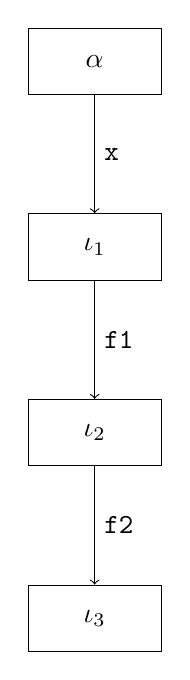
\begin{tikzpicture}[auto,node distance=1.5cm]
    \node[entity] (actor) {$\alpha$};
    \node[entity] (obj1) [below = of actor] {$\iota_1$};
    \node[entity] (obj2) [below = of obj1]  {$\iota_2$};
    \node[entity] (obj3) [below = of obj2]  {$\iota_3$};
    \draw[->] (actor)
        edge	 node {\texttt{x}}    (obj1);
    \draw[->] (obj1)
        edge	 node {\texttt{f1}}	(obj2);
    \draw[->] (obj2)
        edge	 node {\texttt{f2}}	(obj3);
\end{tikzpicture}
        \caption{Chained Field Accesses}
        \label{fig:vis-1}
    \end{subfigure}
    \hfill
    \begin{subfigure}[t]{0.3\textwidth}
        \centering
        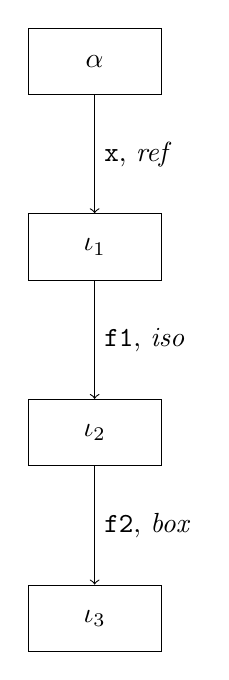
\begin{tikzpicture}[auto,node distance=1.5cm]
    \node[entity] (actor) {$\alpha$};
    \node[entity] (obj1) [below = of actor] {$\iota_1$};
    \node[entity] (obj2) [below = of obj1]  {$\iota_2$};
    \node[entity] (obj3) [below = of obj2]  {$\iota_3$};
    \draw[->] (actor)
        edge	 node {\texttt{x}, \textit{ref}}    (obj1);
    \draw[->] (obj1)
        edge	 node {\texttt{f1}, \textit{iso}}	(obj2);
    \draw[->] (obj2)
        edge	 node {\texttt{f2}, \textit{box}}	(obj3);
\end{tikzpicture}
        \caption{Heap with Explicit Capabilities}
        \label{fig:vis-2}
    \end{subfigure}
    \hfill
    \begin{subfigure}[t]{0.3\textwidth}
        \centering
        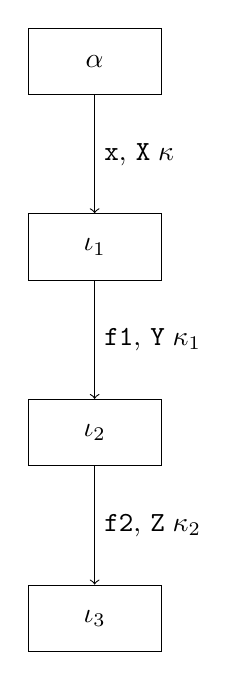
\begin{tikzpicture}[auto,node distance=1.5cm]
    \node[entity] (actor) {$\alpha$};
    \node[entity] (obj1) [below = of actor] {$\iota_1$};
    \node[entity] (obj2) [below = of obj1]  {$\iota_2$};
    \node[entity] (obj3) [below = of obj2]  {$\iota_3$};
    \draw[->] (actor)
        edge	 node {\texttt{x}, $\texttt{X} \; \kappa$}    (obj1);
    \draw[->] (obj1)
        edge	 node {\texttt{f1}, $\texttt{Y} \;\kappa_1$}	(obj2);
    \draw[->] (obj2)
        edge	 node {\texttt{f2}, $\texttt{Z} \;\kappa_2$}	(obj3);
\end{tikzpicture}
        \caption{Heap with Implicit Capabilities}
        \label{fig:vis-3}
    \end{subfigure}
\end{figure}

If the variables and field have the capabilities shown in \ref{fig:vis-2}, the resulting capability of the path \texttt{x.f1.f2} would be $\textit{ref} \triangleright \textit{iso} \triangleright \textit{box}$, giving us a \textit{tag}. However the path \texttt{(x.f1 = y).f2} would have the capability $\textit{ref} \extract \textit{iso} \triangleright \textit{box}$, which is the same as \textit{val}.  \\

Due to the existence of type variables in DeGen, we may not have the capability explicitly available when trying to determine the visibility of a path. For the heap in Figure \ref{fig:vis-3}, where the types of all references are symbolic, we can determine that the path \texttt{x.f1.f2} would have a visibility of $\chi(\alpha)\downarrow_2(\texttt{X}) \triangleright \chi(\iota_1)\downarrow_2(\texttt{Y}) \triangleright \chi(\iota_2)\downarrow_2(\texttt{Z})$. Note that the runtime environments do not actually contain capability information, and we reference them here as something of a shorthand. When determining the visibility of type variable paths, effort must be taken to determine the resulting capability statically. \\

Given the heap and capabilities in \ref{fig:vis-4}, the path \texttt{x.f1.f} has capability \textit{iso}, as does the path \texttt{x.f2.f}. These path visibilities are compatible, since \textit{ref} allows multiple local mutable references, and there is only one \textit{iso} to $\iota_1$. In fact, this heap has well-formed visibility, so any pair of paths is compatible. Note also that the path \texttt{(x = y).f1.f2} has capability $\texttt{this} \extract \textit{iso} \triangleright \textit{ref} \triangleright \textit{ref}$, giving us a visibility of $\textit{iso}^-$, due to the fact that \texttt{this} always has capability \textit{ref} in an actor. 

\begin{figure}[H]
    \centering
    \begin{tikzpicture}[auto,node distance=1.5cm]
    \node[entity] (actor) {$\alpha$};
    \node[entity] (obj1) [below = of actor] {$\iota_1$};
    \node[entity] (obj2) [below left = of obj1]  {$\iota_2$};
    \node[entity] (obj3) [below right = of obj1]  {$\iota_3$};
    \node (blank) [below = of obj1] {};
    \node[entity] (obj4) [below = of blank]  {$\iota_4$};
    \draw[->] (actor)
        edge	 node {\texttt{x}, \textit{iso}}    (obj1);
    \draw[->] (obj1)
        edge	 node {\texttt{f1}, \textit{ref}}	(obj2);
    \draw[->] (obj1)
        edge	 node {\texttt{f2}, \textit{ref}}	(obj3);
    \draw[->] (obj2)
        edge	 node {\texttt{f}, \textit{ref}}	(obj4);
    \draw[->] (obj3)
        edge	 node {\texttt{f}, \textit{ref}}	(obj4);
\end{tikzpicture}
    \caption{Caption}
    \label{fig:vis-4}
\end{figure}

Well-formed visibility is a judgment on the heap, and so we require that all possible pairs of paths are compatible, with each permutation of field access, write, aliasing and unaliasing being valid and well-formed.  

\subsubsection{Proving Well-Formed Visibility}

We would prove that well-formed visibility is preserved much like we would prove soundness, through structural induction over operational semantics; given a heap satisfying well-formed visibility, performing a single execution of a well-typed expression results in a new heap satisfying well-formed visibility, and the type of the expression. By proving it in this manner, we know that the execution of any valid DeGen program has well-formed visibility at all stages of execution, and by extension all well-formed programs are data-race free.

\chapter{Evaluation and Conclusion}

In this section we evaluate DeGen and Genus- relative to the two systems that inspired them, Pony and Genus, and discuss their merits as formal programming models. We discuss some aspects of future work that could be pursued.

\section{In Relation to Pony}

DeGen is a successor to $\textit{Pony}^{PL}$, the formal model of how generics currently exist in Pony. DeGen is designed as an alternative to $\textit{Pony}^{PL}$, showing how a new mechanic for generics can interact with deny capabilities. Since we designed our generic system first, and then applied deny capabilities to it, we have nearly no features that are unrelated to those two aspects. This means that $\textit{Pony}^{PL}$ contains far more features taken from Pony, such as named constructors. It also contains a full runtime description, which DeGen lacks. \\

To evaluate how DeGen compares to Pony, we have taken a portion of the \texttt{List} class from the Pony Standard Library, and recreated it using DeGen. The original portion of \texttt{List} that we are considering is given in Appendix \ref{appendix:list}. Evaluating DeGen in this manner serves a dual purpose; we gain an understanding of how well DeGen can represent Pony programs, and we can also see important features that DeGen lacks. To this end, we have highlighted where it has been necessary to enhance DeGen to accurately recreate the behaviour of \texttt{list}. \\

It is immediate to see that although DeGen represents quite a large subset of Pony features, some necessary mechanisms are still absent. In \texttt{index}, a function which gets the list element at a particular index, Pony uses type coercion to cast \texttt{node} to the desired return type. Viewpoint adaptation always returns a subtype of the operand type, and so here \texttt{this->ListNode[A]} is guaranteed to be compatible with \texttt{ListNode[A]}, the type of \texttt{\_head}. As a result, the method would type check correctly in DeGen even without the cast, but we highlight it here as it is a significant feature that is missing from DeGen. Also missing are various programming constructs such as loops and if-statements, which are highlighted in this example. \\

The function \texttt{map} takes a lambda as a parameter and applies it to every element in a list.  Obviously this is an advanced feature of the language, and is not something we would want to model at this stage, but it serves to demonstrate a level of functionality that DeGen cannot achieve; there is no way to create higher-order functions like \texttt{map} in DeGen. Additionally, it is also interesting to consider the capability the function should have. Since it is being applied in a \textit{box} context, we would expect that it would likely also be a \textit{box} function. The capabilities of its parameter and return types come from the type arguments for \texttt{A} and \texttt{B}, and the type operators that are applied to them. \\

The highlighted elements of Figure \ref{fig:degen-list} suggest aspects of Pony that we would ideally like to have in DeGen. In addition to these, Appendix \ref{appendix:list} demonstrates a number of features of Pony that are interesting, but unnecessary for developing the type system of Genus. There are numerous uses of '\texttt{?}' to indicate partial functions, another advanced language feature that allows Pony to handle errors in a succinct manner. For clarity, we have omitted all error handling from Figure \ref{fig:degen-list}. The syntax '\texttt{.>}' indicates method chaining, where calls to the same object can be combined for brevity. This allows Pony to have a much neater implementation of \texttt{pop}, which in DeGen requires a series of destructive reads to ensure the returned type aliases correctly.

\begin{figure}
    \centering
    \begin{lstlisting}
class List[A #any] {
  ListNode[A] _head;
  ListNode[A] _tail;
  int _size;
  
  ...

  box index(int i) : this->ListNode[A] {
    node = _head (*@\highcode{as this->ListNode[A]}@*);
    
    (*@\highcode{for (int i = 0; i < \_size; i++)}@*) {
      node = node.next() (*@\highcode{as this->ListNode[A]}@*);
    }
    
    return node;
  }
  
  box head() : this->ListNode[A] {
    return _head (*@\highcode{as this->ListNode[A]}@*);
  }
  
  ref push(A a) : (*@\highcode{void}@*) {
    append_node(new ListNode[A](_item = a = null) ref);
  }
  
  ref pop() : A- {
    _size = _size - 1;
    t = _tail = null;
    _tail = t._prev = null;
    return _t = null;
  }
  
  box clone() : List[this->A+]- {
    out = new List[A](_head = null, _tail = null, _size = 0) ref;
    
    (*@\highcode{for (int i = 0; i < \_size; i++)}@*) {
      out.push(this.index(i));
    }
    
    return out;
  }
  
  box map[B #any]((*@\highcode{\{(this->A+) : B-\}}@*) func) : List[B]- {
    return _map[B](_head, 
                   func, 
                   new List[B](_head = null,
                               _tail = null,
                               _size = 0) 
                   ref);
  }

  box _map[B #any](
      this->ListNode[A] last, 
      (*@\highcode{\{(this->A+) : B-\}}@*) func, 
      List[B] acc) : List[B]- {
    acc.push((*@\highcode{func}@*)(ln));
    (*@\highcode{if (ln.next() != null)}@*) {
      _map[B](ln.next() as this->ListNode[A], func, acc);
    } else {
      return acc;
    }
  }
  ...
}

\end{lstlisting}


    \caption{\texttt{list} in DeGen}
    \label{fig:degen-list}
\end{figure}




\section{In Relation to Genus} 

Genus-, and DeGen by extension, present a minimisation of Genus, and so are less expressive by design. However, through this minimisation, we have established a subset of Genus features that we know to be sound.

\begin{itemize}
    \item Our model of Genus- is an imperative model, describing how the state is mutated by the execution of each expression. The formal definition of Genus is not imperative, and so our model is the first description of these behaviours.
    \item Genus does not have a proof of soundness. While the original authors expressed their belief that the system is sound, this project has shown for certain that our distilled formalization is sound. 
    \item Genus- does not contain models as named constructs, instead only using the natural (structural) model of each type. While we have shown in Section \ref{model-just} that our approach to removing models and simplifying Genus is generally valid, we do lose conciseness and some instances of expressiveness, such as expanders and models that take other models as parameters.
    \item Genus- as a programming language is far less expressive system than Genus; Genus, being built on top of Java, is a far more feature-rich system. It also introduces a number of features that do not relate to its mode of generics that increase expressiveness, full existential types being a prime example. We have justified excluding these, but it would be a nice-to-have feature if DeGen is to be developed into a fully fledged programming language.
    
\end{itemize}


\section{Feature Set}

Table \ref{tab:comp} shows how DeGen compares to previous models of Pony and Genus in terms of features. While DeGen does lack a lot of mechanics common to many programming languages, it represents a large subset of relevant features from both Genus and Pony. We note that for both $\textit{Pony}^{PL}$ and DeGen, soundness and data-race freedom are assumed, but not proven; $\textit{Pony}^{PL}$ uses a translation to a non-generic base model, but this translation hasn't been proven sound, and DeGen assumes soundness from Genus- and data-race freedom from the formulation of capabilities in $\textit{Pony}^{GS}$.

\begin{table}[ht]
\centering
\begin{tabular}{l|l|l|l|l|}
\cline{2-5}
                                                              & $\textit{Pony}^{PL}$ & $\textit{Pony}^{GS}$ & Genus       & DeGen \\ \hline
\multicolumn{1}{|l|}{Sound}                                   & \LEFTcircle           & \CIRCLE           &             & \LEFTcircle      \\ \hline
\multicolumn{1}{|l|}{Data-Race Free (Well-Formed Visibility)} & \LEFTcircle           & \CIRCLE           &             & \LEFTcircle      \\ \hline
\multicolumn{1}{|l|}{Actors}                                  & \CIRCLE           & \CIRCLE           &             & \CIRCLE      \\ \hline
\multicolumn{1}{|l|}{Capabilities}                            & \CIRCLE           & \CIRCLE           &             & \CIRCLE      \\ \hline
\multicolumn{1}{|l|}{Destructive Read}                        & \CIRCLE           & \CIRCLE           &             & \CIRCLE      \\ \hline
\multicolumn{1}{|l|}{Recovery}                                & \CIRCLE           & \CIRCLE           &             & \CIRCLE      \\ \hline
\multicolumn{1}{|l|}{Union, Intersection, and Tuple types}    &                      & \CIRCLE           &             &       \\ \hline
\multicolumn{1}{|l|}{Existential Typing}                      &                      &                      & \CIRCLE  &       \\ \hline
\multicolumn{1}{|l|}{Generics}                                & \CIRCLE           &                      & \CIRCLE  & \CIRCLE      \\ \hline
\multicolumn{1}{|l|}{Multiparamter Constraints}               &                      &                      & \CIRCLE  & \CIRCLE      \\ \hline
\multicolumn{1}{|l|}{Multiple Constraints}                    & \CIRCLE           &                      & \CIRCLE  & \CIRCLE      \\ \hline
\multicolumn{1}{|l|}{Natural Models}                          &                      &                      & \CIRCLE  & \CIRCLE      \\ \hline
\multicolumn{1}{|l|}{Parametric Models}                       &                      &                      & \CIRCLE  &       \\ \hline
\multicolumn{1}{|l|}{Retroactive Modelling}                   &                      &                      & \CIRCLE  &       \\ \hline
\multicolumn{1}{|l|}{Model Inheritance}                       &                      &                      & \CIRCLE  &       \\ \hline
\end{tabular}
\caption{Feature Comparison for $\textit{Pony}^{PL}$, $\textit{Pony}^{GS}$, Genus, and DeGen}
\label{tab:comp}
\end{table}

\section{Design Choices}

Throughout the process of minimising Genus and designing DeGen, we made a number of choices that impacted the resulting systems. Here we discuss the choices we made, why we decided to make them, and what impact those choices had.

\subsection{From Genus...}

From the very beginning, our intention when designing Genus- was to create as simple a system as possible that had the same generic mechanism as Genus, while also maintaining enough expressiveness to allow us to reintroduce deny capabilities. \\

We opted to create an imperative model rather than just a standalone type system. With our intention being to prove well-formed visibility, a judgement on the heap, when we reintroduced capabilities, we knew the model would need a runtime specification eventually. Upon reflection, it was not necessary to introduce the runtime system while we still only had Genus-; Genus itself is not an imperative model, and a large part of the early stages on this project focused on creating this imperative model and proving its soundness. Had we instead focused on cherry-picking the aspects of Genus we wanted and then introduced the runtime specification when we introduce capabilities, we may have had time to fully develop the imperative model of DeGen. \\

A significant first step to our simplification of Genus was the decision to remove interfaces from the language entirely. Interfaces are used in examples in \cite{Zhang2015}, but the formal specification does not reference them at all. Our intuition told us they were unnecessary, due to the fact that interfaces in most programming languages and constraints in Genus play nearly equivalent roles. We created a translation, described in \ref{sec:translation} that showed this to be true, and that any interface declaration can be replaced by an equivalent constraint. However, there was a slight oversight in our reasoning that is demonstrated in Figure \ref{fig:degen-varbox}; unlike interfaces in other languages, we do not allow constraints to be used as types, and so they cannot be used as type arguments. This affects the case where we wish to apply binary functions to two different types which obey the same constraint. \\

Once we decided we were going to remove interfaces, the next step was deciding how we would replace the behaviour they represent; we knew from our translation that we could replace interfaces as constraints, but it required us to augment the behaviour of constraints in a non-intuitive way. Interfaces such as \texttt{Set[A]} can only be represented by constraints in a meaningful way if we allowed the type variables that constraints act on to themselves be constrained. However, for constraints to properly act as predicates, constrained type variables can't be used as receivers. Section \ref{sec:mat-wit} gives an approach to witnessing that enabled us to reason about how we can manifest these requirements, with parametric constraints becoming either functions returning constraints (in the manner that parametric classes are commonly thought of), or multivariate predicates that impose conditions on their type variables. We opted to keep a single list of type variables for constraints and more complicated type rules, but upon reflection, it would have been more desirable to slightly simplify the type system, even at the cost of a messier syntax. \\

The most significant decision we made concerning the minimisation of Genus was to remove models. Models supply a large part of the expressiveness of Genus, and so we carefully considered the implications of removing them; by the formulation in Section \ref{sec:mat-wit}, we knew the natural model of each type was sufficient to witness a constraint, and so we could . However, since a significant motivation for reformulating generics using Genus was reducing programmer burden, we wanted to ensure that removing models did not greatly increase the complexity of using Genus. Section \ref{model-just} represents a principled analysis of the features that we lose as a result of removing models, and how we can replace that behaviour. Not all behaviour can be recreated succinctly, such as parametric models, but there is not a significant increase in overall complexity. \\

We initially started developing Genus- with existentially qualified types, but chose to remove them based on the complexity they added to the type system. Genus expands the functionality of use-site genericity far beyond what Java wildcards are capable of. However, the complexity of existential packing and capture conversion that existential type require outweighed their usefulness. Section \ref{sec:genus-types} provides justification for their removal with reference to the equivalence between universal and existential types. 

\subsection{...to DeGen}

After establishing Genus- as a sound base upon which we could further develop a more complex type system, the next step was to design how we would incorporate deny capabilities into Genus-. Since we intended DeGen to be an illustrative exploration of an alternate system of generics to the one that currently exists in Pony, we knew that DeGen must have the same system of concurrency as Pony, that of actors and messaging. Again for simplicity, we chose to model the smallest subset of features that accurately represent the deny capability system. We therefore don't introduce any features of Pony that do not relate to either actor-based execution or well-formed visibility. \\

We undertook a design process to understand how capabilities interact with type variables in Pony by recreating the behaviour of a number of Genus- constraints, which we detail in Section \ref{pony-degen}. As a result of this principled analysis, which allowed us to reason about and understand the required capabilities of a number of constraints, we developed an idea of how capabilities should interact with constraints and type variables. \\

The aspect of the design that required the most consideration was how we apply capabilities to constraints. We discovered that the simplest solution was also the most intuitive; constraints act as predicates on types that define the expected behaviour of those types. By extending this idea, it becomes clear that constraints can be used not only to say what a type can do, but also what we can do to the type. Type variables, therefore, should define what the program is permitted to do to a reference of that type. For example, the constraint \texttt{Box[B, T]} as defined in Figure \ref{fig:degen-varbox} requires that a witness must have \texttt{get} and \texttt{set} methods, and that its type argument \texttt{T} is immutable. We also allow capability constraints to be placed on the 'self' type variables. This design choice allows the programmer to require that the witnesses of certain constraints are, for example, sendable, if that was the intention of the constraint. \\



\chapter{Conclusion}

This project has shown that deny capabilities and constraint-based generics can be combined into a succinct formal specification that is likely sound and data-race free. This system alleviates the programmer burden caused by f-bounded polymorphism and empowers them to use generics in a simple, intuitive way.  \\

Over the course of the project, we have focused our efforts on ensuring the systems we are building are well designed. We have justified each design decision, and they have resulted in two concise, simple models. Being guided by this principled design approach allowed us to iterate quickly on design ideas, and, in nearly all cases, know quickly when we were pursuing ineffective avenues of design. \\

\section{Future Work}

DeGen is currently a very simple system, and so there are many possible avenues of future work, many of which we discussed in the previous chapter. We mention just some of these here:

\begin{itemize}
    \item Expand DeGen into a full formal model, including runtime specification and operational semantics, and show that it preserves both soundness and well-formed visibility. Once these properties have been proven, we will have established DeGen as a valid proof of concept for constraint bounded generics in an actor-based language.
    \item Both Pony and Genus support features that DeGen does not. A key aspect to developing DeGen further would be to reintroduce some of these features in order to add greater expressiveness and power to the system. For example, adding Genus models as named constructs to DeGen would allow us to fully utilise the expressive power of using constraints and models in conjunction.
    \item A DeGen compiler would allow DeGen to form the basis for future programming language implementations, whether it be a new major version of Pony supporting constraint generics, or a spiritual successor to Pony.
\end{itemize}


\bibliographystyle{unsrt}
\bibliography{bibs/ProjectBackground}

\appendix
\chapter{Genus- Model} \label{appendix:genusminus}

\section{Syntax}

\begin{figure}[H]
    \centering
    \begin{align*}
        &Programs & \texttt{P} &::= \overline{\texttt{CO}} \: \overline{\texttt{CL}} \\
        &Constraints & \texttt{CO} &::= \texttt{constraint} \: C_1[\overline{\texttt{X}} \; \texttt{where} \; \overline{C_2[\overline{\texttt{Y}}]}] \: \texttt{extends} \: C_3[\overline{\texttt{Z}}] \; \{ \overline{\texttt{methSig}} \} \\
        &Classes & \texttt{CL} &::= \texttt{class} \: L_1[\beta] \: \texttt{extends} \: L_2[\overline{\tau}] \; \{ \overline{\texttt{fld}} \: \overline{\texttt{meth}} \} \\
        &Method \; Signature & \texttt{methSig} &::= \tau_1 \: \tau_2.m[\beta](\overline{\tau_3}) \\
        &Method \; Declaration & \texttt{meth} &::= \texttt{methSig} \; \{ \texttt{e}\} \\
        &Field \; Declaration & \texttt{fld} &::= \tau \; f \\
        &Generic \; Parameters & \beta &::= \overline{\texttt{X}} \: \texttt{where} \: \overline{C[\overline{\tau}]} \\
        &Types & \tau &::= \texttt{X} \: | \: L[\overline{\tau}] \\
        &Expressions & \texttt{e} &::= x \; | \; \texttt{e}.f \; | \; \texttt{e}.f \: = \: \texttt{e} \; | \; \texttt{this} \; | \; \texttt{new} \: L[\overline{\tau}]( \overline{f = \texttt{e}} ) \; | \; \texttt{e}.m[\overline{\tau_2}](\overline{\texttt{e}}) \\
        &Type \; Environments & \Gamma &::= \overline{\texttt{X}} \\
        &Constraint \; Environments & \Delta &::= \overline{C[\overline{\texttt{X}}]} \\
        &Value \; Environments & E &::= \emptyset \; | \; E, x : \tau \; | \; E, \texttt{this} : \tau 
    \end{align*}
    \begin{align*}
        &Constraint \: Names & &C & &Class \: Names & &L \\
        &Method \: Names & &m & &Field \: Names & &f \\
        &Variable \: Names & &x & &Type \: Variables & &\texttt{X}
    \end{align*}
    \caption{Syntax}
    \label{fig:G-Syntax}
\end{figure}
\newpage

\section{Interface to Constraint Translation}\label{appendix:intertrans}

\begin{figure}[H]
    \centering
    \begin{align*}
        &Interface \; Declaration & \texttt{I} &::= \texttt{interface} \; I\langle{\texttt{X}} \; \texttt{where} \; \overline{C[\overline{\texttt{Y}}]}\rangle \{ \overline{\Dot{\tau_1} \: m[\beta](\overline{\Dot{\tau_2}})} \} \\
        &Programs & \texttt{P} &::= \overline{\texttt{CO}} \: \overline{\texttt{CL}} \: \overline{\texttt{I}} \\
        &Interface \; Types & \Dot{\tau} &::= \tau \: | \: I\langle\overline{\Dot{\tau}}\rangle \\
        &Method \; Signature & \texttt{methSig} &::= \Dot{\tau_1} \: \tau_2.m[\beta](\overline{\Dot{\tau_3}})
    \end{align*}
    \caption{Interface Syntax}
    \label{fig:interface-syntax}
\end{figure}

\begin{figure}[H]
    \centering
    \begin{align*}
       &expand :: I\langle\overline{\Dot{\tau}}\rangle \times \Gamma \; \to \; \overline{\texttt{X}} \times \overline{C[\overline{\tau}}] \\
       &expand(I\langle\overline{\tau}\rangle, \Gamma) = (\texttt{U}, \; C_I[\texttt{U}, \overline{\tau}]) \quad \texttt{where U new in } \Gamma  \\
       &expand(I\langle\overline{\Dot{\tau}}\rangle, \Gamma) = (\texttt{U}:\overline{\texttt{U}'}:\overline{us}, \; C_I[\texttt{U},  \overline{\texttt{U}'}]:\overline{cs}) \\
       &\quad\quad\quad \texttt{where U new in } \Gamma \land \forall i \; . \; expand(\Dot{\tau}_i, \Gamma:\texttt{U}) = (\texttt{U}'_i:us_i, \; cs_i) \\
       &\quad\quad\quad us :: \overline{\texttt{X}}, \; cs :: \overline{C[\overline{\tau}]}
    \end{align*}
    \caption{Definition of \textit{expand} function}
    \label{fig:interface-expand}
\end{figure}

\begin{figure}[H]
    \centering
    \begin{mathpar}
        \inferrule[T-Prog]{\forall i \; . \; \texttt{CO}_i \rightsquigarrow^T \texttt{CO}'_i \\\\
        \forall j \; . \; \texttt{CL}_j \rightsquigarrow^T \texttt{CL}'_j \\\\
        \forall k \; . \; \texttt{I}_k \rightsquigarrow^T \texttt{CO}'_{i+k}}{\texttt{P} \rightsquigarrow^T \overline{\texttt{CO}'} \: \overline{\texttt{CL}'}}
        \and
        \inferrule[T-Interface]{I \rightsquigarrow^T C_I \\\\
        \texttt{constraint} \; C_I[\texttt{S}, \overline{\texttt{X}} \; \texttt{where} \; \overline{C[\overline{\texttt{Y}}]}] \{ \overline{\Dot{\tau_1} \: \texttt{S}.m[\beta](\overline{\Dot{\tau_3}})} \} \rightsquigarrow^T c  }{\texttt{interface} \; I\langle\overline{\texttt{X}} \; \texttt{where} \; \overline{C[\overline{\texttt{Y}}]}\rangle \{ \overline{\Dot{\tau_1} \: m[\beta](\overline{\Dot{\tau_2}})} \} \rightsquigarrow^T c}
        \and
        \inferrule[T-Ident]{C_I = `c\_` + I}{I \rightsquigarrow^T C_I}
        \and
        \inferrule[T-Meth]{\forall i \; . \; expand(I\langle\overline{\Dot{\tau}}\rangle_i, \Gamma:\overline{\texttt{X}}) =  (\texttt{U}_i : us_i, cs_i)}{\tau_1 \: \tau_2.m[\overline{\texttt{X}} \; \texttt{where} \; \overline{C[\overline{\texttt{Y}}]}](\overline{\tau_3}, \overline{I\langle\overline{\tau}\rangle}), \Gamma \rightsquigarrow^T \tau_1 \: \tau_2.m[\overline{\texttt{X}}, \overline{\texttt{U}}, \overline{us} \; \texttt{where} \; \overline{C[\overline{\texttt{Y}}]}, \overline{cs}](\overline{\tau_3}, \overline{\texttt{U}})}
        \and
        \inferrule[T-Constraint]{\forall i \; . \; expand(I\langle\overline{\Dot{\tau}}\rangle_i, \overline{\texttt{X}}) =  (\texttt{U}_i : us_i, cs_i) \\\\
        \forall i \; . \; (\texttt{U}_i \; (\tau_2.m[\beta](\overline{\Dot{\tau_3}}))_i, \overline{\texttt{X}}:\overline{\texttt{U}}:\overline{us} \rightsquigarrow^T \texttt{meth}_i) \\\\
        \forall j \; . \; ((\tau_4 \: \tau_3.m[\beta](\overline{\Dot{\tau_6}}))_j, \overline{\texttt{X}}:\overline{\texttt{U}}:\overline{us} \rightsquigarrow^T \texttt{meth}_{i+j})}{\texttt{constraint} \: C_1[\overline{\texttt{X}} \; \texttt{where} \; \overline{C[\overline{\texttt{Y}}]}] \: \texttt{extends} \: C_2[\overline{\texttt{Z}}] \; \{ \overline{I\langle\overline{\Dot{\tau}}\rangle \: \tau_2.m[\beta](\overline{\Dot{\tau_3}})}, \overline{\tau_4 \; \tau_5.m[\beta](\overline{\Dot{\tau_6}})} \} \rightsquigarrow^T \\\\ \texttt{constraint} \: C_1[\overline{\texttt{X}}, \overline{\texttt{U}}, \overline{us} \; \texttt{where} \; \overline{C[\overline{\texttt{Y}}]}, \overline{cs}] \: \texttt{extends} \: C_2[\overline{\texttt{Z}}] \; \{\overline{\texttt{meth}}\}}
        \and
        \inferrule[T-Class]{\forall i \; . \; expand(I\langle\overline{\Dot{\tau}}\rangle_i, \overline{\texttt{X}}) =  (\texttt{U}_i : us_i, cs_i) \\\\
        \forall i \; . \; (\texttt{U}_i \; (\tau_2.m[\beta](\overline{\Dot{\tau_3}}) \; \{\texttt{e}\})_i, \overline{\texttt{X}}:\overline{\texttt{U}}:\overline{us} \rightsquigarrow^T \texttt{meth}_i) \\\\
        \forall j \; . \; ((\tau_4 \: \tau_3.m[\beta](\overline{\Dot{\tau_6}}) \; \{\texttt{e}\})_j, \overline{\texttt{X}}:\overline{\texttt{U}}:\overline{us} \rightsquigarrow^T \texttt{meth}_{i+j})}{\texttt{class} \: L_1[\overline{\texttt{X}} \; \texttt{where} \; \overline{C[\overline{\texttt{Y}}]}] \: \texttt{extends} \: L_2[\overline{\tau}] \; \{\overline{\texttt{fld}}, \; \overline{I\langle\overline{\Dot{\tau}}\rangle \: \tau_2.m[\beta](\overline{\Dot{\tau_3}}) \; \{\texttt{e}\}}, \overline{\tau_4 \; \tau_5.m[\beta](\overline{\Dot{\tau_6}}) \; \{\texttt{e}\}} \} \rightsquigarrow^T \\\\ \texttt{class} \: L_1[\overline{\texttt{X}}, \overline{\texttt{U}}, \overline{us} \; \texttt{where} \; \overline{C[\overline{\texttt{Y}}]}, \overline{cs}] \: \texttt{extends} \: L_2[\overline{\tau}] \; \{\overline{\texttt{fld}}, \; \overline{\texttt{meth}}\}}
        \and
        \inferrule[T-MethDecl]{\texttt{meth}, \Gamma \rightsquigarrow \texttt{meth}'}{\texttt{meth} \; \{\texttt{e}\}, \Gamma \rightsquigarrow \texttt{meth}'  \; \{\texttt{e}\}}
    \end{mathpar}
    \caption{Translation Rules}
    \label{fig:interface-translation}
\end{figure}

\newpage

\section{Well-formed Programs} \label{appendix:genus-wf}

\begin{figure}[H]
    \centering
    \begin{mathpar}
        \inferrule[L-Cons]{Prog = {\overline{\texttt{CO}} \: \overline{\texttt{CL}}} }{Constraints(Prog) = \overline{\texttt{CO}}}
        \and
        \inferrule[L-Classes]{Prog = {\overline{\texttt{CO}} \: \overline{\texttt{CL}}} }{Constraints(Prog) = \overline{\texttt{CL}}}
        \and
        \inferrule[L-Con]{Constraints(Prog)_i = \texttt{constraint} \; C \; ... \; \{ ... \} }{Constraint(Prog, C) = Constraints(Prog)_i }
        \and
        \inferrule[L-Class]{ Classes(Prog)_i = \texttt{class} \; L \; ... \; \{ ... \} }{Class(Prog, L) = Classes(Prog)_i }
        \and
        \inferrule[L-F-L]{Class(Prog, L) = \texttt{class} \; L[\overline{\texttt{X}} \; ...] \; ... \; \{ ... \; \tau \; f \; ...\} }{Field(Prog, L[\overline{\tau}], f) = \tau\{\overline{\tau}/\overline{\texttt{X}}\} }
        \and`
        \inferrule[L-Fs-L]{Class(Prog, L) = \texttt{class} \; L \; ... \; \{\overline{\tau \: f} \; ...\}}{Fields(Prog, L) = \overline{f}}
        \and
        \inferrule[L-Funcs-Con]{Constraint(Prog, C) = \texttt{constraint} \; C[\overline{\texttt{X}} \; ...] \; \texttt{extends} \; C'[...] \; \{ {\overline{\texttt{methSig}}}\} \\\\ Funcs(Prog, C') = \overline{m}}{Funcs(Prog, \Delta, C[\overline{\tau}]) = \overline{\texttt{methSig}}\{\overline{\tau}/\overline{\texttt{X}}\}, \overline{m}\{\overline{\tau}/\overline{\texttt{X}}\}}
        \and
        \inferrule[L-Funcs-Class]{Class(Prog, L) = \texttt{class} \; L[\overline{\texttt{X}} \; ...] \; \texttt{extends} \; L'[...] \; \{... \; {\overline{\texttt{methSig} \; \{\texttt{e}\}}}\} \\\\ Funcs(Prog, L') = \overline{m}}{Funcs(Prog, \Delta, L[\overline{\tau}]) = \overline{\texttt{methSig}}\{\overline{\tau}/\overline{\texttt{X}}\}, \overline{m}\{\overline{\tau}/\overline{\texttt{X}}\}}
        \and
        \inferrule[L-Funcs-Var]{ \overline{C} = \{ C | C[\overline{\texttt{X'}}, \texttt{X}, \overline{\texttt{X''}}] \in \Delta \} \\\\
        \overline{\texttt{mSig}} = \{ \texttt{mSig} \; | \; \exists C \in \overline{C}, \tau, \overline{\tau} \; . \; \texttt{mSig} \in Func(Prog, \Delta, C) \land \texttt{mSig} = \tau \; \texttt{X}.m(\overline{\tau}) \}
        }{Funcs(Prog, \Delta, \texttt{X}) = \overline{\texttt{mSig}}}
        \and
        \inferrule[L-Func]{Funcs(Prog, \Delta, \tau) = \overline{m} \\\\
        m_i = \tau_1 \; \tau_2.m[\beta](\overline{\tau_3})}{Func(Prog, \Delta, \tau, m) = m_i }
        \and
        \inferrule[L-M-Body]{Class(Prog, L) = \texttt{class} \; L[...] \; ... \; \{... \; \tau' \; \tau''.m[\overline{\texttt{X}} \; \texttt{where} \; \overline{C[\overline{\tau'''}]}](\overline{\tau'''' \; x})\{ \texttt{e} \} \; ... \}}{Meth(Prog, L, m) = \tau' \; \tau''.m[\overline{\texttt{X}} \; \texttt{where} \; \overline{C[\overline{\tau'''}]}](\overline{\tau'''' \; x})\{ \texttt{e} \}}
    \end{mathpar}
    \caption{Lookup Functions}
    \label{fig:genus-lookup}
\end{figure}

\begin{figure}[H]
    \centering
    \begin{mathpar}
        \inferrule[S-Refl]{ }{Prog \vdash \tau \leq \tau}
        \and
        \inferrule[S-Trans]{Prog \vdash \tau_1 \leq \tau_2 \\ Prog \vdash \tau_2 \leq \tau_3}{Prog \vdash \tau_1 \leq \tau_3}
        \and
        \inferrule[S-Subclass]{ Class(Prog, L_1) = \texttt{class} \; L_1[\overline{\texttt{X}}] \; \texttt{extends} \; L_2[\overline{\tau_2}] \; \{ ... \} }{Prog\vdash L_1[\overline{\tau_1}] \leq L_2[\overline{\tau_2}\{\overline{\tau_1} / \overline{\texttt{X}} \}]}
        \and
        \inferrule[S-Object]{ }{Prog; \Gamma \vdash \tau \leq \textit{Object}}
    \end{mathpar}
    \caption{Subtyping Rules}
    \label{fig:genus-subtyping}
\end{figure}

\begin{figure}[H]
    \centering
    \begin{mathpar}
    \inferrule[E-Prereq]{Constraint(Prog, C_1) = \texttt{constraint} \; C_1[\overline{\texttt{X}_1}] \; \texttt{extends} \; C_2[\overline{\texttt{X}_2}] \; \{...\} }{Prog \vdash C_1[\overline{\tau}] \preceq C_2[\overline{\texttt{X}_2}\{\overline{\tau}/\overline{\texttt{X}_1}\}]}
    \and
    \inferrule[E-Trans]{Prog \vdash C_1[\overline{\tau_1}] \preceq C_2[\overline{\tau_2}] \\ Prog \vdash C_1[\overline{\tau_2}] \preceq C_2[\overline{\tau_3}]}{Prog \vdash C_1[\overline{\tau_1}] \preceq C_2[\overline{\tau_3}]}
    \and
    \inferrule[E-Reflex]{ }{Prog \vdash C[\overline{\tau}] \preceq C[\overline{\tau}]}
    \end{mathpar}
    \caption{Constraint Entailment}
    \label{fig:genus-ce}
\end{figure}

\begin{figure}[H]
    \centering
    \begin{mathpar}
    \inferrule[W-Subsume]{Prog; \Delta \vdash \overline{\tau} :: C_1[\overline{\tau_1}] \\ Prog \vdash C_1[\overline{\tau_1}] \preceq C_2[\overline{\tau_2}]}{Prog; \Delta \vdash \overline{\tau} :: C_2[\overline{\tau_2}]}
    \and
    \inferrule[W-Class]{Funcs(Prog, \Delta, C[\overline{\tau}]) \subseteq \bigcup_i Funcs(Prog, \Delta, \tau_i)}{Prog; \Delta \vdash \overline{\tau} :: C[\overline{\tau}]}
    \end{mathpar}
    \caption{Witness Relation}
    \label{fig:genus-witness}
\end{figure}

\begin{figure}[H]
    \centering
    \begin{mathpar}
        \inferrule[W-Prog]{\forall C \in Constraints(Prog) \: . \: Prog \vdash C : \texttt{ok} \\\\
        \forall L \in Classes(Prog) \: . \: Prog \vdash L : \texttt{ok} }{\vdash Prog : \texttt{ok}}
    \end{mathpar}
    \caption{Well-formed Programs}
    \label{fig:genus-wfp}
\end{figure}

\begin{figure}[H]
    \centering
    \begin{mathpar}
        \inferrule[W-CDecl]{ \overline{\texttt{X}_2} \subseteq \overline{\texttt{X}_1} \\ \overline{\texttt{X}_3} \subseteq \overline{\texttt{X}_1} \\\\
        \forall i \: . \: Prog; \overline{\texttt{X}_1}; \emptyset \vdash C_2[\overline{\texttt{X}_2}]_i : \texttt{ok} \\ Prog; \overline{\texttt{X}_1}; \emptyset \vdash C_3[\overline{\texttt{X}_3}] : \texttt{ok} \\\\
        \forall i \: . \: Prog; \: \overline{\texttt{X}_1}; \overline{C_2[\texttt{X}_2]}, C_3[\texttt{X}_3] \vdash (\tau_1 \: \tau_2.m[\beta](\overline{\tau_3}))_i : \texttt{ok} \\ \forall i . \exists j \: . \: (\tau_2)_i = (\texttt{X}_1)_j \land (\texttt{X}_1)_j \notin \overline{\texttt{X}_2}}{Prog \vdash \; \texttt{constraint} \: C_1[\overline{\texttt{X}_1} \: \texttt{where} \: \overline{C_2[\overline{\texttt{X}_2}}]] \: \texttt{extends} \: C_3[\overline{\texttt{X}_3}] \; \{ \overline{\tau_1 \: \tau_2.m[\beta](\overline{\tau_3})} \} : \texttt{ok} }
    \end{mathpar}
    \caption{Well-Formed Constraint Declarations}
    \label{fig:genus-wfc}
\end{figure}

\begin{figure}[H]
    \centering
    \begin{mathpar}
        \inferrule[W-LDecl]{\forall i \: . \: Prog; \overline{\texttt{X}}; \emptyset \vdash C[\overline{\tau_1}]_i : \texttt{ok} \\ Prog; \overline{\texttt{X}}; \emptyset \vdash L[\overline{\tau_2}] : \texttt{ok} \\ \forall i \; . \; Prog; \overline{\texttt{X}}; \overline{C[\overline{\tau_1}]} \vdash (\tau_f)_i : \texttt{ok} \\\\ 
        \forall i \: . \: Prog; \overline{\texttt{X}}; \overline{C[\overline{\tau_1}]} \vdash (\tau_3 \: \tau_4.m[\beta](\overline{\tau_5})\{\texttt{e}\})_i : \texttt{ok} \\ \forall i \: . \: Prog; \overline{\texttt{X}}; \overline{C[\overline{\tau_1}]} \vdash (\tau_4)_i : L_1[\overline{\texttt{X}}] \\\\
        (\exists j \; . \; Funcs(Prog, L_2)_j = \tau_3' \; \tau_4'.m[\beta](\overline{\tau_5'})) \implies \tau_3 = \tau_3' \land \forall k \; . \; (\tau_5)_k = (\tau_5')_k}{Prog \vdash \: \texttt{class} \: L_1[\overline{\texttt{X}} \: \texttt{where} \: \overline{C[\overline{\tau_1}}]] \: \texttt{extends} \:  L_2[\overline{\tau_2}] \{\overline{\tau_f \; f} \; \overline{\tau_3 \: \tau_4.m[\beta](\overline{\tau_5})\{\texttt{e}\}} \} : \texttt{ok} }
    \end{mathpar}
    \caption{Well-Formed Class Declarations}
    \label{fig:genus-wfl}
\end{figure}

\begin{figure}[H]
    \centering
    \begin{mathpar}
        \inferrule[W-MethSig]{Prog; \Gamma; \Delta \vdash \tau_1 : \texttt{ok} \\ Prog; \Gamma; \Delta \vdash \tau_2 : \texttt{ok} \\\\
        \forall i \; . \; Prog; \Gamma, \overline{\texttt{X}}; \Delta, \overline{C[\overline{\tau}]} \vdash (\tau_3)_i : \texttt{ok} \\ \forall i \; . \; Prog; \Gamma, \overline{\texttt{X}}; \Delta \vdash (C[\overline{\tau}])_i : \texttt{ok}}{Prog; \Gamma; \Delta \vdash \tau_1 \; \tau_2.m[\overline{\texttt{X}} \; \texttt{where} \; \overline{C[\overline{\tau}]}](\overline{\tau_3}) : \texttt{ok}}
        \and
        \inferrule[W-MethDecl]{Prog; \Gamma; \Delta \vdash \tau_1 \; \tau_2.m[\overline{\texttt{X}} \; \texttt{where} \; \overline{C[\overline{\tau}]}](\overline{\tau_3}) : \texttt{ok} \\\\
        Prog; \Gamma, \overline{\texttt{X}}; \Delta, \overline{C[\overline{\tau}]}; \texttt{this} : \tau_2, \overline{x : \tau_3} \vdash \texttt{e} : \tau_1}{Prog; \Gamma; \Delta \vdash \tau_1 \; \tau_2.m[\overline{\texttt{X}} \; \texttt{where} \; \overline{C[\overline{\tau}]}](\overline{\tau_3 \; x}) \; \{ \texttt{e} \} : \texttt{ok}}
    \end{mathpar}
    \caption{Well-Formed Methods}
    \label{fig:genus-wfm}
\end{figure}

\begin{figure}[H]
    \centering
    \begin{mathpar}
        \inferrule[W-TVar]{\texttt{X} \in \Gamma}{Prog; \Gamma; \Delta \vdash \texttt{X} : \texttt{ok}}
        \and
        \inferrule[W-TL]{Class(Prog, L) = \texttt{class} \: L[\overline{\texttt{X}} \: \texttt{where} \: \overline{C[\overline{\tau_2}}]] \: \texttt{extends} \:  L_2[\overline{\tau_3}] \{...\} \\\\
        \forall i \: . \: Prog; \Gamma; \Delta \vdash (\tau_1)_i : \texttt{ok} \\ \#(\overline{\tau_1}) = \#(\overline{\texttt{X}}) \\\\
        Prog; \Gamma, \overline{\texttt{X}}; \Delta \vdash L_2[\overline{\tau_3}\{\overline{\tau_1}/\overline{\texttt{X}}\}] : \texttt{ok} \\ \forall i \; . \; Prog; \Gamma, \overline{\texttt{X}}; \Delta \vdash C[\overline{\tau_2}\{\overline{\tau_1}/\overline{\texttt{X}}\}]_i : \texttt{ok} \\\\
        \forall i \; . \; Prog; \Gamma; \Delta \vdash (\overline{\tau_2} \{\overline{\tau_1}/\overline{\texttt{X}}\})_i :: C[\overline{\tau_2} \{\overline{\tau_1}/\overline{\texttt{X}}\}]_i}{Prog; \Gamma; \Delta \vdash L[\overline{\tau_1}] : \texttt{ok}}
        \and
        \inferrule[W-TC]{Constraint(Prog, C) = \texttt{constraint} \: C[\overline{\texttt{X}} \: \texttt{where} \: \overline{C_2[\overline{\texttt{Y}}}]] \: \texttt{extends} \:  C_3[\overline{\texttt{Z}}] \{...\} \\\\
        \forall i \: . \: Prog; \Gamma; \Delta \vdash \tau_i : \texttt{ok} \\ \#(\overline{\tau}) = \#(\overline{\texttt{X}}) \\\\
        \forall i \; . \; Prog; \Gamma, \overline{\texttt{X}}; \Delta \vdash C_2[\overline{\texttt{Y}}\{\overline{\tau}/\overline{\texttt{X}}\}]_i : \texttt{ok}  \\ Prog; \Gamma, \overline{\texttt{X}}; \Delta \vdash C_3[\overline{\texttt{Z}}\{\overline{\tau}/\overline{\texttt{X}}\}] : \texttt{ok} \\\\
        \forall i \; . \; Prog; \Gamma; \Delta \vdash (\overline{\texttt{Y}} \{\overline{\tau}/\overline{\texttt{X}}\})_i :: C_2[\overline{\texttt{Y}} \{\overline{\tau}/\overline{\texttt{X}}\}]_i}{Prog; \Gamma; \Delta \vdash C[\overline{\tau}] : \texttt{ok}}
    \end{mathpar}
    \caption{Well-Formed Types and Constraints}
    \label{fig:genus-wft}
\end{figure}

\begin{figure}[H]
    \centering
    \begin{mathpar}
        \inferrule[var-x]{ }{Prog; \Gamma; \Delta; E \vdash x : E(x)}
        \and
        \inferrule[var-this]{ }{Prog; \Gamma; \Delta; E \vdash \texttt{this} : E(\texttt{this})}
        \and
        \inferrule[fld]{Prog; \Gamma; \Delta; E \vdash e : L[\overline{\tau_1}] \\\\
        Class(Prog, L) = \texttt{class} \: L[\overline{\texttt{X}}] \: ... \: \{... \: \tau_2 \: f \: ...\}}{Prog; \Gamma; \Delta; E \vdash e.f : \tau_2\{\overline{\tau_1}/\overline{\texttt{X}}\}}
        \and
        \inferrule[fld-ass]{Prog; \Gamma; \Delta; E \vdash e_1.f : \tau \\\\
        Prog; \Gamma; \Delta; E, \vdash e_2 : \tau}{Prog; \Gamma; \Delta; E \vdash e_1.f = e_2 : \tau}
        \and
        \inferrule[new]{Prog; \Gamma \vdash L[\overline{\tau_1}] : \texttt{ok} \\\\
        \forall i \: . \: Prog; \Gamma; \Delta; E \vdash \texttt{e}_i: Field(Prog, L[\overline{\tau_1}], f_i) \\\\
        \overline{f} = Fields(Prog, L)}{Prog; \Gamma; \Delta; E \vdash \texttt{new} \: L[\overline{\tau_1}](\overline{f = \texttt{e}}) : L[\overline{\tau_1}]}
        \and
        \inferrule[m-call]{Prog; \Gamma; \Delta; E \vdash \texttt{e}_1 : \tau_1  \\ \forall i \: . \: Prog; \Gamma \vdash (\tau_2)_i : \texttt{ok} \\\\
        Func(Prog, \Delta, \tau_1, m) = \tau_3 \; \tau_1.m[\overline{\texttt{X}} \; \texttt{where} \; \overline{C[\overline{\tau_5}]}](\overline{\tau_4})\\\\
        \forall i \; . \; Prog; \Gamma; \Delta; E \vdash (\texttt{e}_4)_i : (\tau_4\{\overline{\tau_2}/\overline{\texttt{X}}\})_i \\\\
         \forall i \; . \; Prog; \Delta \vdash (\overline{\tau_5} \{\overline{\tau_2}/\overline{\texttt{X}}\})_i :: C[\overline{\tau_5} \{\overline{\tau_2}/\overline{\texttt{X}}\}]_i}{Prog; \Gamma; \Delta; E \vdash \texttt{e}_1.m[\overline{\tau_2}](\overline{\texttt{e}_4}) : \tau_3}
        \and
        \inferrule[Subsumption]{Prog; \Gamma; \Delta; E \vdash \texttt{e} : \tau_1 \\\\
        Prog \vdash \tau_1 \leq \tau_2}{Prog; \Gamma; \Delta; E \vdash \texttt{e} : \tau_2}
    \end{mathpar}
    \caption{Well-Formed Expressions}
    \label{fig:genus-wfe}
\end{figure}

\newpage

\section{Runtime Specification} \label{sec:genus-rs}

\begin{figure}[H]
    \centering
    \begin{align*}
        &\chi & &\in & &Heap & &= Addr \to Object \\
        &\phi & &\in & &StackFrame & &= Addr \times \Omega \times (VarId \mapsto Value) \\
        &\iota & &\in & &Addr & & \\
        &v & &\in & &Value & &= Addr \\
        & & & & &Object & &= ClassId \times \Omega \times (FieldId \mapsto Value) \\
        &\Omega & &\in & &RuntimeEnv & &= \texttt{X} \mapsto \sigma \\
        &\sigma & &\in & &ConcreteType & &= L[\overline{\sigma}]
    \end{align*}
    \caption{Runtime Entities}
    \label{fig:genus-runent}
\end{figure}

\begin{figure}[h]
    \centering
    \begin{align*}
    &resolve :: \tau \times \Omega \to \sigma \\
    &resolve(\texttt{X}, \Omega) = \Omega(\texttt{X}) \\
    &resolve(L[\overline{\tau}], \Omega) = L[\overline{resolve(\tau)}]
    \end{align*}
    \caption{Resolve Function}
    \label{fig:genus-resolve}
\end{figure}

\begin{figure}[H]
    \centering
    \begin{mathpar}
    \inferrule[val]{v \; \in \; Value}{v, \phi, \chi \rightsquigarrow_P v, \chi}
    \and
    \inferrule[this]{ }{\texttt{this}, (\iota, \Omega, \texttt{vMap}), \chi \rightsquigarrow_P \iota, \chi}
    \and
    \inferrule[var]{\texttt{vMap}(x) = v}{x, (\iota, \Omega, \texttt{vMap}), \chi \rightsquigarrow_P v, \chi}
    \and
    \inferrule[fld]{\texttt{e}, \phi, \chi \rightsquigarrow_P \iota, \chi'}{\texttt{e}.f, \phi, \chi \rightsquigarrow_P \chi'(\iota, f), \chi'}
    \and
    \inferrule[fldAss]{\texttt{e}, \phi, \chi \rightsquigarrow_P \iota, \chi'' \\\\
    \texttt{e}', \phi, \chi'' \rightsquigarrow_P v, \chi''' \\\\
    \chi' = \chi'''[\iota, f \mapsto v]}{\texttt{e}.f = \texttt{e}', \phi, \chi \rightsquigarrow_P v, \chi'}
    \and
    \inferrule[new]{\texttt{e}_i, \phi, \chi_i \rightsquigarrow_P v_i, \chi_{i+1} \quad (i = 0, ..., n-1) \\\\
    \iota' \; \texttt{new in} \; \chi_n \\\\
    Class(Prog, L) = \texttt{class} \; [\overline{\texttt{X}}] \; ... \\\\
    \chi' = \chi_n[\iota' \mapsto (L, (\overline{\texttt{X} \mapsto resolve(\tau, \Omega)}), (\overline{f \mapsto v}))]}{\texttt{new} \; L[\overline{\tau}](f_0 = \texttt{e}_0, ..., f_{n-1} = \texttt{e}_{n-1}), (\iota, \Omega, \texttt{vMap}), \chi_0 \rightsquigarrow_P \iota, \chi'}
    \and
    \inferrule[mCall]{\texttt{e}, (\iota, \Omega, \texttt{vMap}), \chi \rightsquigarrow_P \iota', \chi_0 \\\\
    \chi_0(\iota') = (L, \Omega', \_) \\\\
    \texttt{e}_i, \phi, \chi_i \rightsquigarrow_P v_i, \chi_{i+1} \quad (i=0, ..., k-1) \\\\
    \tau' \; \tau''.m[\overline{\texttt{X}}](\overline{\tau''' \; x})\{\texttt{e}'\} = Meth(Prog, L, m) \\\\
    \texttt{e}', (\iota', (\overline{\texttt{X} \mapsto resolve(\tau, \Omega)} \cup \Omega'), (\overline{x \mapsto v}), \chi_k \rightsquigarrow_P v, \chi'}{\texttt{e}.m[\tau_1, ..., \tau_n](\texttt{e}_1, ..., \texttt{e}_k), (\iota, \Omega, \texttt{vMap}), \chi \rightsquigarrow_P v, \chi'}
    \end{mathpar}
    \caption{Operational Semantics}
    \label{fig:genus-opsem}
\end{figure}

\newpage

\section{Soundness}

\begin{figure}[H]
    \centering
    \begin{mathpar}
    \inferrule[S-Concrete]{Class(Prog, L_1) = \texttt{class} \; L_1[\overline{\texttt{X}}] \; \texttt{extends} \; L_2[\overline{\tau}] \{...\} }{Prog \vdash L_1[\overline{\sigma_1}] \leq L_2[\overline{\sigma_2}\{\overline{\sigma_1}/\overline{\texttt{X}}\}]}
    \and
    \inferrule[S-Concrete-Trans]{Prog \vdash \sigma_1 \leq \sigma_2 \\ Prog \vdash \sigma_2 \leq \sigma_3}{Prog \vdash \sigma_1 \leq \sigma_3}
    \and
    \inferrule[S-Concrete-Refl]{ }{Prog \vdash \sigma \leq \sigma}
    \end{mathpar}
    \caption{Extension of Rules to Concrete Types}
    \label{fig:my_label}
\end{figure}

\begin{figure}[H]
    \centering
    \begin{mathpar}
    \inferrule[A-Null]{Class(Prog, L) \neq \bot}{Prog, \chi \vdash \texttt{null} <: L[\overline{\sigma}]}
    \and
    \inferrule[A-Addr]{\chi(\iota) = (L, \Omega, \_) \\
    Class(Prog, L) = \texttt{class} \; L[\overline{\texttt{X}}] \; ... \\\\
    \sigma \equiv resolve(L[\overline{\texttt{X}}], \Omega)}{Prog, \chi \vdash \iota <: \sigma}
    \and
    \inferrule[A-Sub]{Prog, \chi \vdash v <: \sigma' \\ Prog \vdash \sigma' \leq \sigma}{Prog, \chi \vdash v <: \sigma}
    \and
    \inferrule[SA-Null]{Prog, \chi \vdash \texttt{null} <: \sigma}{Prog, \chi \vdash \texttt{null} \triangleleft \sigma}
    \and
    \inferrule[SA-Addr]{\chi(\iota) = (L, \Omega, \_) \\ Prog, \chi \vdash \iota <: \sigma \\ Class(Prog, L) = \texttt{class} \; L[\overline{\texttt{X}} \; \texttt{where} \; \overline{C[\overline{\tau}]}] \; ...\\\\
    \forall f \; . \; Field(Prog, L, f) = \tau \implies Prog, \chi \vdash \chi(\iota)\downarrow_3(f) \triangleleft resolve(\tau, \Omega) \\\\
    \forall i \; . \; Prog; \emptyset \vdash \overline{resolve(\tau, \Omega)} :: C[\overline{resolve(\tau, \Omega)}]_i}{Prog, \chi \vdash \iota \triangleleft \sigma}
    \end{mathpar}
    \caption{Agreement}
    \label{fig:genus-agreement}
\end{figure}

\begin{figure}[H]
    \centering
    \begin{mathpar}
    \inferrule[]{Prog, \chi \vdash \iota \triangleleft resolve(E(\texttt{this}), \Omega) \\\\
    \forall x \in dom(\texttt{vMap}) \; . \; Prog, \chi \vdash \texttt{vMap}(x) \triangleleft resolve(E(x), \Omega) \\\\
    \forall \iota' \in dom(\chi) \; . \; (\chi(\iota') = (L, \Omega', \_) \land Class(Prog, L) = \texttt{class} \; L[\overline{\texttt{X}}] \\\\
    \quad\quad\quad\quad\quad\quad\quad\quad\quad \implies Prog, \chi \vdash \iota' \triangleleft L[\overline{resolve(\texttt{X}, \Omega'})]) \\\\
    \forall i \; . \; C[\overline{\tau}]_i = \Delta_i \implies Prog; \Delta \vdash \overline{resolve(\tau, \Omega)} :: C[\overline{resolve(\tau, \Omega)]}}{Prog; \Delta; E \vdash (\iota, \Omega, \texttt{vMap}), \chi \; \diamond}
    \end{mathpar}
    \caption{Well-formed Heap and Stack}
    \label{fig:my_label}
\end{figure}

\begin{figure}[H]
    \centering
    \begin{multline*}
        \forall \; Prog, \Gamma, \Delta, E, \texttt{e}, \chi, \iota, \Omega, \texttt{vMap}, \tau \; . \; ( \; \vdash Prog : \texttt{ok} \land Prog; \Gamma; \Delta; E \vdash \texttt{e} : \tau \\ \land Prog; \Delta; E \vdash (\iota, \Omega, \texttt{vMap}), \chi \; \diamond
        \land \; \texttt{e}, (\iota, \Omega, \texttt{vMap}), \chi \rightsquigarrow_P v, \chi' \\ \implies Prog, \chi' \vdash v \triangleleft resolve(\tau, \Omega) \land Prog; \Delta; E \vdash (\iota, \Omega, \texttt{vMap}), \chi' \; \diamond)
    \end{multline*}
    \caption{Theorem of Soundness}
    \label{fig:genus-soundness}
\end{figure}

\chapter{Adaptation Solutions} \label{appendix:adaptation}

\begin{table}[H]
\centering
\begin{tabular}{ll|llllll}
\multicolumn{2}{l|}{\multirow{2}{*}{$\kappa \triangleright \kappa'$}} & \multicolumn{6}{l}{\hfill$\kappa'$\hfill}                                                                \\
\multicolumn{2}{l|}{}                                            & \textit{iso}  & \textit{trn}  & \textit{ref}  & \textit{val} & \textit{box} & \textit{tag} \\ \hline
\multirow{8}{*}{$\kappa$}              & $\textit{iso}^-$       & $\textit{iso}^-$ & $\textit{iso}^-$ & $\textit{iso}^-$ & \textit{val} & \textit{val} & \textit{tag} \\ \cline{2-8} 
                                    & \textit{iso}               & \textit{iso}  & \textit{iso}  & \textit{iso}  & \textit{val} & \textit{tag} & \textit{tag} \\ \cline{2-8} 
                                    & $\textit{trn}^-$              & $\textit{iso}^-$ & $\textit{trn}^-$ & $\textit{trn}^-$ & \textit{val} & \textit{val} & \textit{tag} \\ \cline{2-8} 
                                    & \textit{trn}               & \textit{iso}  & \textit{trn}  & \textit{trn}  & \textit{val} & \textit{box} & \textit{tag} \\ \cline{2-8} 
                                    & \textit{ref}               & \textit{iso}  & \textit{trn}  & \textit{ref}  & \textit{val} & \textit{box} & \textit{tag} \\ \cline{2-8} 
                                    & \textit{val}               & \textit{val}  & \textit{val}  & \textit{val}  & \textit{val} & \textit{val} & \textit{tag} \\ \cline{2-8} 
                                    & \textit{box}               & \textit{tag}  & \textit{box}  & \textit{box}  & \textit{val} & \textit{box} & \textit{tag} \\ \cline{2-8} 
                                    & \textit{tag}               & $\bot$        & $\bot$        & $\bot$        & $\bot$       & $\bot$       & $\bot$      
\end{tabular}
\caption{Solution for Viewpoint Adaptation \\ Reproduced from Steed2016}
\end{table}

\begin{table}[H]
\centering
\begin{tabular}{ll|llllll}
\multicolumn{2}{l|}{\multirow{2}{*}{$\kappa \extract \kappa'$}} & \multicolumn{6}{l}{\hfill$\kappa'$\hfill}                                                                \\
\multicolumn{2}{l|}{}                                            & \textit{iso}  & \textit{trn}  & \textit{ref}  & \textit{val} & \textit{box} & \textit{tag} \\ \hline
\multirow{8}{*}{$\kappa$}              & $\textit{iso}^-$       & $\textit{iso}^-$ & $\textit{iso}^-$ & $\textit{iso}^-$ & \textit{val} & \textit{val} & \textit{tag} \\ \cline{2-8} 
                                    & \textit{iso}               & $\textit{iso}^-$  & \textit{val}  & \textit{tag}  & \textit{val} & \textit{tag} & \textit{tag} \\ \cline{2-8} 
                                    & $\textit{trn}^-$              & $\textit{iso}^-$ & $\textit{trn}^-$ & $\textit{trn}^-$ & \textit{val} & \textit{val} & \textit{tag} \\ \cline{2-8} 
                                    & \textit{trn}               & $\textit{iso}^-$  & \textit{val}  & \textit{box}  & \textit{val} & \textit{box} & \textit{tag} \\ \cline{2-8} 
                                    & \textit{ref}               & $\textit{iso}^-$  & $\textit{trn}^-$  & \textit{ref}  & \textit{val} & \textit{box} & \textit{tag} \\ \cline{2-8} 
                                    & \textit{val}               & $\bot$        & $\bot$        & $\bot$        & $\bot$       & $\bot$       & $\bot$       \\ \cline{2-8} 
                                    & \textit{box}               & $\bot$        & $\bot$        & $\bot$        & $\bot$       & $\bot$       & $\bot$       \\ \cline{2-8} 
                                    & \textit{tag}               & $\bot$        & $\bot$        & $\bot$        & $\bot$       & $\bot$       & $\bot$      
\end{tabular}
\caption{Optimal Solution for Extracting Adaptation \\ Reproduced from Steed2016}
\end{table}
\chapter{DeGen Look-Up Rules} \label{appendix:degen-lookup}

\begin{figure}[H]
    \centering
    \begin{mathpar}
        \inferrule[L-Actors]{Prog = \overline{\texttt{CO}} \; \overline{\texttt{CL}} \; \overline{\texttt{A}}}{Actors(Prog) = \overline{\texttt{A}}}
        \and
        \inferrule[L-Actor]{Actors(Prog)_i = \texttt{actor} \; A \; ...}{Actor(Prog, A) = Actors(Prog)_i}
        \and
        \inferrule[L-F-A]{Actor(Prog, A) = \texttt{actor} \; A[\overline{\texttt{X}}\; ...] \; ... \{... \; \tau \: f \; ... \}}{Field(Prog, A[\overline{\tau}], f) = \tau\{\overline{\tau}/\overline{\texttt{X}}\}}
        \and
        \inferrule[L-Fs-A]{Actor(Prog, A) = \texttt{actor} \; A \; ... \; \{\overline{\tau \: f} \; ...\}}{Fields(Prog, A) = \overline{f}}
        \and
        \inferrule[L-Funcs-Actor]{Actor(Prog, A) = \texttt{actor} \; A[...] \{... \; \overline{\texttt{methSig} \; \{\texttt{e}\}} \; ...\} }{Funcs(Prog, A) = \overline{\texttt{methSig}}, \overline{m}}
        \and
        \inferrule[L-M-Body]{Actor(Prog, A) = \texttt{actor} \; A[...] \; ... \; \{... \; \tau' \; \tau''.m[\overline{\texttt{X}} \; \texttt{where} \; \overline{C[\overline{\tau'''}]}](\overline{\tau'''' \; x})\{ \texttt{e} \} \; ... \}}{Meth(Prog, A, m) = \tau' \; \tau''.m[\overline{\texttt{X}} \; \texttt{where} \; \overline{C[\overline{\tau'''}]}](\overline{\tau'''' \; x})\{ \texttt{e} \}}
        \and
        \inferrule[L-Behavs-Con]{Constraint(Prog, C) = \texttt{constraint} \; C[\overline{\texttt{X}} \; ...] \; \texttt{extends} \; C'[...] \; \{... \; \overline{\texttt{behavSig}}\} \\\\
        Behavs(Prog, \Delta, C') = \overline{b}}{Behavs(Prog, \Delta, C) = \overline{\texttt{behavSig}}\{\overline{\tau}/\overline{\texttt{X}}\}, \overline{b}\{\overline{\tau}/\overline{\texttt{X}}\}}
        \and
        \inferrule[L-Behavs-Class]{ }{Behavs(Prog, \Delta, L[\overline{\tau}] = \emptyset}
        \and
        \inferrule[L-Behavs-Actor]{Actor(Prog, A) = \texttt{actor} \; A[\overline{\texttt{X}} \; ...] \{... \; \overline{\texttt{behaveSig} \{\texttt{e}\}} \}}{Behavs(Prog, \Delta, A[\overline{\tau}]) = \overline{\texttt{behaveSig}}\{\overline{\tau}/\overline{\texttt{X}}\}}
        \and
        \inferrule[L-Behavs-Var]{\overline{C} = \{ C \; | \; C[\overline{\texttt{X}'}, \texttt{X}, \overline{\texttt{X''}}] \in \Delta \} \\\\
        \overline{\texttt{bSig}} = \{ \texttt{bSig} \; | \; \exists C \in \overline{C}, \overline{\tau} \; . \; \texttt{bSig} \in Behavs(Prog, \Delta, C) \land \texttt{bSig} = \texttt{X}.m(\overline{\tau}) \}}{Behavs(Prog, \Delta, \texttt{X}) = \overline{\texttt{bSig}}}
        \and
        \inferrule[L-Behav]{Behavs(Prog, \Delta, \tau) = \overline{b} \\\\
        b_i = \tau_1.b[\beta](\overline{\tau_2})}{Behav(Prog, \Delta, \tau, b) = b_i }
        \and
        \inferrule[L-B-Body]{Actor(Prog, A) = \texttt{actor} \; A[...] \; ... \; \{... \; \tau'.b[\overline{\texttt{X}} \; \texttt{where} \; \overline{C[\overline{\tau''}]}](\overline{\tau''' \; x})\{ \texttt{e} \} \; ... \}}{BehavBody(Prog, A, b) = \tau'.b[\overline{\texttt{X}} \; \texttt{where} \; \overline{C[\overline{\tau''}]}](\overline{\tau''' \; x})\{ \texttt{e} \}}
    \end{mathpar}
    \caption{DeGen Look-Up Rules}
    \label{fig:degen-lookup-a}
\end{figure}
\chapter{Pony \texttt{List}} \label{appendix:list}

\begin{lstlisting}
class List[A] is Seq[A]
 
  ...

  new create(len: USize = 0) =>
    None

  fun index(i: USize): this->ListNode[A] ? =>
    if i >= _size then
      error
    end

    var node = _head as this->ListNode[A]
    var j = USize(0)

    while j < i do
      node = node.next() as this->ListNode[A]
      j = j + 1
    end

    node

  fun head(): this->ListNode[A] ? =>
    _head as this->ListNode[A]

  fun ref push(a: A) =>
    append_node(ListNode[A](consume a))

  fun ref pop(): A^ ? =>
    tail()? .> remove().pop()?

  fun clone(): List[this->A!]^ =>
    let out = List[this->A!]

    for v in values() do
      out.push(v)
    end
    out

  fun map[B](f: {(this->A!): B^} box): List[B]^ =>
    try
      _map[B](head()?, f, List[B])
    else
      List[B]
    end

  fun _map[B](
    ln: this->ListNode[A],
    f: {(this->A!): B^} box,
    acc: List[B])
    : List[B]^
  =>
    try acc.push(f(ln()?)) end

    try
      _map[B](ln.next() as this->ListNode[A], f, acc)
    else
      acc
    end
    
    ... 
end
\end{lstlisting}


\end{document}